\documentclass[a4paper,12pt]{report}
\usepackage[utf8]{inputenc}
\usepackage{enumitem}
\usepackage[colorinlistoftodos]{todonotes}
\usepackage{longtable}
\usepackage[english,spanish]{babel}
\usepackage{natbib}
\usepackage{comment}
\usepackage{url} 
\usepackage{hyperref}
\usepackage{slashbox}
\usepackage[spanish]{translator}
\usepackage{array}
\usepackage{supertabular}
\usepackage{pbox}
\usepackage{hhline}
\usepackage{titlesec}
\usepackage{float}
\usepackage[nonumberlist]{glossaries}
\usepackage{listings}

%\makeglossaries

\newglossaryentry{Botnet}{name={Botnet}, description={Es una colección de computadoras comprometidas (llamadas computadoras zombie), 
		instaladas generalmente mediante gusanos, troyanos y backdoors, controladas 
		remotamente, usualmente con fines maliciosos, en especial para denegaciones de 
		servicio.}}

%cambiar a usar glosario posta
\newglossaryentry{CAPEC}{name={CAPEC}, description={Es una lista pública desarrollada por la comunidad de patrones de 
		ataque comunes así como un esquema comprensivo junto con una clasificación.}}

\newglossaryentry{CSIRT}{name={CSIRT}, description={Es una organización responsable de recibir reportes de incidentes de seguridad, analizarlos y responder a ellos. [CERT/CC]}}

\newglossaryentry{CVE}{name={CVE}, description={El CVE (\textit{Common Vulnerabilities and Exposures}) es un diccionario de comunes (por 
		ejemplo los identificadores CVE) para publicar información conocida de 
		vulnerabilidades de seguridad. El CCE (\textit{Common Configuration Enumeration}) provee 
		identificadores para problemas de configuración de seguridad. Los 
		identificadores hacen más fácil compartir información a través de diferentes 
		bases de datos y herramientas de seguridad.}}

\newglossaryentry{Cyber Observables}{name={Cyber Observables}, description={Son eventos o propiedades con estado que ocurren o pueden ocurrir en un sistema. Algunos ejemplos son el valor de una clave del registro, el borrado de un archivo o el receptor de un mensaje GET del protocolo HTTP.}}

\newglossaryentry{Cyber Threat information}{name={Cyber Threat information}, description={Es cualquier información representable en STIX. 
		Esto incluye, pero no esta limitado a, observables, indicadores, incidentes, 
		TTPs (\textit{Tactics}, \textit{Techniques} y \textit{Procedures}), \textit{exploit targets}, \textit{campaigns}, \textit{threat 
			actors} y \textit{courses of action}.}}

\newglossaryentry{TAXII Data Feed}{name={TAXII Data Feed}, description={Es una colección de \textit{cyber threat information} estructurada expresable en uno o mas documentos STIX que pueden ser intercambiados utilizando TAXII. Cada TAXII Data Feed debe tener un nombre que lo identifica de forma única entre el resto de los feeds de un productor dado. Cada elemento de un TAXII data feed debe ser etiquetado con un timestamp y puede tener otras etiquetas a discreción del productor.}}

\newglossaryentry{IDS (Intrusion Detection System)}{name={IDS (Intrusion Detection System)}, description={Sistema que detecta intrusiones no deseadas en una 
 		red o equipo, que no pueden ser detectadas por un \textit{firewall} convencional.}}
 
\newglossaryentry{MAEC}{name={MAEC}, description={Es un lenguaje estandarizado para codificar y comunicar 
		información de \textit{malware} basandose en atributos como comportamiento, patrones de 
		ataque, etc.}}
\newglossaryentry{Mensaje TAXI}{name={Mensaje TAXII}, description={Un bloque de información que es pasado de una entidad a la 
  		otra. Un mensaje TAXII representa un pedido o una respuesta.}}
 
\newglossaryentry{Intercambio de mensajes TAXI}{name={Intercambio de mensajes TAXII}, description={Una secuencia definida de mensajes TAXII 
 		intercambiados entre dos entidades.}}
 \newglossaryentry{Servicio TAXII}{name={Servicio TAXII}, description={Son funcionalidades albergadas por algunas entidades y que 
 		es accedido o invocado usando uno o mas TAXII Message Exchange.}}

\newglossaryentry{TAXII Capability}{name={TAXII Capability}, description={Una actividad de alto nivel soportado por TAXII por 
		medio del uso de uno o mas servicios TAXII.}}

%\newpage

\makeglossaries

\newglossaryentry{Botnet}{name={Botnet}, description={Es una colección de computadoras comprometidas (llamadas computadoras zombie), 
		instaladas generalmente mediante gusanos, troyanos y backdoors, controladas 
		remotamente, usualmente con fines maliciosos, en especial para denegaciones de 
		servicio.}}

%cambiar a usar glosario posta
\newglossaryentry{CAPEC}{name={CAPEC}, description={Es una lista pública desarrollada por la comunidad de patrones de 
		ataque comunes así como un esquema comprensivo junto con una clasificación.}}

\newglossaryentry{CSIRT}{name={CSIRT}, description={Es una organización responsable de recibir reportes de incidentes de seguridad, analizarlos y responder a ellos. [CERT/CC]}}

\newglossaryentry{CVE}{name={CVE}, description={El CVE (\textit{Common Vulnerabilities and Exposures}) es un diccionario de comunes (por 
		ejemplo los identificadores CVE) para publicar información conocida de 
		vulnerabilidades de seguridad. El CCE (\textit{Common Configuration Enumeration}) provee 
		identificadores para problemas de configuración de seguridad. Los 
		identificadores hacen más fácil compartir información a través de diferentes 
		bases de datos y herramientas de seguridad.}}

\newglossaryentry{Cyber Observables}{name={Cyber Observables}, description={Son eventos o propiedades con estado que ocurren o pueden ocurrir en un sistema. Algunos ejemplos son el valor de una clave del registro, el borrado de un archivo o el receptor de un mensaje GET del protocolo HTTP.}}

\newglossaryentry{Cyber Threat information}{name={Cyber Threat information}, description={Es cualquier información representable en STIX. 
		Esto incluye, pero no esta limitado a, observables, indicadores, incidentes, 
		TTPs (\textit{Tactics}, \textit{Techniques} y \textit{Procedures}), \textit{exploit targets}, \textit{campaigns}, \textit{threat 
			actors} y \textit{courses of action}.}}

\newglossaryentry{TAXII Data Feed}{name={TAXII Data Feed}, description={Es una colección de \textit{cyber threat information} estructurada expresable en uno o mas documentos STIX que pueden ser intercambiados utilizando TAXII. Cada TAXII Data Feed debe tener un nombre que lo identifica de forma única entre el resto de los feeds de un productor dado. Cada elemento de un TAXII data feed debe ser etiquetado con un timestamp y puede tener otras etiquetas a discreción del productor.}}

\newglossaryentry{IDS (Intrusion Detection System)}{name={IDS (Intrusion Detection System)}, description={Sistema que detecta intrusiones no deseadas en una 
 		red o equipo, que no pueden ser detectadas por un \textit{firewall} convencional.}}
 
\newglossaryentry{MAEC}{name={MAEC}, description={Es un lenguaje estandarizado para codificar y comunicar 
		información de \textit{malware} basandose en atributos como comportamiento, patrones de 
		ataque, etc.}}
\newglossaryentry{Mensaje TAXI}{name={Mensaje TAXII}, description={Un bloque de información que es pasado de una entidad a la 
  		otra. Un mensaje TAXII representa un pedido o una respuesta.}}
 
\newglossaryentry{Intercambio de mensajes TAXI}{name={Intercambio de mensajes TAXII}, description={Una secuencia definida de mensajes TAXII 
 		intercambiados entre dos entidades.}}
 \newglossaryentry{Servicio TAXII}{name={Servicio TAXII}, description={Son funcionalidades albergadas por algunas entidades y que 
 		es accedido o invocado usando uno o mas TAXII Message Exchange.}}

\newglossaryentry{TAXII Capability}{name={TAXII Capability}, description={Una actividad de alto nivel soportado por TAXII por 
		medio del uso de uno o mas servicios TAXII.}}

%\newpage

\setcounter{secnumdepth}{5}

\renewcommand{\tablename}{Tabla}
\renewcommand{\chaptername}{Capítulo}
\renewcommand{\glossaryname}{Glosario}
\renewcommand{\abstractname}{Resumen}
\newcommand\arraybslash{\let\\\@arraycr}

\newcommand {\makerow}[2]{
   \textbf{#1} & #2 \\ \hline
}

\newcommand{\HRule}{\rule{\linewidth}{0.5mm}} % New command to make the lines in the title page

%\usepackage[pdftex]{graphicx}

%hyperref no color
\hypersetup{
  colorlinks,%
  citecolor=black,%
  filecolor=black,%
  linkcolor=black,%
  urlcolor=black
}

  
\begin{document}

\pagestyle{empty}
\sffamily

\noindent
\begin{center}
	\textsc{\huge Tilsor S.A.}\\[2.0cm] % University name
	\textsc{\huge Universidad de la República}\\[1.5cm] % University name

   \textsc{\LARGE Facultad de Ingeniería}\\[1.5cm] % University name
   \textsc{\Large Tesis de grado}\\[0.5cm] % Thesis type
   
   \HRule \\[0.4cm] % Horizontal line
   {\huge \bfseries Advanced Threats \\ \bigskip Information Sharing and Collaboration}\\[0.4cm] % Thesis title
   \HRule \\[1.5cm] % Horizontal line
   
   \begin{minipage}{0.4\textwidth}
   	\begin{flushleft} \large
   		\emph{Autor:}\\
   		{Julio \textsc{Saráchaga}}\\
   		\bigskip
   		\emph{Contraparte del cliente:}\\
   		{Ing. Fernanda \textsc{Molina}} 
   	\end{flushleft}
   \end{minipage}
   \begin{minipage}{0.4\textwidth}
   	\begin{flushright} \large
   		\emph{Supervisor:} \\
   		{Dr. Gustavo \textsc{Betarte}}\\
   		\bigskip
   		\emph{Supervisor alterno:} \\
   		{Ing. Marcelo \textsc{Rodríguez}}
   	\end{flushright}
   \end{minipage}\\[3cm]
   
   {\large \today}\\[4cm] % Date
   %\includegraphics{Logo} % University/department logo - uncomment to place it
   
   \vfill
\end{center}

\cleardoublepage

\rmfamily
\normalfont

\newpage
\pagestyle{empty}
\mbox{}

\pagestyle{plain}
\pagenumbering{arabic} 
%\begin{abstract}
\label{abstract}
En los últimos tiempos la sofisticación, velocidad, y el impacto de los ataques referidos a seguridad informática ha crecido. A su vez  los actores que realizan esos ataques  son cada vez más hábiles y persistentes en busca de información específica, como ser credenciales de acceso, información personal, tarjetas de crédito, espionaje industrial, o incluso información de seguridad nacional. En este contexto es necesario contar con  estrategias de defensa, las cuales a su vez necesitan  adaptarse constantemente a los nuevos actores y ataques.\\

El intercambio de información ha demostrado ser fundamental en la lucha contra las nuevas modalidades de ataque. Hoy en día, un número cada vez mayor de organizaciones comparten  información sobre amenazas para obtener una visión más completa de la actividad del atacante y ayudar a priorizar las defensas propias de la organización.\\

Existen varias iniciativas que apuntan a automatizar dicho intercambio de información, en particular MITRE \cite{mitre} ha propuesto el lenguaje denominado STIX con el objetivo de contar con un estándar que pueda ser utilizado para la normalización y representación  de amenazas en forma estructurada. El lenguaje STIX provee construcciones que permiten representar  toda la gama de información potencial relacionada con amenazas cibernéticas y se ha puesto especial esfuerzo en lograr que el mismo sea totalmente expresivo, flexible, extensible, automatizable, y tan legible como sea posible.\\

Relacionado al lenguaje STIX se encuentra \textit{Trusted Automated eXchange of Indicator Information} (TAXII), que es el mecanismo principal de transporte para la información representada en dicho lenguaje. Según expresa el propio proyecto de MITRE “Mediante el uso de TAXII, las organizaciones pueden compartir información de amenaza de una manera segura y automática.”\\

Por otro lado tenemos sistemas de seguimiento de incidentes, por ejemplo  el sistema llamado \textit{Request Tracker  for Incident Response} (RTIR). RTIR es un proyecto de código abierto y es un  sistema de gestión dirigido específicamente a  equipos de respuesta de seguridad informática (CSIRT).  Un flujo de trabajo típico de un CSIRT comienza por realizar actividades de clasificación sobre los informes de incidentes entrantes y vincularlos a un incidente existente o crear uno nuevo. A cada incidente se le realiza un seguimiento, donde se manifiesta todo lo que se necesita saber para resolver el problema. También se ponen en marcha investigaciones para trabajar con otras organizaciones,como ser proveedores, otros equipos de respuesta, consultores, etc.\\

A la fecha, en las versiones actuales del sistema se proveen funcionalidades para realizar este tipo de tareas, pero el workflow de trabajo subyacente no provee mecanismos para el intercambio de información, mucho menos utilizando algún tipo de estándar .\\

En este contexto es que el equipo de respuesta a incidentes de Tilsor (CSIRT Tilsor) en conjunto con el Grupo de Seguridad Informática de la Facultad de Ingeniería, proponen el presente proyecto de grado. El proyecto pretende dotar al sistema RTIR, u otro sistema similar, con los mecanismos necesarios para el intercambio de información mediante el uso de los lenguajes STIX y el mecanismo de transporte TAXII mencionado anteriormente.
\end{abstract}
\tableofcontents

\newpage

\glsaddall
\printglossaries

{\huge \bfseries Resumen \\[0.4cm]}

Durante el estado del arte se aprendió que el intercambio de información da a las organizaciones una ventaja respecto a sus atacantes. Se vio que dicho intercambio ayuda a mejorar la asignación de los recursos de forma de obtener el mejor resultado posible de sus defensas. De dicho estudio surgieron los requerimientos buscados en una herramienta de intercambio de información de seguridad. \\

Existen varias iniciativas que apuntan a automatizar dicho intercambio de información, en particular MITRE \cite{mitre} ha propuesto el lenguaje denominado STIX con el objetivo de contar con un estándar que pueda ser utilizado para la representación  de amenazas en forma estructurada. El lenguaje STIX busca ser expresivo, flexible, extensible, automatizable y tan legible como sea posible. Junto con el protocolo TAXII, también desarrollado por MITRE buscan ayudar a las organizaciones a lograr un mejor intercambio de información.

\textit{Request Tracker for Incident Response} (RTIR) es una herramienta muy utilizada por los CSIRTs para la gestión de incidentes. Esta no cuenta con una representación estructurada de la información ni con un mecanismo de intercambio de información con otras organizaciones. Por ello se realizó una implementación utilizando las iniciativas de MITRE antes mencionadas que le proveyera dichas caracteristicas.



\chapter{Introducción}
\label{capitulo1}
%Históricamente, se ha visto un aumento en la sofisticación, velocidad, impacto y 
cantidad de los ataques informáticos. Por ello es necesario que las estrategias 
de defensa se adapten a los nuevos actores y ataques. Para responder a esto, las 
organizaciones han tenido que recurrir al intercambio de información de amenazas 
con el fin de tener un mejor panorama de las actividades de sus adversarios 
y así ayudar a administrar sus recursos de forma de obtener el mejor resultado 
posible de sus defensas. \\

Las aproximaciones tradicionales de seguridad tienen como objetivo entender y 
registrar vulnerabilidades, debilidades y configuraciones necesarias pero 
insuficientes. Para defenderse, las organizaciones tienen estrategias basadas en 
alertas que buscan bloquear los ataques y arreglar las vulnerabilidades. Si bien dichas estrategias pueden ser efectivas contra algunas 
amenazas no logran detener ataques avanzados o proveer información sobre las 
actividades de un atacante luego de que ingresó a la red. Una estrategia más 
adecuada es basarse en \textbf{\textit{cyber kill-chain}}, en esta estrategia se busca 
descomponer las fases de un ataque con la finalidad de obtener una mejor 
comprensión del ataque y el atacante, así como mejorar las posibilidades de 
defensa.

\begin{figure}[H]
  \label{fig:kill_chain}
  \centering
  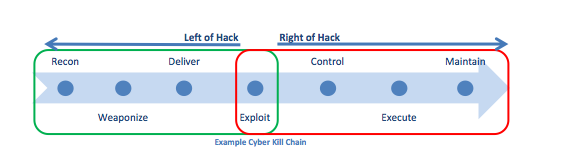
\includegraphics[scale=0.55]{./images/killChain.png}
    \caption{Cyber kill-chain \protect\cite{b1}}
\end{figure}

Como se ve en la figura~\ref{fig:kill_chain}, los primeros pasos de esta estrategia representan una 
oportunidad para detectar y mitigar las amenazas de forma proactiva antes de que 
al adversario realice un acceso no autorizado en los sistemas de la 
organización. En los pasos posteriores es donde se realiza la detección, 
respuesta y aseguramiento de los activos más importantes. Al entender al 
adversario, se puede tener una mejor oportunidad para descubrir sus intenciones 
y responder al ataque. Entender la amenaza permite la toma de mejores 
decisiones, dando prioridad a los recursos y así tener una ventaja ante el atacante. 
El resultado de defensas en base a inteligencia es una mejor opción que las 
respuestas a los ataques dado que estos ajustan sus operaciones basándose en el 
éxito o falla de sus intentos. En un modelo como el de la figura~\ref{fig:kill_chain} los intentos 
del adversario pueden ser reconocidos, logrando que los defensores tengan la 
posibilidad de ajustar sus tácticas para que al adversario le sea más 
difícil alcanzar sus objetivos.\\

Compartir información con socios y comunidades de confianza le permite a las 
organizaciones tener un conjunto de datos relevante para lograr una 
identificación precisa de la amenaza. Por medio de este intercambio, cada organización 
puede entender mejor las amenazas, no 
solo de forma abstracta sino que también con evidencias específicas que 
indiquen la presencia del atacante. Las tareas de cyber inteligencia permiten 
anticipar y mitigar las amenazas antes de que sean difíciles de encontrar y 
erradicar utilizando los métodos tradicionales de detección y respuesta. Con la 
información recolectada los analistas pueden agrupar patrones de actividades 
similares, atribuir actividades a ciertos actores, identificar e implementar 
estrategias para mitigar ataques de forma rápida y anticiparse al lanzamiento de 
ataques similares en el futuro. Para aprovechar de forma adecuada los beneficios 
de la cyber inteligencia, las organizaciones deben compartir la información 
recolectada con socios de su confianza.\\

Por medio del análisis del comportamiento de los adversarios en distintos 
objetivos y en un período de tiempo adecuado, los defensores son capaces de 
identificar un conjunto importante de indicadores, tácticas, técnicas y 
procedimientos. De esta forma se obtiene información de los objetivos y las 
estrategias lo cual permite al defensor predecir el comportamiento del atacante y 
generar defensas dinámicas. Dada la forma y complejidad con la cual evolucionan 
las amenazas, la velocidad con la cual ocurren los eventos y la basta cantidad 
de datos que se deberían intercambiar, es necesario establecer una forma 
automática para ayudar a los analistas y tomadores de decisión a llevar a cabo 
acciones defensivas.\\

Existen múltiples métodos para el intercambio de información y estos juegan un rol 
importante en los tipos, volúmenes y naturaleza de la información compartida 
con la comunidad. Algunos de estos medios de intercambio limitan el tipo de 
contenido que es compartido mientras que otros promueven ciertos tipos de 
intercambio. Los procesos para compartir información son manuales, llevan mucho 
tiempo, son repetitivos y en muchos casos requieren que las organizaciones 
reescriban o traduzcan la información a una amplia variedad de formatos. Otro 
problema que se presenta cuando se quiere intercambiar información es la 
utilización de tecnologías y/o formatos propietarios, esto provoca la necesidad 
de desarrollar scripts y módulos para permitir compartir información por fuera 
de las comunidades. Para aquellas comunidades con algún grado de automatización, 
sus modelos son generalmente bajos en prestaciones y usan soluciones 
propietarias, comerciales o adaptadas a su comunidad.\\

La mayoría de dichos 
métodos no permiten el consumo de información de amenazas de forma automática, 
esto hace que rutinariamente las organizaciones deban tomar dicha información y 
sintetizarla en sus bases de datos locales. Si bien los métodos utilizados en la 
actualidad han ayudado a mejorar las capacidades defensivas de numerosas 
organizaciones, éstas no han logrado explotar su máximo potencial.\\

La automatización requiere de información de calidad, esto 
no puede ser logrado adecuadamente con los distintos productos y sistemas de hoy en 
día. Para lograr un nivel adecuado de automatización es necesario contar con un 
estándar el cual tenga representaciones estructuradas de información, de ésta 
forma se puede lograr un mejor aprovechamiento de los datos sin saber de 
antemano quien los provee. Dicha información debe ser legible por un humano y 
parseable por una máquina. Estos requerimientos tienen varias justificaciones, 
primero que nada, un analista podría realizar un análisis que es inapropiado 
para ser automatizado o que sea focalizado en tomas de decisiones por parte de 
personas. También podría ser de interés que un analista tenga conocimiento de la 
situación actual,  de la fidelidad de las fuentes o de los métodos utilizados 
para producir la información. Por lo dicho anteriormente, es necesario la 
existencia de un estándar con una representación estructurada de la información, siendo ésta 
expresiva, flexible, extensible, automatizable y legible. Además se deben contar 
con medios para permitir el intercambio seguro y confiable de información entre 
distintas organizaciones.\\

Si bien existen varios esfuerzos para crear herramientas con las características 
presentadas, la realidad es que ninguno de ellos ha logrado su cometido. El 
objetivo de dicha herramienta debería ser:
\begin{itemize}
  \item Permitir compartir información de forma más rápida y precisa.
  \item Reducir el análisis humano y liberar a los recursos humanos para 
  realizar trabajo de análisis más valioso.
  \item Permitir que las amenazas más conocidas sean analizadas por 
  computadoras.
  \item Permitir que se comparta de forma automática un gran número de datos, 
  siendo estos datos complejos. Esto debería permitir una defensa activa.
  \item Proteger la información intercambiada.
  \item Permitir que se agregue información a las bases locales con discreción y 
  limitando el número de analistas que acceden a la información. Dicha 
  información debe tener datos de contexto.
  \item Permitir la colaboración de analistas de distintas organizaciones en los 
  incidentes.
\end{itemize}


\section{Contexto}
\label{capitulo1:contexto}
Este proyecto se desarrolla en el contexto de los temas de investigación y trabajo desarrollados en el Instituto de Computación, en particular dentro del grupo de seguridad informática (GSI) y del equipo de Respuesta a incidentes de Tilsor S.A (CSIRT Tilsor). Se interaccionará y coordinará eventualmente con otras personas y/o organizaciones que estén trabajando en temas afines.

\section{Motivación}
\label{capitulo1:motivacion}
Históricamente, se ha visto un aumento en la sofisticación, velocidad, impacto y 
cantidad de los ataques informáticos. Por ello es necesario que las estrategias 
de defensa se adapten a los nuevos actores y ataques. Para responder a esto, las 
organizaciones han tenido que recurrir al intercambio de información de amenazas 
con el fin de tener un mejor panorama de las actividades de sus adversarios 
y así ayudar a administrar sus recursos de forma de obtener el mejor resultado 
posible de sus defensas. \\

Las aproximaciones tradicionales de seguridad tienen como objetivo entender y 
registrar vulnerabilidades, debilidades y configuraciones necesarias pero 
insuficientes. Para defenderse, las organizaciones tienen estrategias basadas en 
alertas que buscan bloquear los ataques y arreglar las vulnerabilidades. Si bien dichas estrategias pueden ser efectivas contra algunas 
amenazas no logran detener ataques avanzados o proveer información sobre las 
actividades de un atacante luego de que ingresó a la red. Una estrategia más 
adecuada es basarse en \textbf{\textit{cyber kill-chain}}, en esta estrategia se busca 
descomponer las fases de un ataque con la finalidad de obtener una mejor 
comprensión del ataque y el atacante, así como mejorar las posibilidades de 
defensa.

\begin{figure}[H]
  \centering
  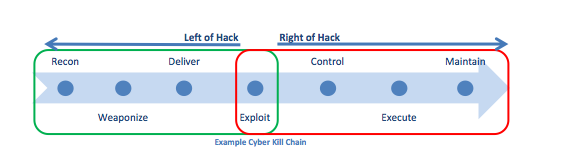
\includegraphics[scale=0.55]{./images/killChain.png}
    \caption{Cyber kill-chain \protect\cite{b1}}
      \label{fig:kill_chain}
\end{figure}

Como se ve en la figura~\ref{fig:kill_chain}, los primeros pasos de esta estrategia representan una 
oportunidad para detectar y mitigar las amenazas de forma proactiva antes de que 
al adversario realice un acceso no autorizado en los sistemas de la 
organización. En los pasos posteriores es donde se realiza la detección, 
respuesta y aseguramiento de los activos más importantes. Al entender al 
adversario, se puede tener una mejor oportunidad para descubrir sus intenciones 
y responder al ataque. Entender la amenaza permite la toma de mejores 
decisiones, dando prioridad a los recursos y así tener una ventaja ante el atacante. 
El resultado de defensas en base a inteligencia es una mejor opción que las 
respuestas a los ataques dado que estos ajustan sus operaciones basándose en el 
éxito o falla de sus intentos. En un modelo como el de la figura~\ref{fig:kill_chain} los intentos 
del adversario pueden ser reconocidos, logrando que los defensores tengan la 
posibilidad de ajustar sus tácticas para que al adversario le sea más 
difícil alcanzar sus objetivos.\\

Compartir información con socios y comunidades de confianza le permite a las 
organizaciones tener un conjunto de datos relevante para lograr una 
identificación precisa de la amenaza. Por medio de este intercambio, cada organización 
puede entender mejor las amenazas, no 
solo de forma abstracta sino que también con evidencias específicas que 
indiquen la presencia del atacante. Las tareas de cyber inteligencia permiten 
anticipar y mitigar las amenazas antes de que sean difíciles de encontrar y 
erradicar utilizando los métodos tradicionales de detección y respuesta. Con la 
información recolectada los analistas pueden agrupar patrones de actividades 
similares, atribuir actividades a ciertos actores, identificar e implementar 
estrategias para mitigar ataques de forma rápida y anticiparse al lanzamiento de 
ataques similares en el futuro. Para aprovechar de forma adecuada los beneficios 
de la cyber inteligencia, las organizaciones deben compartir la información 
recolectada con socios de su confianza.\\

Por medio del análisis del comportamiento de los adversarios en distintos 
objetivos y en un período de tiempo adecuado, los defensores son capaces de 
identificar un conjunto importante de indicadores, tácticas, técnicas y 
procedimientos. De esta forma se obtiene información de los objetivos y las 
estrategias lo cual permite al defensor predecir el comportamiento del ataque y 
generar defensas dinámicas. Dada la forma y complejidad con la cual evolucionan 
las amenazas, la velocidad con la cual ocurren los eventos y la basta cantidad 
de datos que se deberían intercambiar, es necesario establecer una forma 
automática para ayudar a los analistas y tomadores de decisión a llevar a cabo 
acciones defensivas.\\

Existen múltiples métodos para el intercambio de información y estos juegan un rol 
importante en los tipos, volúmenes y naturaleza de la información compartida 
con la comunidad. Algunos de estos medios de intercambio limitan el tipo de 
contenido que es compartido mientras que otros promueven ciertos tipos de 
intercambio. Los procesos para compartir información son manuales, llevan mucho 
tiempo, son repetitivos y en muchos casos requieren que las organizaciones 
reescriban o traduzcan la información a una amplia variedad de formatos. Otro 
problema que se presenta cuando se quiere intercambiar información es la 
utilización de tecnologías y/o formatos propietarios, esto provoca la necesidad 
de desarrollar scripts y módulos para permitir compartir información por fuera 
de las comunidades. Para aquellas comunidades con algún grado de automatización, 
sus modelos son generalmente bajos en prestaciones y usan soluciones 
propietarias, comerciales o adaptadas a su comunidad.\\

La mayoría de dichos 
métodos no permiten el consumo de información de amenazas de forma automática, 
esto hace que rutinariamente las organizaciones deban tomar dicha información y 
sintetizarla en sus bases de datos locales. Si bien los métodos utilizados en la 
actualidad han ayudado a mejorar las capacidades defensivas de numerosas 
organizaciones, éstas no han logrado explotar su máximo potencial.\\

La automatización requiere de información de calidad, esto 
no puede ser logrado adecuadamente con los distintos productos y sistemas de hoy en 
día. Para lograr un nivel adecuado de automatización es necesario contar con un 
estándar el cual tenga representaciones estructuradas de información, de ésta 
forma se puede lograr un mejor aprovechamiento de los datos sin saber de 
antemano quien los provee. Dicha información debe ser legible por un humano y 
parseable por una máquina. Estos requerimientos tienen varias justificaciones, 
primero que nada, un analista podría realizar un análisis que es inapropiado 
para ser automatizado o que sea focalizado en tomas de decisiones por parte de 
personas. También podría ser de interés que un analista tenga conocimiento de la 
situación actual,  de la fidelidad de las fuentes o de los métodos utilizados 
para producir la información. Por lo dicho anteriormente, es necesario la 
existencia de un estándar con una representación estructurada de la información, siendo ésta 
expresiva, flexible, extensible, automatizable y legible. Además se deben contar 
con medios para permitir el intercambio seguro y confiable de información entre 
distintas organizaciones.\\

\section{Objetivos}
\label{capitulo1:objetivos}
Este proyecto tiene como objetivo principal profundizar en el estudio de los mecanismos para intercambiar información entre dos entidades (en particular equipos/centros de repuesta a incidentes) de forma segura, utilizando para ésto protocolos estándares, por ejemplo haciendo implementaciones que utilicen los protocolos STIX y TAXII. Asimismo, se pretende que dicha herramienta sea aplicada al menos en algún caso de estudio.


\section{Contribución del proyecto}
\label{capitulo1:contribucion}

A partir de la investigación realizada en el desarrollo del estudio del estado del arte se pudo validar, por un lado, la necesidad que tienen las organizaciones de poder intercambiar/compartir información relativa a incidentes de seguridad, y por otro, que si bien existen diversas propuestas metodológicas y tecnológicas para construir soluciones que satisfagan esas necesidades, el enfoque adoptado por la corporación MITRE, que propone los estándares STIX y TAXII,  es el que se entiende el adecuado a tomar como referencia. \\

El resultado principal de este proyecto lo constituye el diseño e implementación de un prototipo de una herramienta para el intercambio de información sensible entre organizaciones. La misma incluye una implementación básica del protocolo TAXII que se integra al conjunto de funcionalidades provistas por el sistema RTIR, que implementa servicios de gestión de tickets, y que es una extensión de RT orientada a proveer funcionalidades específicas para la gestión de incidentes que debe realizar un equipo de respuestas a incidentes de seguridad (CSIRT). La información que la herramienta permite  intercambiar está estructurada utilizada conceptos primitivos básicos del lenguaje STIX, como lo es la noción de Cyber-observable.\\

En particular el foco principal del trabajo estuvo orientado a obtener una arquitectura de la herramienta que pudiera escalar en complejidad fácilmente, adoptando una visión de dieño que permitiera que la herramienta fuera fácilmente extensible para incorporar nuevas funcionalidades, como por ejemplo, procesos que permitan sanitizar y correlacionar la información sensible que es manipulada por la herramienta.

\section{Organización del documento}
\label{capitulo1:organizacion}
El documento se organiza de la siguiente forma.

En el Capítulo 2 se presentan conceptos generales de la gestión a incidentes y los mecanismos de intercambio de información para poner en contexto el presente trabajo. En particular se mencionan RTIR, TAXII y STIX.

En el Capítulo 3 se presentan el análisis de la investigación realizada y se definen requerimientos necesarios en una herramienta de intercambio de información.

En el Capítulo 4 se plantea el diseño que busca solucionar los requerimientos planteados en el capítulo de análisis. Se describen los componentes del sistema, las decisiones de diseño realizadas, la arquitectura del sistema y la interacción entre cada uno de los componentes utilizados.

En el Capítulo 6 se explica la implementación del sistema definido junto con las herramientas y lenguajes utilizados.

En el Capítulo 7 se describe el caso de estudio planteado.

En el Capítulo 8 se presentan las conclusiones del trabajo y posibles trabajos a futuro.

Por último se presenta la bibliografía consultada y los anexos, los cuales son referenciados a lo largo del documento.

\chapter{Estado del Arte}
\label{capitulo2}

\section{Introducción}
\label{introduccion}
Históricamente, se ha visto un aumento en la sofisticación, velocidad, impacto y 
cantidad de los ataques informáticos. Por ello es necesario que las estrategias 
de defensa se adapten a los nuevos actores y ataques. Para responder a esto, las 
organizaciones han tenido que recurrir al intercambio de información de amenazas 
con el fin de tener un mejor panorama de las actividades de sus adversarios 
y así ayudar a administrar sus recursos de forma de obtener el mejor resultado 
posible de sus defensas. \\

Las aproximaciones tradicionales de seguridad tienen como objetivo entender y 
registrar vulnerabilidades, debilidades y configuraciones necesarias pero 
insuficientes. Para defenderse, las organizaciones tienen estrategias basadas en 
alertas que buscan bloquear los ataques y arreglar las vulnerabilidades. Si bien dichas estrategias pueden ser efectivas contra algunas 
amenazas no logran detener ataques avanzados o proveer información sobre las 
actividades de un atacante luego de que ingresó a la red. Una estrategia más 
adecuada es basarse en \textbf{\textit{cyber kill-chain}}, en esta estrategia se busca 
descomponer las fases de un ataque con la finalidad de obtener una mejor 
comprensión del ataque y el atacante, así como mejorar las posibilidades de 
defensa.

\begin{figure}[H]
  \label{fig:kill_chain}
  \centering
  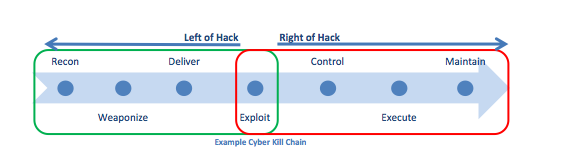
\includegraphics[scale=0.55]{./images/killChain.png}
    \caption{Cyber kill-chain \protect\cite{b1}}
\end{figure}

Como se ve en la figura~\ref{fig:kill_chain}, los primeros pasos de esta estrategia representan una 
oportunidad para detectar y mitigar las amenazas de forma proactiva antes de que 
al adversario realice un acceso no autorizado en los sistemas de la 
organización. En los pasos posteriores es donde se realiza la detección, 
respuesta y aseguramiento de los activos más importantes. Al entender al 
adversario, se puede tener una mejor oportunidad para descubrir sus intenciones 
y responder al ataque. Entender la amenaza permite la toma de mejores 
decisiones, dando prioridad a los recursos y así tener una ventaja ante el atacante. 
El resultado de defensas en base a inteligencia es una mejor opción que las 
respuestas a los ataques dado que estos ajustan sus operaciones basándose en el 
éxito o falla de sus intentos. En un modelo como el de la figura~\ref{fig:kill_chain} los intentos 
del adversario pueden ser reconocidos, logrando que los defensores tengan la 
posibilidad de ajustar sus tácticas para que al adversario le sea más 
difícil alcanzar sus objetivos.\\

Compartir información con socios y comunidades de confianza le permite a las 
organizaciones tener un conjunto de datos relevante para lograr una 
identificación precisa de la amenaza. Por medio de este intercambio, cada organización 
puede entender mejor las amenazas, no 
solo de forma abstracta sino que también con evidencias específicas que 
indiquen la presencia del atacante. Las tareas de cyber inteligencia permiten 
anticipar y mitigar las amenazas antes de que sean difíciles de encontrar y 
erradicar utilizando los métodos tradicionales de detección y respuesta. Con la 
información recolectada los analistas pueden agrupar patrones de actividades 
similares, atribuir actividades a ciertos actores, identificar e implementar 
estrategias para mitigar ataques de forma rápida y anticiparse al lanzamiento de 
ataques similares en el futuro. Para aprovechar de forma adecuada los beneficios 
de la cyber inteligencia, las organizaciones deben compartir la información 
recolectada con socios de su confianza.\\

Por medio del análisis del comportamiento de los adversarios en distintos 
objetivos y en un período de tiempo adecuado, los defensores son capaces de 
identificar un conjunto importante de indicadores, tácticas, técnicas y 
procedimientos. De esta forma se obtiene información de los objetivos y las 
estrategias lo cual permite al defensor predecir el comportamiento del atacante y 
generar defensas dinámicas. Dada la forma y complejidad con la cual evolucionan 
las amenazas, la velocidad con la cual ocurren los eventos y la basta cantidad 
de datos que se deberían intercambiar, es necesario establecer una forma 
automática para ayudar a los analistas y tomadores de decisión a llevar a cabo 
acciones defensivas.\\

Existen múltiples métodos para el intercambio de información y estos juegan un rol 
importante en los tipos, volúmenes y naturaleza de la información compartida 
con la comunidad. Algunos de estos medios de intercambio limitan el tipo de 
contenido que es compartido mientras que otros promueven ciertos tipos de 
intercambio. Los procesos para compartir información son manuales, llevan mucho 
tiempo, son repetitivos y en muchos casos requieren que las organizaciones 
reescriban o traduzcan la información a una amplia variedad de formatos. Otro 
problema que se presenta cuando se quiere intercambiar información es la 
utilización de tecnologías y/o formatos propietarios, esto provoca la necesidad 
de desarrollar scripts y módulos para permitir compartir información por fuera 
de las comunidades. Para aquellas comunidades con algún grado de automatización, 
sus modelos son generalmente bajos en prestaciones y usan soluciones 
propietarias, comerciales o adaptadas a su comunidad.\\

La mayoría de dichos 
métodos no permiten el consumo de información de amenazas de forma automática, 
esto hace que rutinariamente las organizaciones deban tomar dicha información y 
sintetizarla en sus bases de datos locales. Si bien los métodos utilizados en la 
actualidad han ayudado a mejorar las capacidades defensivas de numerosas 
organizaciones, éstas no han logrado explotar su máximo potencial.\\

La automatización requiere de información de calidad, esto 
no puede ser logrado adecuadamente con los distintos productos y sistemas de hoy en 
día. Para lograr un nivel adecuado de automatización es necesario contar con un 
estándar el cual tenga representaciones estructuradas de información, de ésta 
forma se puede lograr un mejor aprovechamiento de los datos sin saber de 
antemano quien los provee. Dicha información debe ser legible por un humano y 
parseable por una máquina. Estos requerimientos tienen varias justificaciones, 
primero que nada, un analista podría realizar un análisis que es inapropiado 
para ser automatizado o que sea focalizado en tomas de decisiones por parte de 
personas. También podría ser de interés que un analista tenga conocimiento de la 
situación actual,  de la fidelidad de las fuentes o de los métodos utilizados 
para producir la información. Por lo dicho anteriormente, es necesario la 
existencia de un estándar con una representación estructurada de la información, siendo ésta 
expresiva, flexible, extensible, automatizable y legible. Además se deben contar 
con medios para permitir el intercambio seguro y confiable de información entre 
distintas organizaciones.\\

Si bien existen varios esfuerzos para crear herramientas con las características 
presentadas, la realidad es que ninguno de ellos ha logrado su cometido. El 
objetivo de dicha herramienta debería ser:
\begin{itemize}
  \item Permitir compartir información de forma más rápida y precisa.
  \item Reducir el análisis humano y liberar a los recursos humanos para 
  realizar trabajo de análisis más valioso.
  \item Permitir que las amenazas más conocidas sean analizadas por 
  computadoras.
  \item Permitir que se comparta de forma automática un gran número de datos, 
  siendo estos datos complejos. Esto debería permitir una defensa activa.
  \item Proteger la información intercambiada.
  \item Permitir que se agregue información a las bases locales con discreción y 
  limitando el número de analistas que acceden a la información. Dicha 
  información debe tener datos de contexto.
  \item Permitir la colaboración de analistas de distintas organizaciones en los 
  incidentes.
\end{itemize}


\section{Gestión de incidentes}
\label{gestiondeincidentes}
\subsection{Herramientas}
\label{herramientas}
\subsubsection{Que es RTIR}
RTIR es un sistema de manejo de incidentes diseñado para ser utilizado por los 
equipos de seguridad de sistemas. A sido creado en conjunto con equipos de CERT 
y CSIRT para manejar el creciente número de incidentes reportados.
Presenta la ventaja de ser opensource, contener una API completa y una comunidad 
de usuarios grande y experta. Además es simple de integrar con otras 
herramientas existentes. Está implementado por medio de módulos PERL y las 
herramientas que provee RT. Se puede pensar en RTIR como una extensión de RT 
para ser utilizada por CERT's y CSIRT's.

Existen algunas alternativas a RTIR como lo son AIRT (Application for Incident Response Teams) 
cuya última versión data de Julio de 2009. AIRT es una aplicación web 
desarrollada para los equipos de respuesta a incidentes. Busca proveer facilidad 
ante los reportes de incidentes de seguridad así como un seguimiento simple de 
estos. Este sistema no cuenta con una comunidad comparable a la de RTIR así como 
con documentación tan extensa como la de RTIR.

Otra de las opciones existentes es OTRS (Open Technology Real Services), así 
como los anteriores también es open soruce. Presenta las ventajas de tener una 
comunidad más numerosa que AIRT y que el código esta siendo desarrollado continuamente. 
Así como RTIR esta desarrollado por medio de Perl y permite conectarse a varias 
bases de datos. Presenta documentación extensa para implementadores.

\section{Representación}
\label{representacion}
\subsection{Modelos de datos}
\label{modelodedatos}
%Aca se podria poner algo de openIOC

\subsubsection{IDMEF}

Intrusion Detection Message Exchange Format (IDMEF) fue especificado como un 
protocolo experimental que no especifica ningún estándar. El propósito de 
IDMEF es definir formatos de datos y procedimientos de intercambio para 
compartir información de interés con sistemas de detección de intrusos y 
sistemas de respuesta con los sistemas de administración que deben 
interactuar con estos. El RFC de IDMEF describe el modelo de datos para 
representar información tomada de los sistemas de intrusión. Se busca que dicho 
formato pueda ser utilizado por los Intrusion Detection Systems (IDSs) para 
reportar alertas sobre eventos que parezcan sospechosos.

Por medio de la firma digital de XML se busca proveer integridad, autenticidad de 
los mensajes y de los servicios. La responsabilidad para la integridad y 
autenticación de los mensajes es responsabilidad del protocolo de comunicación y 
no del formato de mensajes. La inclusión de firmas digitales en mensajes IDMEF 
debería ser realizada en casos en los que éstas deban ser archivadas para su uso 
posterior o cuando los mensajes IDMEF son intercambiados sobre protocolos poco 
seguros.

\paragraph{Modelo de datos de IDMEF}
El modelo de datos de IDMEF es una representación orientada a alertas enviadas a 
los administradores desde los sistemas de intrusión. El modelo de datos presenta 
varios problemas referentes a la representación de los datos:
\begin{itemize}
  \item Generalmente, la información de las alertas es heterogénea. Algunas 
  alertas son definidas con poca información, otras proveen información más 
  detallada. Ejemplos de alertas con poca información son aquellas que solo 
  presentan datos de origen, destino, nombre u hora, estos datos pueden set 
  extendidos por alertas detalladas en las cuales se presenta información de 
  usuarios, procesos o puertos de servicios. Es necesario que el modelo de datos 
  que represente dicha información sea flexible para adaptarse a las distintas 
  necesidades. Un modelo de datos orientado a objetos es extensible por medio de 
  agregación y sub clases, de esta forma una implementación que no entienda 
  estas extensiones podrá seguir entendiendo el subconjunto de información que 
  está definido en el modelo. Estas dos formas de extender el modelo permiten 
  que se mantenga su consistencia.
  \item Los IDSs son diferentes, algunos de estos detectan ataques analizando el 
  tráfico en la red, otros utilizando los logs de sistemas operativos o 
  aplicaciones que auditan información. Las alertas generadas para un mismo 
  ataque pero por medio de diferentes herramientas, no necesariamente contienen 
  los mismos datos. El modelo de datos define clases que soportan las 
  diferencias en las fuentes de los datos. En particular, las nociones de 
  fuente y objetivo para la alerta son representadas por una combinación de 
  nodo, procesos, servicio y clases de usuario.
  \item Dependiendo del tipo de red o sistema operativo utilizado, los 
  ataques serán observados y reportados de manera diferente lo cual lleva a que 
  el modelo de datos deba adaptarse a dichas diferencias.
  \item Los instrumentos comerciales persiguen objetivos diferentes. Por varias 
  razones, estos desean entregar más o menos información sobre ciertos tipos de 
  ataques. El modelo debe permitir la flexibilidad necesaria preservando su 
  integridad.
\end{itemize}

El diseño del modelo de datos busca proveer una representación estándar de las 
alertas de manera que la información no sea ambigua y que se describa la 
relación entre alertas simples y complejas.

El objetivo de dicho modelo es proveer una representación estándar de la 
información analizada por un sistema de intrusión cuando es detectado 
un evento inusual. Estas alertas pueden ser simples o complejas 
dependiendo de las capacidades de la herramienta que las creo.

Los nuevos objetos son introducidos para referenciar contenido adicional. Esto 
es importante debido a que la tarea de clasificar y nombrar vulnerabilidades es 
difícil y sumamente subjetiva. El modelo de datos no debe ser ambiguo, por lo 
que mientras que se permite que los análisis sean más o menos precisos 
entre ellos, no se debe permitir que estos produzcan información contradictoria  
en dos alertas que describen el mismo evento. De todas formas, siempre es 
posible insertar toda la información útil de un evento en campos de extensión 
de la alerta en lugar de en los campos a los que estos pertenecen, sin embargo, 
dichas prácticas reducen la interoperabilidad y deberían ser evitadas en lo 
posible.



\subsubsection{IODEF}

\textit{Incident Object Description Exchange Format} (IODEF) define una representación de datos que provee un framework para el 
intercambio de información entre CSIRTs, dicho tipo de información de seguridad 
es comúnmente intercambiado entre este tipo de organizaciones. IODEF provee una 
representación en XML para transportar información de incidentes entre pares en 
distintos dominios administrativos pero que tienen las responsabilidades 
operacionales de remediar o analizar y establecer advertencias en un dominio 
definido. El modelo de datos provisto por IODEF codifica la información 
referente a hosts, redes y servicios corriendo en estos sistemas; metodología 
de ataques y evidencia forense asociada; impacto de la actividad realizada y
aproximaciones a los trabajos realizados.\\

IODEF debería ser compatible con IDMEF y tener la capacidad de incluir mensajes 
IDMEF. Los actores principales en IODEF son los CSIRTs y no los IDSs como ocurre 
en IDMEF. Se puede ver a IODEF como una interfaz orientada a ser utilizada por 
personas, por ello un mensaje IODEF es parseable por una máquina y a su vez 
leíble por humanos. Los objetos IODEF tienen un tiempo de vida mayor a IDMEF, 
en éste último los mensajes son utilizados una sola vez. Los mensajes IODEF consideran 
información referente al manejo de incidentes, almacenamiento de dicha 
información o estadísticas y análisis.\\

El objetivo primordial de IODEF es mejorar las capacidades operacionales de los 
CSIRTs. La adopción por parte de la comunidad provee una habilidad mejorada para 
resolver los incidentes y transmitir información de contexto simplificando la 
colaboración e intercambio de datos.
El formato estructurado provisto por IODEF permite:
\begin{itemize}
  \item Incrementar la automatización en el procesamiento de los datos.
  \item Bajar el esfuerzo necesario para normalizar datos similares de 
  diferentes fuentes.
  \item Un formato común con el cual construir herramientas interoperables para 
  el manejo de incidentes y análisis subsecuente, específicamente cuando 
  los datos provienen de dominios distintos.
\end{itemize}

La coordinación entre CSIRTs no es un problema estrictamente técnico. La 
confianza, los procedimientos y las leyes son consideraciones que pueden impedir 
que las organizaciones intercambien información. IODEF no busca evadir dichas 
consideraciones, sin embargo, las implementaciones operacionales de IODEF deben 
considerar este contexto.

\paragraph{Modelo de datos de IODEF}\ \\

A la hora de diseñar IODEF se realizaron ciertas consideraciones de diseño:
\begin{itemize}
  \item El modelo de datos sirve como formato de transporte, lo que lleva a que 
  su representación específica no sea óptima para almacenamiento en disco, 
  ser archivado por plazos largos o procesamiento en memoria.
  \item Por medio de la implementación no se busca establecer un consenso 
  respecto a la definición de un incidente, en su lugar se trata de dar un 
  entendimiento amplio que sea lo suficientemente flexible para abarcar la 
  mayoría de las operaciones.
  \item Describir un incidente para todas las definiciones requeriría un modelo 
  de datos extremadamente complejo. Por ello, IODEF solo busca dar un marco para 
  transmitir información de incidentes comúnmente intercambiada. Se asegura un 
  mecanismo que pueda ser extendido para soportar información de la 
  organización así como técnicas para referenciar información mantenida por 
  fuera del modelo de datos.
  \item El dominio de análisis de seguridad no está totalmente estandarizado y 
  debe basarse en descripciones textuales. IODEF busca conseguir un balance 
  entre el contenido libre y el procesamiento automático de la información de 
  incidentes.
  \item IODEF es una de las representaciones que han sido estandarizadas.
   El modelo de datos de IDMEF influenció el diseño de IODEF.

\end{itemize}

El modelo de datos de IODEF no introduce problemas de seguridad. Este solo 
define una representación simple para información de incidentes. Como los datos 
codificados por IODEF pueden ser considerados sensibles por las partes que los 
intercambian se deben tomar precauciones para asegurar la confidencialidad 
durante el intercambio y el subsecuente procesamiento. El primero debe ser 
resguardado por un formato de mensaje, pero luego se deben tener consideraciones 
de seguridad en el sistema que procesa los datos, los almacena y archiva la 
documentación y la información derivada de éstos.\\

El formato de mensajes subyacente y el protocolo utilizado para intercambiar 
datos provee una garantía de confidencialidad, integridad y autenticidad. El uso 
de protocolos de seguridad estandarizados es recomendado, por ejemplo 
IODEF/RID.

\paragraph{Trabajo de MILE}\ \\

\textit{Managed Incident Lightweight Exchange} (MILE) es un grupo de trabajo del IETF que 
enfoca sus esfuerzos en dos áreas. La primera es el formato de datos y 
extensiones para representar incidentes y datos de indicadores con IODEF. La segunda área 
es el protocolo RID.\\

Respecto a IODEF se busca revisar el RFC para incorporar mejoras y extensiones 
basándose en la experiencia que ha sido obtenida de su utilización. Se busca poder extender IODEF para 
soportar extensiones específicas necesarias por la industria y permitir utilizar 
contenido específico. Además MILE busca proveer guías en la implementación y uso 
de IODEF para ayudar a los implementadores en el desarrollo de sistemas.\\

Respecto a RID se busca definir una aproximación orientada a los recursos que 
permita a los CSIRTs ser más dinámicos y ágiles a la hora de colaborar. También 
se busca proveer guías en la implementación y uso de RID. RID podría requerir 
modificaciones para agregar información de políticas u otros cambios. Con el 
incremento en la cantidad de implementaciones RID, podría ser necesaria una 
revisión de su RFC.



%\input{./secciones/OPENIOC}
\subsubsection{STIX}

Structured Threat Information eXpression (STIX) es un lenguaje para la especificación, captura, representación y 
comunicación de información de seguridad. Lo realiza de manera 
estructurada para soporteortar un mejor manejo de la información así como para 
permitir procesos automatizados.\\

Se busca que la información sea representada de forma estructurada, a su vez 
esta debe ser expresiva, flexible, extensible, automatizable y legible. Esto se 
presenta como un desafío ya que la información intercambiada debe ser 
estructurada para que pueda ser parseada por una máquina pero no se debe perder 
la posibilidad de que un analista la pueda leer y entender. Que sea entendible 
por una persona es necesario para que no se pierda el juicio y control que esta 
pueda tener.\\

Al convertirse STIX en un estándar para la comunidad se obtendrá información de 
mejor calidad la que será mejor aprovechada y de la cual no se sabrá la fuente 
de los datos de antemano.

\paragraph{Aproximaciones de la actualidad}\ \\

La información que se intercambia y utiliza actualmente es atómica, inconsistente 
y muy limitada en sofisticación y expresividad. Además, el uso de estructuras 
estandarizadas se enfoca en una porción del problema y la integración no se 
realiza de forma adecuada entre si o carece de la flexibilidad para hacerlo. 
Generalmente, las actividades de intercambio de indicadores son entre humanos, 
siendo los indicadores desestructurados o semi-estructurados e intercambiados 
por medio de portales web o encriptados y enviados vía email. Recientemente se 
ha visto el surgimiento de transferencias entre máquinas, éstas intercambian 
conjuntos de indicadores simples de modelos de ataques bien conocidos.\\

A diferencia de IODEF, STIX provee una lista de elementos para construir 
indicadores de compromiso y se integra con CAPEC, MAEC o CVE. Además posee 
soporte para tácticas, técnicas y procedimientos del adversario y tareas 
realizadas por la organización. IODEF fue pensado para compartir información de 
incidentes y no indicadores de compromiso. STIX permite el intercambio de 
indicadores referentes a amenazas así como información del contexto en el que 
éstas se dan. Juntos, permiten tener un conocimiento más rico de las 
intenciones, capacidades, motivaciones y actividades de un adversario y de esta 
forma defenderse de él.\\

STIX busca extender los indicadores para permitir el manejo e intercambio de 
estos de forma más expresiva y con un espectro más amplio de información.\\

Actualmente, el intercambio y manejo de información automática es visto 
típicamente en líneas de productos, servicios ofrecidos o soluciones específicas 
de una comunidad. STIX busca permitir el intercambio de información de forma 
comprensiva, rica, de alta fidelidad entre organizaciones, comunidades, 
productos y servicios ofrecidos.\\

STIX provee una arquitectura unificada con un conjunto amplio de información 
para permitir una solución práctica que permita la implementación de distintos 
casos de uso. El conjunto de información incluye:
\begin{itemize}
  \item Cyber Observables
  \item Indicadores
  \item Incidentes
  \item Tácticas, técnicas y procedimientos de los adversarios
  \item Objetivos de exploits
  \item Cursos de acción
  \item Campañas de ataques
  \item Actores de ataques
\end{itemize}


\paragraph{Casos de uso}\ \\

El lenguaje STIX ha sido desarrollado para soportar varios casos de uso involucrados en el 
manejo de amenazas de seguridad. A continuación se dan descripciones de esos 
casos de uso.
\begin{itemize}
  \item \underline{Análisis de Cyber Amenazas}: Un analista de seguridad estudia información 
  estructurada y no estructurada referente a actividades de una amenaza 
  procedentes de varias fuentes. El analista busca entender la naturaleza de las 
  amenazas más relevantes, identificarlas, y representarlas para poder expresar 
  y actualizar el conocimiento relevante de la amenaza. La información de la 
  amenaza incluye acciones realizadas, comportamientos, capacidades, quienes lo 
  realizaron, etc. De este conocimiento y representación el analista puede 
  especificar patrones de la amenaza, sugerir acciones a ser realizadas para 
  responder a sus actividades y/o compartir información con socios de su 
  confianza.
  \item \underline{Especificar patrones de amenazas}: Un analista especifica patrones para 
  representar las características de amenazas junto con su contexto y metadatos 
  para interpretar, manejar y aplicar el patrón y sus resultados. Esto puede ser 
  realizado manualmente o con la asistencia de una herramienta automática.
  \item \underline{Manejo de las actividades de respuesta}: Los encargados de tomar decisiones y el personal de operaciones trabajan 
  en conjunto para prevenir o detectar actividades que presenten una amenaza y 
  responder a los incidentes detectados que sean realizados por dichas amenazas. 
  Las acciones preventivas pueden mitigar vulnerabilidades, debilidades o malas 
  configuraciones que sean objetivos de exploits. Luego de la detección e 
  investigación de incidentes específicos, acciones reactivas pueden ser 
  realizadas. Se pueden desprender tres sub-casos de uso de lo anterior.
  \begin{itemize}
    \item \underline{Prevención de amenazas}: Quienes deben tomar las decisiones evalúan 
    acciones preventivas para las amenazas relevantes que sean identificadas. Además deben crear acciones para mitigar dichas amenazas. El personal de 
    operaciones implementa las acciones seleccionadas por los tomadores de 
    decisión. Dichas medidas preventivas son obtenidas por medio de la 
    interpretación de los indicadores.
    \item \underline{Detección de amenazas}: El personal de operaciones aplica mecanismos 
    (automáticos y manuales) para monitorear y asistir las operaciones con la 
    finalidad de detectar la ocurrencia de amenazas específicas basándose en la 
    evidencia histórica, análisis del contexto actual e interpretación de los 
    indicadores que se presentan. Esta detección se realiza generalmente por 
    medio de patrones de indicadores.
    \item \underline{Respuesta a incidentes}: El personal de operaciones responde a amenazas 
    detectadas, investiga que ha ocurrido o está ocurriendo, trata de 
    identificar y representar la naturaleza de las amenazas y lleva a cabo 
    acciones para mitigar sus efectos, también puede aplicar acciones 
    preventivas. Una vez que los efectos son entendidos, el personal de 
    operaciones puede implementar acciones acordes para prevenir o llevar a cabo 
    tareas correctivas.
  \end{itemize} 
  \item \underline{Intercambio de información}: Los encargados de tomar las decisiones 
  establecen políticas respecto a que tipo de información será compartida, 
  además toma decisiones respecto a con quienes se comparte y como debería ser 
  manejada basándose en frameworks de confianza de forma de mantener niveles 
  adecuados de consistencia, contexto y control. Esta política es luego 
  implementada para compartir los indicadores de amenazas apropiados y otra 
  información de amenazas.
\end{itemize}

\paragraph{Principios de desarrollo de STIX}\ \\
En el enfoque dado a STIX se ha buscado implementar un conjunto de principios 
para su desarrollo con el consenso de la comunidad. Esos principios son los siguientes:
\begin{itemize}
  \item \underline{Expresividad}: Con el fin de soportar la diversidad de casos de uso relevantes, STIX apunta a 
proveer una cobertura expresiva en todos sus casos de uso específicos en lugar 
de dirigirse específicamente a alguno de ellos.
  \item \underline{Integración en lugar de duplicación}: Cuando STIX abarca conceptos de información estructurada para los cuales ya 
existen representaciones estandarizadas con el consenso adecuado y que se 
encuentran disponibles, se busca integrar estas representaciones a la 
arquitectura STIX en lugar de duplicar esta información innecesariamente.
\item \underline{Flexibilidad}: Con el fin de soportar un amplio rango de casos e información variable con 
varios niveles de fidelidad, se ha diseñado a STIX para ofrecer tanta flexibilidad 
como sea posible. STIX se adhiere a una política de permitir a los usuarios 
utilizar cualquier porción de representaciones estándar que sean relevantes para 
un contexto dado y evita elementos obligatorios siempre que sea posible.
\item \underline{Extensibilidad}: Con la finalidad de soportar un amplio rango de casos de uso con un potencial 
diferente de representación y para facilitar el perfeccionamiento 
impulsado por la comunidad, se ha diseñado STIX para construir mecanismos de 
extensión para usos específicos, para usos localizados, para refinamientos del 
usuario y evolución y para facilidad de refinamiento y evolución centralizada.
\item \underline{Automatización}: El diseño realizado en STIX busca maximizar la estructura y la consistencia para 
soportar métodos de procesamiento automático por máquinas.
\item \underline{Lectura}: El diseño de STIX busca estructuras del contenido para que no sea únicamente 
consumible o procesable por máquinas sino que también sea leíble por humanos. 
Esto es necesario para claridad y comprensibilidad durante las primeras etapas 
de desarrollo y adopción.
\item \underline{Implementación}: La implementación inicial de STIX utiliza XML como un mecanismo portátil, 
estructurado y que se puede encontrar en cualquier parte para la discusión, 
colaboración y refinamiento entre las comunidades involucradas. Está pensado 
para el desarrollo en colaboración de un lenguaje estructurado sobre información de 
amenazas entre expertos de la comunidad. Se ha pensado que el uso del lenguaje 
sea estimulado y soportado por medio del desarrollo de varias herramientas como 
APIs. Solo por medio de niveles adecuados de colaboración entre miembros de la 
comunidad y con la utilización de datos reales se puede llegar a que la solución 
evolucione.
\end{itemize}









%  \begin{center}
%  \begin{longtable}{|1|1|}
%  \caption{}
%  
%  \hline \multicolumn{1}{|c|}{\textbf{STIX}} & \multicolumn{1}{c|}{IODEF} \\ \hline 
%  \endfirsthead
%  
%  \multicolumn{2}{c}%
%  {{\bfseries \tablename\ \thetable{} -- sigue en la página siguiente}} \\
%  \hline \multicolumn{1}{|c|}{STIX} &
%  \multicolumn{1}{c|}{IODEF} \\ \hline 
%  \endhead
%  
%  \hline \multicolumn{2}{|r|}{{Sigue en la página siguiente}} \\ \hline
%  \endfoot
%  
%  \hline \hline
%  \endlastfoot
%  \pbox{7cm}{Se representan observables que son propiedades o eventos que se dan durante las operaciones de redes o computadores. Se refiere a información sobre un archivo, una key en la registry, un servicio iniciado, etc. Para su representación se utiliza CyBox. Se da información de eventos en el host y la red por medio de Observables. Se puede considerar información como nombres, hashes, tamaños de archivos. Keys que se cambian en la registry, servicios que se ejecutan o request realizadas a un host (ie: request http)} & \pbox{7cm}{Descripción de eventos particulares del incidente que se dan en un host o red. También se puede tener información de Log de los eventos o acciones significativas realizadas por los involucrados.} \\
%  \pbox{7cm}{Se representa información de indicadores que afectan a la organización así como nuevos datos conocidos durante la respuesta al incidente. Se dan datos sobre lo que busco realizar un atacante, fuente de la información del incidente y tareas realizadas por los analistas.} & \pbox{7cm}{Se da una descripción textual del incidentes. Se da información de contacto de las partes que participaron del incidente.  Se da información de la razón por la cual se envía el documento y de cuales son las posibilidades que tiene el receptor para divulgar información.} \\
%   & \pbox{7cm}{Se permite la extensión del modelo para representar datos que no están en éste.} \\
%  \pbox{7cm}{Se da información sobre socios involucrados.} & \pbox{7cm}{Información de contacto para personas u organizaciones involucradas en el incidente.} \\
%  \pbox{7cm}{La clase Incidents da representaciones de los tiempos de detección reporte, etc del incidentes.} & \pbox{7cm}{La clases Time dan información sobre el comienzo, fin, detección del incidente.} \\
%  \pbox{7cm}{Se da una representación del modus operandi del adversario. Esto se realiza por medio de TTP, en estas se busca representar comportamientos específicos que muestra el adversario, recursos que éste tiene como herramientas e infraestructura, información de las victimas, objetivos de exploits, fuentes de la información de los TTP. Se utilizan otros estándares como CVE, CAPEC o MAEC para la representación de los ataques o del malware.} & \pbox{7cm}{Una representación libre de la metodología utilizada por el adversario. Se representan las técnicas utilizadas por el atacante.} \\
%  \pbox{7cm}{Por medio de la clase incidents se da información de bienes afectados y de la naturaleza del incidente.} & \pbox{7cm}{Repercusiones técnicas y no técnicas del incidente, ie: impacto monetario, de tiempo, etc.} \\
%  \pbox{7cm}{Las campaigns dan referencia a actividades similares que fueron realizadas.} & \pbox{7cm}{Referencia a actividades similares.} \\
%  \pbox{7cm}{Representación de campañas, esto son adversarios con una intención. Las campañas consisten de las intenciones del adversario, sus TTP utilizadas en la campaña, los incidentes realizados en la campaña, indicadores asociados a la campaña.} &  \\
%  \pbox{7cm}{Representaciones de adversarios que tienen ciertas intenciones y han sido observados históricamente. Los adversarios tienen las siguientes características: una representación de identidad, se sospecha de una motivación, una intención de conseguir algo, tienen un historial de TTP, ciertas campaigns son asociadas con un adversario, etc.} &  \\
%  \pbox{7cm}{Se representan objetivos de exploits, estos se pueden ver como vulnerabilidades en software, sistemas, configuraciones de red que son objetivos para ser explotados por las TTP de un adversario. Se utilizan CVE, OSVBD (entre otras) para la identificación de vulnerabilidades publicas.} & \pbox{7cm}{Se da una clasificación de vulnerabilidades conocidas.} \\
%  \pbox{7cm}{Se representan medidas que deberían ser realizadas para prevenir o corregir para evitar ser objetivo de exploits.} & \pbox{7cm}{Se dan acciones que debería realizar el receptor.} \\
%  \pbox{7cm}{Se representan etiquetas para la información que indican restricciones o datos potencialmente sensibles.} &  \\ 
%  \end{longtable}
%  \end{center}


\begin{center}
\begin{longtable}{|c|c|c|c|}
\caption{Comparativa de STIX e IODEF}\\
\hline
\textbf{STIX} & \textbf{IODEF}  \\
\hline
\endfirsthead
\multicolumn{4}{c}%
{\tablename\ \thetable\ -- \textit{Continuación de la página anterior}} \\
\hline
\textbf{STIX} & \textbf{IODEF}  \\
\hline
\endhead
\hline \multicolumn{4}{r}{\textit{Continua en la página siguiente}} \\
\endfoot
\hline
\endlastfoot
  \pbox{7cm}{Se representan observables que son propiedades o eventos que se dan durante las operaciones de redes o computadores. Se refiere a información sobre un archivo, una key en la registry, un servicio iniciado, etc. Para su representación se utiliza CyBox. Se da información de eventos en el host y la red por medio de Observables. Se puede considerar información como nombres, hashes, tamaños de archivos. Keys que se cambian en la registry, servicios que se ejecutan o request realizadas a un host (ie: request http)} & \pbox{7cm}{Descripción de eventos particulares del incidente que se dan en un host o red. También se puede tener información de Log de los eventos o acciones significativas realizadas por los involucrados.} \\  
  \hline
  \pbox{7cm}{Se representa información de indicadores que afectan a la organización así como nuevos datos conocidos durante la respuesta al incidente. Se dan datos sobre lo que busco realizar un atacante, fuente de la información del incidente y tareas realizadas por los analistas.} & \pbox{7cm}{Se da una descripción textual del incidentes. Se da información de contacto de las partes que participaron del incidente.  Se da información de la razón por la cual se envía el documento y de cuales son las posibilidades que tiene el receptor para divulgar información.} \\ 
  \hline
   & \pbox{7cm}{Se permite la extensión del modelo para representar datos que no están en éste.} \\ 
   \hline
  \pbox{7cm}{Se da información sobre socios involucrados.} & \pbox{7cm}{Información de contacto para personas u organizaciones involucradas en el incidente.} \\ 
  \hline
  \pbox{7cm}{La clase Incidents da representaciones de los tiempos de detección reporte, etc del incidentes.} & \pbox{7cm}{La clases Time dan información sobre el comienzo, fin, detección del incidente.} \\ 
  \hline
  \pbox{7cm}{Se da una representación del modus operandi del adversario. Esto se realiza por medio de TTP, en estas se busca representar comportamientos específicos que muestra el adversario, recursos que éste tiene como herramientas e infraestructura, información de las victimas, objetivos de exploits, fuentes de la información de los TTP. Se utilizan otros estándares como CVE, CAPEC o MAEC para la representación de los ataques o del malware.} & \pbox{7cm}{Una representación libre de la metodología utilizada por el adversario. Se representan las técnicas utilizadas por el atacante.} \\ 
  \hline
  \pbox{7cm}{Por medio de la clase incidents se da información de bienes afectados y de la naturaleza del incidente.} & \pbox{7cm}{Repercusiones técnicas y no técnicas del incidente, ie: impacto monetario, de tiempo, etc.} \\ 
  \hline
  \pbox{7cm}{Las campaigns dan referencia a actividades similares que fueron realizadas.} & \pbox{7cm}{Referencia a actividades similares.} \\ 
  \hline
  \pbox{7cm}{Representación de campañas, esto son adversarios con una intención. Las campañas consisten de las intenciones del adversario, sus TTP utilizadas en la campaña, los incidentes realizados en la campaña, indicadores asociados a la campaña.} &  \\ 
  \hline
  \pbox{7cm}{Representaciones de adversarios que tienen ciertas intenciones y han sido observados históricamente. Los adversarios tienen las siguientes características: una representación de identidad, se sospecha de una motivación, una intención de conseguir algo, tienen un historial de TTP, ciertas campaigns son asociadas con un adversario, etc.} &  \\ 
  \hline
  \pbox{7cm}{Se representan objetivos de exploits, estos se pueden ver como vulnerabilidades en software, sistemas, configuraciones de red que son objetivos para ser explotados por las TTP de un adversario. Se utilizan CVE, OSVBD (entre otras) para la identificación de vulnerabilidades publicas.} & \pbox{7cm}{Se da una clasificación de vulnerabilidades conocidas.} \\ 
  \hline
  \pbox{7cm}{Se representan medidas que deberían ser realizadas para prevenir o corregir para evitar ser objetivo de exploits.} & \pbox{7cm}{Se dan acciones que debería realizar el receptor.} \\ 
  \hline
  \pbox{7cm}{Se representan etiquetas para la información que indican restricciones o datos potencialmente sensibles.} &  \\  
  \hline
\end{longtable}
\end{center}


\subsection{Estándares}
\label{estandares}
\section{Intercambio}
\label{intercambio}
\subsection{Protocolos}
\label{protocolos}
%En este punto hay que poner algo de cybex, no es un protocolo sino un framework
\subsubsection{RID}

\textit{Real-Time Inter-Network} (RID) es un método de comunicación entre redes para 
facilitar el intercambio de datos de incidentes. A su vez, busca integrar 
mecanismos existentes de detección, seguimiento, identificación de fuentes y 
mitigación que aporta una solución al manejo de incidentes. Combinar estas 
capacidades en un sistema de comunicación permite incrementar el nivel de 
seguridad en la red. Las políticas para manejar incidentes son recomendadas y 
pueden ser acordadas por un consorcio utilizando recomendaciones y 
consideraciones de seguridad.\\

RID ha sido ampliamente utilizando en comunidades de investigación, pero no ha 
sido muy adoptado por otros sectores. Fue desarrollado como un mecanismo de 
comunicación para facilitar la transferencia de información entre distintos 
proveedores de servicios de Internet para trazar precisa y eficientemente el 
flujo de paquetes nocivos a lo largo de la red.\\

Los datos en RID son representados como documentos XML utilizando IODEF. De esta 
forma se simplifica la integración con otros aspectos del manejo de incidentes.\\ 

Se deben utilizar 
conexiones autenticadas y encriptadas entre sistemas RID para proveer 
confidencialidad, integridad, autenticidad y privacidad de los datos. \\

RID requiere una 
especificación de un protocolo de transporte para asegurar la interoperabilidad 
entre las organizaciones socias. El RFC6046 mencionado anteriormente, especifica 
el transporte de mensajes RID sobre HTTPS/TLS. 












 
\subsection{TAXII}

El objetivo que plantea \textit{Trusted Automated eXchange of Indicator Information} (TAXII) es extender la capacidad de compartir indicadores, 
siendo dichos intercambios robustos, seguros y de gran volumen de datos. A su 
vez, los datos intercambiados deberían ser mas expresivos que en la actualidad.\\

Con TAXII no se busca crear una comunidad para compartir, sino que se le da a 
las organizaciones una herramienta que facilite el intercambio entre ellas. 
TAXII mejora las deficiencias existentes dando especificaciones abiertas y 
comunes para transportar los mensajes con información. También se provee un 
conjunto de capacidades como encriptación, autenticación, direccionamiento, 
alertas y pedidos entre sistemas.\\

TAXII es un conjunto de especificaciones técnicas y de documentación para 
permitir el intercambio de información procesable entre organizaciones. Para 
realizar dichos intercambios, se definen protocolos y formatos de datos que 
permiten intercambiar información de forma segura. Ha sido diseñado para permitir la
interoperabilidad de diferentes soluciones en lugar de ligarse a una tecnología o producto en particular.
Además, se busca incentivar a los proveedores de tecnología a incorporar soporte para las especificaciones
de TAXII en sus productos. La información intercambiada 
ayuda a detectar, prevenir y mitigar amenazas informáticas en tiempo real. Es 
importante recalcar que no se buscan definir acuerdos para el intercambio de 
información o gobierno. En su lugar, permite a las organizaciones mejorar el 
contexto en el que se encuentran respecto a las nuevas amenazas y además 
compartir la información que ellos elijan con las organizaciones que deseen de 
forma simple y rápida aprovechando las relaciones y sistemas existentes.\\

Al igual que en STIX, en TAXII se buscó consenso y participación de la comunidad. 
TAXII permite el intercambio de información sobre amenazas de forma eficiente y 
comprensiva por medio de \emph{automatización} y \emph{articulación} de un 
modelo detallado de información. Para lograr esto, se utiliza una representación 
estándar de información de amenazas y un framework para soportar el intercambio 
de datos. El modelo permite el envío y recepción de un conjunto amplio de 
información de seguridad para soportar las necesidades referentes al intercambio 
de información. Se le da la libertad a los proveedores de determinar como sus 
productos producen, consumen o toman ventaja de los flujos de información 
especificados por TAXII.\\

 
\begin{figure}[ht!]
  \centering
    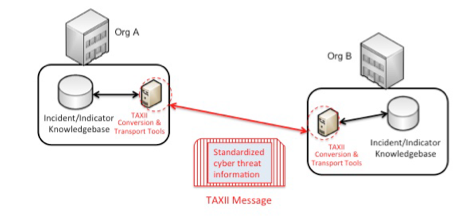
\includegraphics[scale=0.80]{./images/TAXIIArchitecture1.png}
    \caption{Arquitectura de TAXII \protect\cite{b1}}
    \label{fig.diagramabloques}
\end{figure}

TAXII utiliza protocolos y especificaciones existentes siempre que 
es posible, de esta forma se integra con mecanismos de intercambio de 
información para reducir los costos de implementación y permitir la adopción 
rápida por parte de organizaciones ya establecidas y que se encuentran 
intercambiando información.\\

Las motivaciones para tener una mejor solución que permita intercambiar 
información lleva a que en el diseño de TAXII se hayan planteado los siguientes 
objetivos:
 \begin{itemize}
   \item Permitir el intercambio seguro y rápido de información referente a 
   amenazas entre comunidades de defensores de seguridad.
   \item Lograr un estándar para permitir compartir indicadores entre organizaciones.
   \item Extender el intercambio de indicadores para permitir intercambios 
   seguros, robustos y de gran volumen que tengan una expresividad mayor a la 
   actual.
   \item Soportar un amplio número de casos de uso y prácticas comunes a las 
   comunidades.
   \item Tomar los estándares existentes que sean adecuados.
   \item Llegar a una adopción por parte de organizaciones internacionales de 
   estándares.
 \end{itemize}

Para automatizar el intercambio de información, es necesario especificar como 
ésta es compartida. Para lograr esto, TAXII define especificaciones técnicas y 
documentación de soporte. En particular, las especificaciones de TAXII definen 
un conjunto de capacidades necesarias para el transporte exitoso de mensajes. 
Los mensajes TAXII llevan datos de amenazas informáticas representados por medio de STIX. El conjunto completo de los mensajes incluyen mensajes con datos y 
de control.\\

\subsubsection{TAXII Toolkit}\ \\

Es provisto para soportar la adopción de TAXII y asistir en el desarrollo de 
capacidades compatibles. El \textit{toolkit} provee una colección de implementaciones de 
referencia, un conjunto de herramientas y una colección de librerías e 
interfaces.\\

TAXII está definido por múltiples especificaciones relacionadas. Esta sección 
describe las especificaciones definidas en TAXII.

\begin{itemize}
  \item \underline{Especificación de servicios}: Provee los requerimientos por los cuales se 
  definen los servicios e intercambios de TAXII. No provee detalles respecto al 
  formato de los datos o como los mensajes TAXII son transportados por la red. 
  Dichos detalles y requerimientos pueden ser encontrados en la especificación 
  de los protocolos de enlace y en la especificación de mensajes de enlace.
 \item \underline{Especificación de protocolos de enlace}: Define los requerimientos para 
 transportar mensajes TAXII por la red. Puede haber varias especificaciones 
 creadas para TAXII. Cada especificación define requerimientos para el 
 transporte de mensajes TAXII utilizando protocolos de red y se proveen 
 requerimientos respecto a como los servicios TAXII son soportados por los 
 protocolos de red.
 \item \underline{Especificación de mensajes de enlace}: Se definen requerimientos para 
 representar mensajes TAXII en un formato particular. Puede haber múltiples 
 especificaciones para dichos mensajes. Se provee información detallada sobre 
 como las especificaciones definidas en la especificación de servicios son 
 expresadas en los mensajes.
\end{itemize}

Para dar flexibilidad en el proceso evolutivo de TAXII, se han separado las 
especificaciones de servicios, de los protocolos de enlace y de los mensajes de 
enlace.
Debido a que las organizaciones generalmente tienen restricciones 
respecto a los protocolos que soportan, TAXII busca no ligarse a un único 
protocolo que excluya a una parte de la comunidad. Cuando se ve que la comunidad 
expresa interés en un nuevo protocolo o tipo de mensaje, TAXII puede dar soporte 
para ellos sin cambiar los componentes centrales.\\

Dos grupos que usen el mismo protocolo de red y formato de mensajes serán 
capaces de intercambios de información estructurada de forma automática. Las 
políticas de intercambio de los participantes pueden limitar estos intercambios 
si es necesario, pero el uso de servicios compatibles con TAXII asegura que se 
puede intercambiar cualquier información con los mecanismos definidos por TAXII. 
Los grupos que usen diferentes protocolos o formatos de mensajes no serán 
capaces de comunicarse directamente, pero como están utilizando mensajes y 
servicios en el núcleo de las comunicaciones de sus comunidades significa que es 
posible establecer caminos para que ocurra la interacción.

\subsubsection{Especificación de Servicios}\ \\

Esta especificación provee normativas respecto a los servicios, mensajes e 
intercambios de mensajes en TAXII. No provee detalles respecto a como los 
mensajes son transportados, dejando eso a la especificación de los protocolos de 
enlace. Se da información respecto a los datos presentes en los mensajes TAXII y 
no a como los mensajes son expresados.\\

Las unidades funcionales de TAXII representan conjuntos discretos de actividades 
requeridas para soportar TAXII. Una unidad funcional representa algún componente 
con un rol bien definido en TAXII.

\begin{itemize}
  \item \underline{TAXII Transfer Agent} (TTA): Es una unidad funcional conectada a la red 
  que envía o recibe mensajes TAXII. Una TTA interactúa con otras TTAs por medio 
  de la red y maneja los requerimientos de una o más de las especificaciones de 
  los protocolos de enlace. Una TTA provee un mensaje TAXII a un \textit{TAXII Message 
  Handler} permitiendo que éste último sea independiente del protocolo de red 
  utilizado. De la misma forma, el TTA puede ser independiente del contenido de 
  los mensajes TAXII, dejando el manejo de la información al \textit{TAXII Message 
  Handler}.
  \item \underline{TAXII Messsage Handler} (TMH): Es una unidad funcional que produce y 
  consume mensajes TAXII. EL TMH es responsable de parsear y construir mensajes 
  con el formato especificado en uno o más TAXII \textit{Message Binding Specifications}. 
  Un TMH interactúa con un TTA, el cual maneja los detalles necesarios para 
  transmitir mensajes por la red. El Backend TAXII interactúa con el TMH para 
  convertir su contenido en mensajes TAXII y llevar a cabo actividades basadas 
  en los mensajes TAXII que son recibidos por el TMH.
  \item \underline{Backend TAXII}: Cubre todas las unidades funcionales distintas al TTA y 
  al TMH. Las especificaciones de TAXII no proveen requerimientos sobre como son 
  implementadas las capacidades en un backend más allá de como debe interactuar 
  con el TMH. Las organizaciones o implementadores pueden decidir que 
  capacidades implementar según los servicios TAXII que deseen soportar o según 
  como quieran dar ese soporte.
  \item \underline{Arquitectura TAXII}: Cubre los aspectos de las unidades funcionales de la 
  infraestructura de productor o consumidor que provee o utiliza servicios 
  TAXII. Una arquitectura TAXII incluye una TTA, un TMH y un backend TAXII.
  \end{itemize}

Lo expresado anteriormente se puede ver en la figura \ref{fig.unidades_funcionales}.

\begin{figure}[ht!]
  \centering
    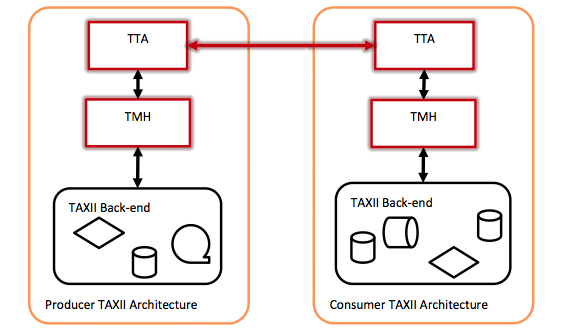
\includegraphics[width=150mm]{./images/TAXIIArchitecture.png}
    \caption{Unidades funcionales de TAXII \protect\cite{b1}}
    \label{fig.unidades_funcionales}
\end{figure}

\newpage
\subsubsection{Capacidades}\ \\

TAXII provee capacidades específicas para aquellos que desean compartir 
información de amenazas cibernéticas. Las capacidades TAXII son el nivel más 
alto en el cual se pueden expresar las acciones de TAXII. Hay tres capacidades 
que soporta la actual versión de TAXII, estas son: \textit{push messaging}, \textit{pull 
messaging} y \textit{discovery}.\\

En \textit{\textbf{push messaging}} la información puede ser enviada de un productor a un 
consumidor. Esto puede reflejar una relación pre-existente entre el productor y 
el consumidor en la que el consumidor ha pedido que se le envíen datos desde el 
productor. También puede usarse en caso de que el consumidor desee aceptar 
contribuciones de cualquier productor, y estos le envíen datos en cualquier 
momento.\\

\textit{\textbf{Pull messaging}} permite a un consumidor requerir información de un productor. 
Esto no solo le permite al consumidor el control sobre el momento en el que 
recibe los datos sino que también le permite hacerlo sin tener que aceptar 
conexiones entrantes. Así como en \textit{push messaging}, el productor y consumidor 
pueden tener acuerdos pre-existentes para que el consumidor tenga acceso a los 
datos del productor. De forma alternativa, un productor puede hacer su 
información pública de forma que cualquier consumidor pueda obtenerla. La 
versión actual de \textit{pull messaging} limita a los consumidores a hacer pedidos por 
medio de las organizaciones productoras de los datos en lugar de por los datos 
en si. Toda la información provista por un productor debe estar organizada en 
grupos llamados "TAXII Data Feeds". Cada elemento en un TAXII data feed es 
etiquetado utilizando \textit{timestamps}. El productor tiene total dominio sobre como el 
contenido se mapea en TAXII data feeds y en el significado de los \textit{timestamps}. La 
capacidad de \textit{pull messaging} está atada a entender el contenido del productor.\\

Para facilitar las comunicaciones automatizadas, TAXII soporta capacidades para 
descubrir los servicios específicos que ofrece un servidor o grupo de 
servidores, así como los protocolos o mensajes que este servidor ofrece. Esto no 
quita la necesidad de que personas estén involucradas para establecer acuerdos de 
cooperación lo cual esta por fuera del objetivo de TAXII. Sin embargo, permite 
el intercambio de información respecto a las capacidades que un productor 
soporta y cuales son los mecanismos que utiliza para hacerlo.

\subsubsection{Servicios TAXII}\ \\

Los servicios TAXII representan un conjunto de mecanismos necesarios para 
soportar capacidades TAXII. Una implementación TAXII pudiera implementar alguno, 
todos o incluso ninguno de los servicios definidos.
TAXII define los siguientes servicios:
\begin{itemize}
  \item \underline{Discovery Service}: Es utilizado para recibir y responder a 
  mensajes que requieren información sobre los servicios ofrecidos.
  \item \underline{Feed Managment Service}: Es utilizado para recibir o responder a mensajes 
  utilizados para el manejo de subscripciones a TAXII Data Feed.
  \item \underline{Inbox Service}: Es utilizado para recibir información de amenazas 
  cibernéticas por medio de intercambios iniciados por el productor en intervalos 
  dictados por este.
  \item \underline{Poll Service}: Es utilizado para recibir y responder a mensajes de pedido 
  a el TAXII Data Feed iniciados por el consumidor.
\end{itemize}

A continuación se describen los distintos servicios.

\paragraph{Discovery Service}\ \\

Es un mecanismo para comunicar información referente al uso de servicios TAXII y 
a su disponibilidad. Para un pedido al servicio, se retorna una lista de los 
servicios TAXII y como estos pueden ser invocados. Un solo servicio de 
descubrimiento puede reportar servicios TAXII en diferentes equipos finales o 
incluso en múltiples organizaciones, los propietarios del servicio pueden 
definir su alcance a gusto. Un servicio de descubrimiento puede utilizar 
varios factores para determinar cuales servicios revelar ante una petición, 
incluyendo, pero no limitado a la entidad del cliente TAXII.
El servicio de descubrimiento debe soportar "Discovery Message Exchange".

\paragraph{Feed Managment Service}\ \\

Es el mecanismo con el cual un consumidor pide información referente a TAXII 
Data Feeds, pidiendo subscripciones a estos, o modificando las existentes. Este 
servicio facilita el intercambio de mensajes para manejar las subscripciones. 
No se entrega contenido de los TAXII Data Feed, en su lugar se envía 
contenido del TAXII Data Feed al servicio de Inbox de un consumidor en intercambios 
iniciados por un productor o en respuesta directa a un pedido del consumidor al 
servicio de poll.
Dicho servicio debe implementar soporte para \textit{subscription managment exchange} y podría implementar soporte de \textit{feed information exchange}.

\paragraph{Inbox service}\ \\
Este servicio es el mecanismo con el cual un consumidor acepta los mensajes en 
un intercambio iniciado por el productor. Un consumidor puede implementarlo 
para recibir datos del TAXII Data Feed.
El servicio de inbox debe implementar soporte para \textit{Data Push Exchange}.

\paragraph{Poll service}\ \\
Es provisto por un productor para permitir pedidos al TAXII Data Feed iniciados 
por  el consumidor. Un consumidor contacta a este servicio explícitamente 
pidiendo el contenido del TAXII Data Feed. Los productores podrían ofrecer Data 
Feeds combinando envíos al Inbox service del consumidor o por medio de pedidos 
al servicio de poll del productor.
Una implementación de este servicio debe dar soporte a \textit{Data Poll Exchange}.

\subsubsection{Intercambio de mensajes TAXII}\ \\

Esta sección describe los mensajes intercambiados que son necesarios para soportar 
los servicios definidos antes. Estos intercambios solo consideran mensajes 
TAXII y son independientes a los protocolos sobre los cuales viajan los mensajes.
 En particular, esos protocolos podrían requerir intercambios de red 
adicionales antes de transmitir mensajes TAXII o romper un mensaje TAXII en 
múltiples mensajes del protocolo subyacente que son transmitidos 
independientemente.

\paragraph{Data Push Exchange}\ \\
En este intercambio, un mensaje STIX es transmitido desde un cliente a un 
servidor inbox que está esperando. El mensaje STIX puede ser solicitado o no 
solicitado. El servidor inbox puede ser capaz de filtrar mensajes según la 
autenticidad del emisor.

\paragraph{Discovery Exchange}\ \\

Un cliente TAXII pide información sobre el servicio TAXII ofrecido por un 
productor. El discovery server del productor responde con una lista de 
servicios. 

El cliente TAXII envía un pedido de descubrimiento al servidor. El Backend TAXII podría utilizar esta 
información junto a su propia política de control de acceso  para crear una 
lista de servicios a ser retornada. Estos son empaquetados en una 
respuesta de discovery la cual es enviada al cliente TAXII. El 
cliente TAXII recibe esa respuesta y la pasa la información del servicio a su 
propio BackEnd para ser procesado.

\paragraph{Feed Information Exchange}\ \\

En este intercambio un cliente TAXII pide información sobre fuentes de datos disponibles en 
un Feed Server. El servidor responde con una lista de fuentes de datos 
de las que dispone. Dicha respuesta es realizada por el backend y en ella se pueden considerar decisiones de control de acceso.\\

\paragraph{Subscription Managment Exchange}\ \\

En este un cliente intenta establecer, borrar, pausar, resumir o modificar una 
subscripción a un TAXII Data Feed conocido enviando un mensaje subscription 
managment request al servidor. El servidor pasa la request al Backend TAXII el 
cual determina la respuesta, la cual es luego enviada al cliente.
El backend TAXII puede usar dicha información junto con sus 
políticas de control de acceso y las funcionalidades que posea para determinar 
si la acción está permitida o no.

\paragraph{Feed Poll Exchange}

Es utilizado por un consumidor para pedir contenido de un productor de datos. El TAXII Data Feed content es enviado al consumidor en el mismo intercambio.
El cliente consumidor inicia el backend TAXII y evalua el pedido de información para determinar la respuesta. La respuesta retorna mensajes STIX con el contenido que pidió el cliente.
 
\subsection{Modelos}
\label{modelos}
\subsubsection{Comunidades}
Actualmente el número de organizaciones que buscan compartir información de
amenazas es creciente. Esto lleva a que el número y tipo de comunidades que busca
hacerlo también se incremente. En la actualidad se identifican tres tipos de comunidades:
\begin{itemize}
  \item Pares
  \item Comerciales
  \item Gubernamentales
\end{itemize}

Para que se pueda compartir información entre dichas organizaciones es necesario
cierto nivel de confianza dado que compartir información sensible podría exponer 
a las organizaciones a daños en su reputación, demandas o advertir a un 
atacante de la investigación que se lleva a cabo haciendo que el trabajo 
realizado haya sido inútil. Se deben definir medidas para la protección de los 
datos como restricciones en su manejo, sanitización y el establecimiento de 
confianza entre las dos organizaciones. Lo mencionado anteriormente es 
particularmente importante cuando las organizaciones forman parte de varias 
comunidades que intercambian información, se encuentran casos en los que datos 
compartidos con una organización no deberían ser compartidos con otra.\\

Las comunidades entre \textbf{pares} son las más comunes, estas organizaciones o 
individuos tienen el propósito común de mejorar las defensas colectivas contra 
adversarios que tienen en común. La información compartida por dichas 
organizaciones es más especifica que la provista por organizaciones comerciales.\\

Las comunidades \textbf{comerciales} son anónimas y los miembros poseen algún tipo de 
acuerdo común, por ejemplo el pago de cuotas para pertenecer a la comunidad. 
La organización comercial maneja la información de forma centralizada y la 
distribuye entre los miembros de la organización. El acceso a la información por 
parte de los socios es rápido teniendo la posibilidad de que dicha información 
sea más amplia que la compartida por pares y que además no siempre sea aplicable a las 
necesidades de la organización.\\

Las comunidades \textbf{gubernamentales} son establecidas y manejadas por el gobierno, 
son voluntarias u obligatorias e incluyen participantes tanto del gobierno como 
de la industria privada. En ellas el gobierno controla la información y la 
distribución de esta. Así como en las comunidades comerciales, la información y 
los participantes son altamente confidenciales.\\

\subsubsection{Modelos}

Se pueden identificar tres modelos para el intercambio de información entre 
organizaciones:
\begin{itemize}
  \item Hub and Spoke
  \item Peer to peer
  \item Source/subscriber
\end{itemize}

En el método \textbf{hub and spoke}, la entidad hub controla la recepción y diseminación 
de los datos, además se encarga de mantener anónimos y proveer un análisis 
adicional de los datos recolectados para luego diseminarlos entre los 
participantes. Este modelo es comúnmente visto en comunidades de gobierno o comerciales.\\

En el modelo \textbf{peer to peer}, los participantes intercambian y reciben información 
directamente de los otros participantes. La información es compartida entre 
todos los miembros de la comunidad por igual y la fuente está claramente 
identificada.\\

\textbf{Source/subscriber} es utilizado por las 
comunidades comerciales que proveen de información. El proveedor de información 
envía regularmente información a todos los subscriptores y estos podrían 
eventualmente enviarle información a la fuente. Generalmente, la información se 
codifica de una manera propietaria y puede faltar información esencial sobre 
algunos intentos de irrupción. Presenta la ventaja de que se tiene acceso rápido 
a un conjunto de datos amplio y es útil para organizaciones con recursos 
limitados.\\

\subsubsection{Implementación de Modelos en TAXII}

A continuación se muestra como los servicios TAXII pueden ser utilizados para la 
implementación de los modelos para el intercambio de información.

\paragraph{Source/Suscriber}\ \\

En este modelo una entidad es la fuente de información y algunos subscriptores 
tienen acuerdos con dicha entidad para recibir información periódicamente. Se 
busca que los subscriptores no se conozcan entre si, para ello la entidad fuente 
realiza acuerdos con cada uno de ellos. En este modelo, la fuente es 
un productor TAXII mientras que los subscriptores son consumidores.\\

TAXII soporta este tipo de modelo para el intercambio con el uso de los servicios de 
Discovery, Feed Management, Inbox y Poll. Una organización que desee 
subscribirse al TAXII Data Feed de la fuente necesita conocer los servicios 
TAXII que la fuente ofrece y como contactar con ellos. Si bien esto podría ser 
realizado por una mecanismo fuera de banda (e.g. publicando la información en otro medio)
también podría ser logrado contactando al Discovery Service de la fuente. Desde 
este punto, el subscriptor podría contactar al servicio de Feed Managment 
identificado para aprender que fuentes ofrece el productor y que restricciones 
podría tener su acceso.\\

Si el contenido del TAXII Data Feed es restringido solo a algunas entidades 
autorizadas y el productor ha determinado que el subscriptor tiene permitido 
recibir el contenido, la fuente y el subscriptor necesitan acordar en como el 
subscriptor se autenticara. Dependiendo en el protocolo que soporta la fuente, 
esto se puede realizar por medio de una contraseña, un certificado u otro método. 
Si el contenido de un TAXII Data Feed es abierto y no requiere 
autenticación, éste paso es innecesario cuando se establecen las subscripciones 
al TAXII Data Feed.\\

Luego de la autenticación,el subscriptor puede contactar al Feed Managment Service del 
productor y pedir subscripciones a sus fuentes. La entidad fuente puede 
comparar dichos pedidos con su propio entendimiento de lo que el subscriptor 
puede recibir y permitir o denegar dichos pedidos según corresponda. La fuente 
puede enviar contenido al subscriptor al Inbox Service de éste en el intervalo 
apropiado. Alternativamente, el subscriptor podría contactar al Poll service de 
la fuente para descargar el contenido deseado.\\

\begin{figure}[ht!]
 
  \centering
  	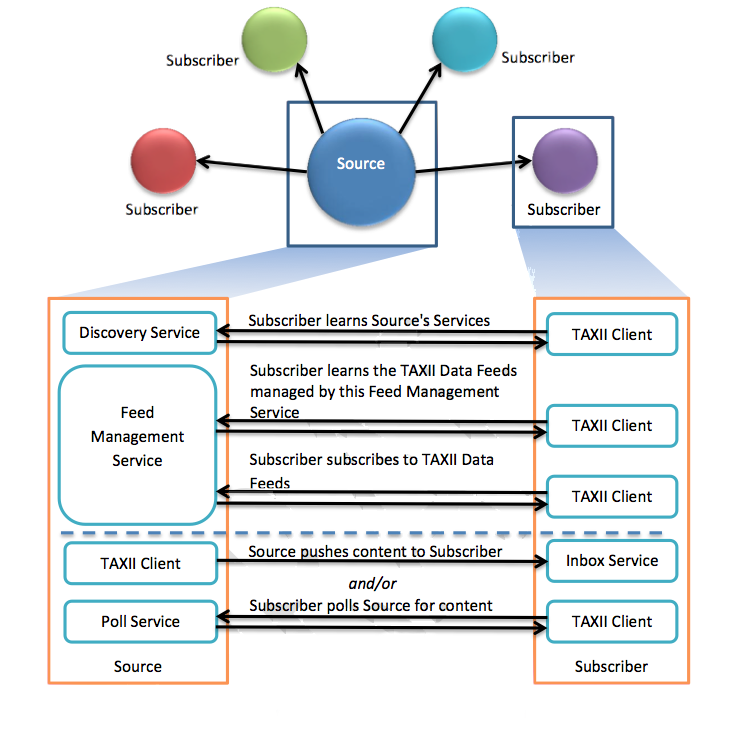
\includegraphics[width=150mm]{./images/SourceSuscriberModel.png}
    \caption{Flujo de información en modelo Source/Subscriber \protect\cite{b1}}
    \label{fig.sourcesuscribermodel}
\end{figure}

La figura \ref{fig.sourcesuscribermodel} muestra como el modelo Source/Subscriber puede ser soportado por los 
servicios TAXII. También se ven los mensajes TAXII intercambiados entre la
fuente y el subscriptor. Con los intercambios que están por encima de la línea 
punteada se establece la subscripción. Los intercambios pueden ser realizados 
repetidamente sin la necesidad de realizar el proceso de subscripción 
nuevamente.

\newpage

\paragraph{Peer-to-peer}\ \\ 

En un modelo Peer-to-peer, los pares de organizaciones entran en un acuerdo 
mutuo para compartir información entre si. En este modelo, cada Peer puede 
operar como productor y consumidor. Los socios en este intercambio podrían 
establecer fuentes utilizando un procedimiento similar al establecido en el 
modelo Source/Subscriber. Alternativamente, podrían acordar subir o descargar 
contenido sin ninguna subscripción formal. No tener una subscripción formal 
permite a un Peer albergar un Inbox Service sin necesidad de un Feed 
Managment Service.\\

El modelo Peer-to-Peer tiene dos variantes: acuerdos para el intercambio entre 
comunidades y acuerdos para el intercambio ad-hoc. En el primero la comunidad 
constituye acuerdos entre pares en los que todos los miembros acuerdan una única 
política la cual será respetada por todos. A diferencia de los otros dos 
modelos que tienen un punto central desde el cual la información es diseminada, 
todo el intercambio ocurre puntualmente entre dos pares. Si los pares A y B 
desean recibir información del peer C directamente, ambos necesitaran 
establecer un acuerdo apropiado con el peer C para que éste les envíe la 
información que desean.\\

Alternativamente, el intercambio entre pares puede ser realizado de forma 
individual con intercambios ad-hoc. Esto podría ocurrir si dos compañías hacen 
acuerdos individuales para compartir entre ellas. En este caso, los acuerdos 
sobre que compartir son específicos para las partes. Una sola entidad podría 
participar en ambas variantes, perteneciendo a una o mas comunidades en las 
cuales los miembros comparten entre si siguiendo un acuerdo común entre los 
miembros y a su vez negocian acuerdos individuales con otras entidades. Alguna 
información recibida por medio de un acuerdo no siempre debería ser compartida 
con otros pares que no son parte del acuerdo. De esta forma un participante 
debería hacer un seguimiento de quien fue el proveedor de la información 
recibida, como se realiza ese seguimiento está por fuera de la especificación de 
TAXII.\\

\begin{figure}[ht!]
  \centering
  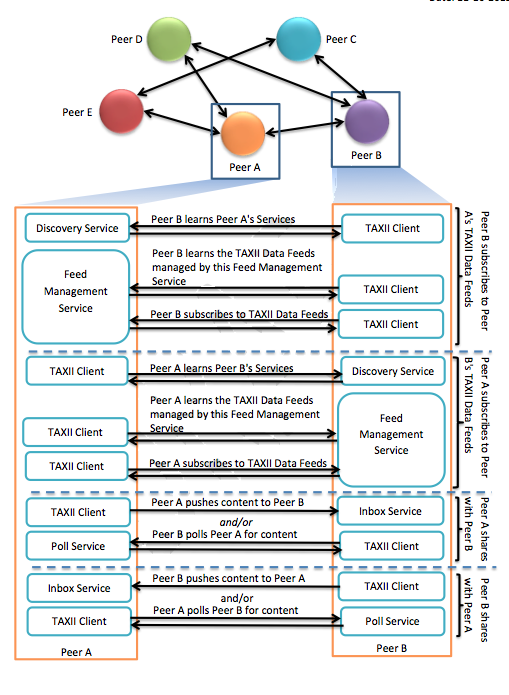
\includegraphics[scale=0.55]{./images/PeerToPeerModel.png}
    \caption{Flujo de información en modelo Peer to Peer \protect\cite{b1}}
  \label{fig.peertopeermodel}
\end{figure}

La figura \ref{fig.peertopeermodel} muestra como el modelo Peer to peer puede ser realizado por 
medio de los servicios TAXII. En este diagrama se ve que dos pares se contactan 
para pedir subscripciones para obtener información. Se asume que ambos pares 
tienen un Feed Managment Service que es utilizado para manejar todos los 
pedidos de subscripción.
\newpage

\paragraph{Hub and Spoke}\ \\

En un modelo Hub and Spoke, la entidad Hub es un consumidor de 
información que le proveen las entidades Spoke, pero a su vez se comporta como
un productor que brinda información a entidades 
Spoke. Una entidad Spoke podría ser un productor, dando información al Hub, un 
consumidor que reciba actualizaciones del Hub o ambas. El Hub puede utilizar un 
Inbox Service para recibir información de cualquiera que desee enviar 
información de forma voluntaria y/o podría requerir información de ciertas 
fuentes para guardar la información en una única ubicación. Desde este punto, el 
Hub puede funcionar como una entidad Source del modelo Source/Subscriber 
mientras que los Spoke serían Subscribers de dicho modelo. El Hub puede adoptar 
cualquier política respecto de la información que recibe, desde pasar toda la 
información automáticamente a solo pasar información de socios reconocidos, o 
realizar ediciones y análisis antes de reenviar la información.

\begin{figure}[ht!]
  \centering
    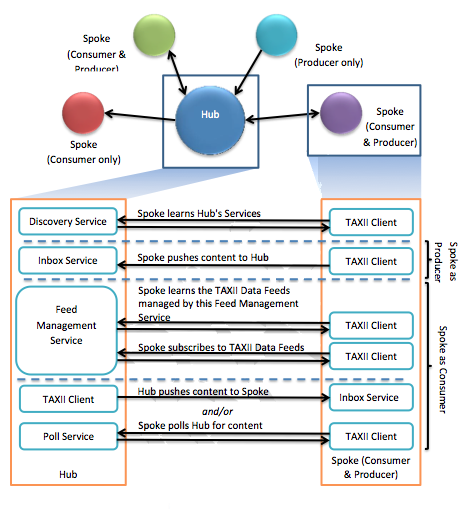
\includegraphics[scale=0.75]{./images/HubAndSpokeModel.png}
    \caption{Flujo de información en modelo Hub and Spoke \protect\cite{b1}}
    \label{fig.hubandspokemodel}
\end{figure}

La figura \ref{fig.hubandspokemodel} muestra como se puede implementar el modelo Hub and Spoke 
utilizando los servicios provistos por TAXII. En este modelo algunas entidades 
Spoke podrían ser consumidores, otras productores y en algunos casos ambas. El 
diagrama muestra los intercambios que podrían ser utilizados por el Spoke que 
actúa como productor y consumidor. Si este desea actuar de una sola forma solo 
los intercambios necesarios serían relevantes. Independientemente del rol que 
tome el Spoke, es necesario que éste conozca los servicios relevantes en el Hub. 
Esto se realiza utilizando el Discovery Service provisto por el Hub, de todas 
formas esto podría realizarse con mecanismos fuera de banda.



 

\setlength\tabcolsep{1mm}
\renewcommand\arraystretch{1.3}
\newcounter{Figura}
\renewcommand\theFigura{\arabic{Figura}}
\newcounter{Tabla}
\renewcommand\theTabla{\arabic{Tabla}}

\chapter{Análisis}
\label{capitulo2}
	
	A continuación se presentan los aspectos más importantes que se tuvieron en cuenta para el desarrollo del proyecto. Se
	presentan características deseadas en un sistema de intercambio de información de seguridad entre organizaciones.

\section{Análisis de requerimientos}
	Existen distintos problemas que obstaculizan el intercambio de información entre las organizaciones. Dichas
	problemáticas afectan la reputación, seguridad y la capacidad de trabajo de las organizaciones. \\

	Las organizaciones pueden intercambiar grandes volúmenes de datos los cuales pueden provenir de diferentes fuentes, cada
	una de estas fuentes puede utilizar una representación propia para los datos. Esto puede generar problemas para interpretar infromación proveniente de otra organización, y por ello es deseado que las
	organizaciones utilicen un estándar aceptado por todas. La representación utilizada debería permitir el desarrollo de
	herramientas que ayuden en la estructuración de los datos de forma de facilitar el trabajo de los
	analistas.\\

	Otro de los problemas que interfieren en el intercambio de información es el riesgo a la seguridad y reputación de la
	organización. La información intercambiada debe pasar por procesos que controlen los datos que se intercambien evitando
	de esta manera la divulgación de información sensible o privada.\\

	Estas son algunas de las problemáticas que se pueden identificar referentes al intercambio de información de seguridad.
	También existen otros problemas, como por ejemplo establecer un criterio referente a políticas organizacionales que
	ayuden a identificar organizaciones de confianza. Este problema no será analizado en este documento.\\


\bigskip

	La herramienta que se desea desarrollar busca ayudar a las organizaciones a solucionar algunos de los problemas
	planteados anteriormente y que afectan el intercambio de información con sus pares. Además es deseado que la
	herramienta pueda ser extendida en un futuro con nuevas funcionalidades que solucionen otras problemáticas no
	identificadas o que no se desarrollen en el transcurso de este proyecto.


\bigskip

	Se desea desarrollar una herramienta que se integre con alguna de las aplicaciones de gestión de incidentes existentes,
	proveyéndole así la capacidad de intercambiar información de seguridad. Dicha herramienta debería estructurar y organizar
	la información de forma de facilitar el intercambio. Además se debería dar la posibilidad de correlacionar la
	información de forma de facilitar el trabajo de los analistas. Una funcionalidad importante en una herramienta de estas
	características es la sanitiziación de los datos compartidos, con el fin de proteger la integridad de la organización
	durante los intercambios.


\bigskip

	Los intercambios podrían proveer información sobre la identificación de nuevas vulnerabilidades o entidades maliciosas,
	soluciones a problemas, prevención de problemas, etc. 


\bigskip

	El intercambio de información no es un problema estrictamente técnico, hay procedimientos y consideraciones legales y de
	confianza que podrían afectar el intercambio de información entre organizaciones. Durante el estado del arte se
	investigaron distintos protocolos y lenguajes para la representación de la información, se llegó a la conclusión \ de
	que ninguno de estos daba soluciones referentes a las políticas organizacionales que solucionaran problemas como la
	confianza entre las organizaciones o la información que debe ser compartida.


\bigskip

	A pesar de lo mencionado anteriormente, es deseable que un sistema que comparta información de seguridad respete y
	aplique las políticas organizacionales. Por ello es necesario que el sistema aplique políticas definidas por los
	administradores para sanitizar y anonimizar la información con el fin de remover datos confidenciales o sensibles antes
	de que sean compartidos. Para resolver este problema se debe evaluar la protección que se le quiere dar a la
	información y considerar a su vez cuan útil es dicha información luego de ser sanitizada.\\

	Del análisis anterior se desprende la necesidad de contar con un módulo que permita a la aplicación sanitizar la
	información. Como se mencionó anteriormente, los administradores definen dichas políticas en el sistema. La finalidad
	del módulo es analizar la información y filtrar datos que pudieran ser sensibles y que pusieran en riesgo los intereses
	de la organización.


\bigskip

	Durante el intercambio de información, se pueden obtener datos provenientes de diversas fuentes que se refieren a
	distintos tipos de información, pero que guarden una relación entre ellos. Por ello es necesario contar con un módulo
	que se encargue de relacionar la información por medio de la aplicación de estrategias. El resultado de la aplicación
	de estrategias es la agrupación de los datos, dicha agrupación permite a los analistas manejar una menor cantidad de
	datos y de esta forma simplificar su trabajo. Esto ayuda a bajar el periodo de tiempo entre la detección del problema y
	su solución.\\

	Con la correlación es posible vincular información generada por distintas fuentes para decidir si se tratan de falsos
	positivos o hechos reales. A su vez, permite detectar ataques que pudieran pasar desapercibidos en volúmenes muy
	grandes de información.\\

	Si bien la información correlacionada es de utilidad para los analistas, es necesario contar con toda la
	información recibida para poder hacer un análisis de los datos originales por parte de los analistas.


\bigskip

	Además de recibir información proveniente de otras organizaciones, es deseable que se pueda ingresar nueva información
	al sistema. Dicho ingreso de información se pretende realizar por medio del sistema de gestión de incidentes, a su vez
	se desea mantener una representación estructurada de la información ingresada en el incidente. Mantener la información
	de forma estructurada permite realizar la correlación con datos recibidos de otra organización. Esto permitiría por
	ejemplo ayudar a solucionar un problema para el cual otra organización tenga una solución.


\bigskip
\newpage
	De lo anterior se pueden identificar los siguientes requerimientos funcionales:
\begin{flushleft}
	\tablefirsthead{}
	\tablehead{}
	\tabletail{}
	\tablelasttail{}
	\begin{supertabular}{|m{5.83516in}|}
		\hline
		\begin{center}{\bfseries Requerimientos funcionales}
		\end{center}
		\\\hline
		\begin{itemize}
			\item {La herramienta debe implementar un modelo peer-to-peer de intercambio de
				información entre organizaciones.}
			\item {Se debe dar la posibilidad de sanitizar la información intercambiada por medio
				de políticas definidas por el administrador.}
			\item {Es deseable contar con un módulo para correlacionar la información de los
				incidentes configurable por el administrador.}
			\item {Dar la posibilidad de gestionar información de seguridad.}
		\end{itemize}
		\\\hline
	\end{supertabular}
\end{flushleft}
{\centering\selectlanguage{english}\bfseries
	\foreignlanguage{spanish}{Tabla }\stepcounter{Tabla}{\theTabla}\foreignlanguage{spanish}{ - Requerimientos funcionales
		del sistema.}
	\par}
\bigskip
	También se pueden ver los siguientes requerimientos no funcionales:

\begin{flushleft}
	\tablefirsthead{}
	\tablehead{}
	\tabletail{}
	\tablelasttail{}
	\begin{supertabular}{|m{5.83516in}|}
		\hline
		\begin{center}{\bfseries Requerimientos no funcionales}
		\end{center}
		\\\hline
		\begin{itemize}
			\item {Extensibilidad: Debe ser posible extender la herramienta con nuevos módulos que
				implementen nuevas funcionalidades.}
			\item {Independencia del sistema de gestión de incidentes para que exista la posibilidad de
				utilizar otra herramienta.}
		\end{itemize}
		\\\hline
	\end{supertabular}
\end{flushleft}
{\centering\selectlanguage{english}\bfseries
	\foreignlanguage{spanish}{Tabla }\stepcounter{Tabla}{\theTabla}\foreignlanguage{spanish}{ - Requerimientos no
		funcionales del sistema.}
	\par}


\bigskip

\section{Herramientas}
	En esta sección se muestran las herramientas utilizadas. STIX fue elegida porque provee una representación estructurada
	y estándar de la información. Junto con STIX se eligió TAXII el cual ha sido diseñado para intercambiar información de
	seguridad representada por medio del lenguaje STIX y que tiene consideraciones para realizar el intercambio.
	Posteriormente se menciona a que se debió la utilización de RTIR y se detalla en mayor profundidad la selección de STIX
	y TAXII.\\
	\bigskip

	Además se consideraron en menor medida la posibilidad de desarrollar trabajo futuro con dichas herramientas y su
	aceptación por parte de la comunidad.


\bigskip

\subsection{RTIR}

\bigskip

	RTIR es un sistema de manejo de incidentes diseñado para ser utilizado por \ CSIRTs para manejar el creciente número de
	incidentes reportados. Si bien existen otras herramientas similares, RTIR presenta la ventaja de ser
	\textit{opensource} y contar con una API que permite extender la herramienta de forma sencilla. También es posible
	desarrollar \textit{plugins} para extender las funcionalidades de la herramienta. RTIR cuenta además con una comunidad
	de usuarios grande cuya característica principal es el nivel técnico de estos.\\
	\bigskip

	Distintos CSIRTs han contribuido en el desarrollo de la herramienta, el resultado ha sido una herramienta que posee un
	\textit{workflow} para el manejo de incidentes de seguridad. Dicho \textit{workflow} facilita el trabajo de los
	CSIRTs.\\
\bigskip
	Como se mencionó en el capítulo 2, RTIR no cuenta con una representación estructurada de la información ni tampoco
	con un método automático para compartir información de seguridad. Una integración con TAXII y STIX le permitiría cubrir
	estas dos falencias.


\bigskip

	El interés de usar RTIR proviene de que el CSIRT-Tilsor \ tiene la herramienta instalada y la utiliza para sus
	operaciones. Además hay miembros del equipo que tienen experiencia en su uso.


\bigskip

	Además, al ser una herramienta con una profunda inserción en la comunidad, es esperable que sea más fácil la aceptación
	de una extensión basada en TAXII y STIX que la creación de una nueva herramienta a la que los usuarios deberán
	adaptarse.


\bigskip

	Si bien RTIR fue una premisa dentro de los objetivos del proyecto, se evaluaron durante el estudio del arte otras
	herramientas que pudieran tomar su lugar. De todas formas, del análisis realizado, se eligió RTIR por las razones dadas
	anteriormente. A pesar de utilizarse RTIR, es deseable que la herramienta desarrollada no sea dependiente de RTIR, esto
	quiere decir que se pueda utilizar una herramienta con funcionalidades similares en el futuro.

\subsection{STIX y TAXII}

\bigskip

	Se decidió utilizar STIX para representar la información por la facilidad con la que permite representar información de
	seguridad de forma estructurada y estándar. Por medio de CybOX se permite describir evidencia en la forma de
	observables, artefactos y/o comportamientos presentes en un sistema. La representación de forma precisa se debe a la
	gran gama de objetos distintos que permite describir, entre ellos, el nombre de procesos ejecutándose, hash de archivos
	o mensajes ICMP. Como se vio en el estado del arte, STIX también permite representar incidentes, tácticas, técnicas y
	procedimientos de los adversarios, actores maliciosos entre otros conceptos que permiten representar adecuadamente
	información de seguridad.


\bigskip

	Otras de las características que posee STIX son la extensibilidad, la simpleza y la facilidad de procesamiento. Dichas
	características son propias de un lenguaje XML.


\bigskip

	TAXII define un conjunto de servicios e intercambios de mensajes que permiten el intercambio de información de
	seguridad. En la especificación de TAXII se establece que la información de seguridad es representada por medio de
	STIX. Además TAXII posee consideraciones de seguridad para realizar el intercambio como lo son encriptación y
	autenticación.


\bigskip

	TAXII realiza el intercambio de conjuntos de información de seguridad llamados ``TAXII Data Collections''. Dichas
	colecciones de datos pueden ser conjuntos ordenados de información (``TAXII Data Feeds'') en los cuales el criterio de
	ordenación es un \textit{timestamp} o conjuntos desordenados (``TAXII Data Sets''). La información en dichos conjuntos
	es representada de forma estructurada utilizando el lenguaje STIX. Durante los intercambios de información es necesario
	que el cliente pida información de una de las colecciones de las que dispone el productor. Por ello es necesario que se
	de en el sistema la posibilidad de gestionar las colecciones a las que un cliente se suscribe.


\bigskip

	\ \ STIX también integra con otras iniciativas de MITRE e incluso se integra con lenguajes de otras organizaciones como
	IODEF de IEEE y OpenIOC de Mandiant.


\bigskip

	Es importante mencionar que STIX ha tenido un fuerte apoyo de la comunidad y busca convertirse en un estándar. Actualmente
	existen esfuerzos para crear herramientas que utilicen el lenguaje STIX y que realice un intercambio \ de información
	por medio de TAXII.

\bigskip

	Con las herramientas mencionadas anteriormente podemos ver un diagrama de bloques como el de la figura \ref{fig.diagramabloques}. En la figura
	se puede ver que se cuenta con una instalación de la herramienta RTIR que será la encargada de la gestión de incidentes
	y por medio de la cual se dará de alta la información en el sistema. Además en el bloque ``TAXII App'' realiza el
	intercambio de información con otras organizaciones por medio de TAXII y representa la información utilizando STIX.
	Además dicho bloque es el encargado de realizar la sanitización y correlación de información.

\begin{figure}[h!]
	\centering
	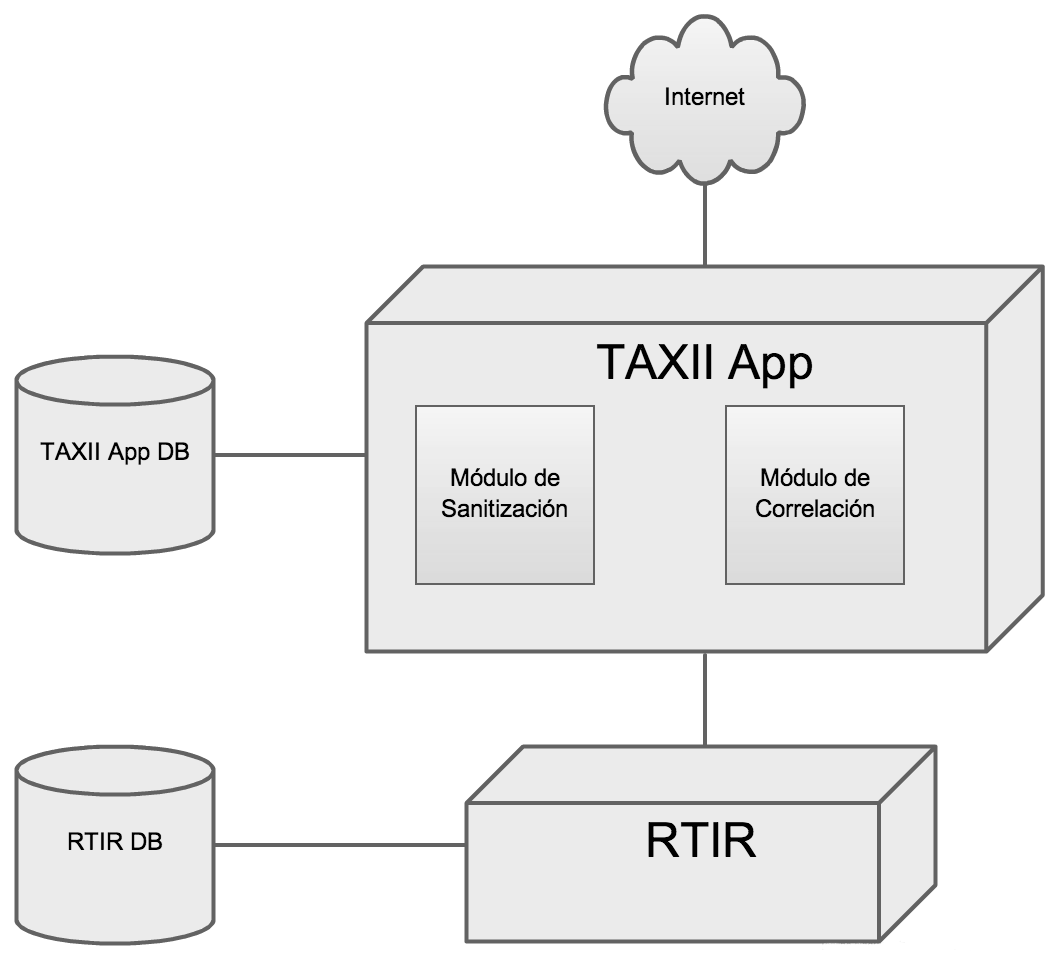
\includegraphics[width=1.9673in,height=1.7811in]{Analisis22-img/Analisis22-img016.png}
	\caption{Diagrama de Bloques del sistema}
	\label{fig.diagramabloques}
\end{figure}

\bigskip


\bigskip

\section{Actores y Casos de Uso}
\subsection{Actores}

\bigskip

\begin{flushleft}
	\tablefirsthead{}
	\tablehead{}
	\tabletail{}
	\tablelasttail{}
	\begin{supertabular}{m{0.8608598in}m{4.89486in}}
		{Actor} &
		{Analista}\\\hline
		\multicolumn{1}{m{0.8608598in}|}{{Descripción}} &
		\multicolumn{1}{m{4.89486in}|}{{Este actor tiene la posibilidad de ingresar nueva
				información en el sistema. Dicha información puede ser intercambiada con otro sistema. Con la información que se ha
				intercambiado el actor puede realizar un análisis de ella y hacer un manejo de los casos creados en el RTIR.}}\\
	\end{supertabular}
\end{flushleft}

\bigskip
\bigskip
\bigskip

\begin{flushleft}
	\tablefirsthead{}
	\tablehead{}
	\tabletail{}
	\tablelasttail{}
	\begin{supertabular}{m{0.8816598in}m{4.8740597in}}
		{Actor} &
		{Cliente TAXII}\\\hline
		\multicolumn{1}{m{0.8816598in}|}{{Descripción}} &
		\multicolumn{1}{m{4.8740597in}|}{{Este actor es el que interactúa con el sistema
				para intercambiar datos por medio del protocolo TAXII. El sistema tiene que dar soporte para dicho protocolo para que
				el intercambio sea exitoso.}}\\
	\end{supertabular}
\end{flushleft}

\bigskip

\subsection{Casos de uso y diagramas de secuencia}

\bigskip

\subsubsection{ABM de políticas de sanitización}
\begin{flushleft}
	\tablefirsthead{}
	\tablehead{}
	\tabletail{}
	\tablelasttail{}
	\begin{supertabular}{m{1.0573599in}|m{4.82056in}|}
		\multicolumn{1}{m{1.0573599in}}{{Nombre}} &
		\multicolumn{1}{m{4.82056in}}{{ABM de políticas de sanitización}}\\\hline
		{Actor} &
		{Analista}\\
		{Descripción} &
		{Estos casos de uso comienzan cuando el analista desea realizar el alta, baja o
			modificación de las políticas de sanitización. Por medio de estas se filtra la información que se desea intercambiar
			con otras organizaciones.}\\\hhline{~-}
	\end{supertabular}
\end{flushleft}

\bigskip

{
	\bigskip
	En la figura \ref{fig.altasanitizacion} se especifica el caso de uso, en este un analista ingresa a RTIR y da de alta en el sistema una política
	de sanitización. Dicha política es utilizada para realizar la sanitización de la información intercambiada por la
	organización. Las políticas son registradas en TAXII App.}
\bigskip
\begin{figure}[ht!]
	\centering
	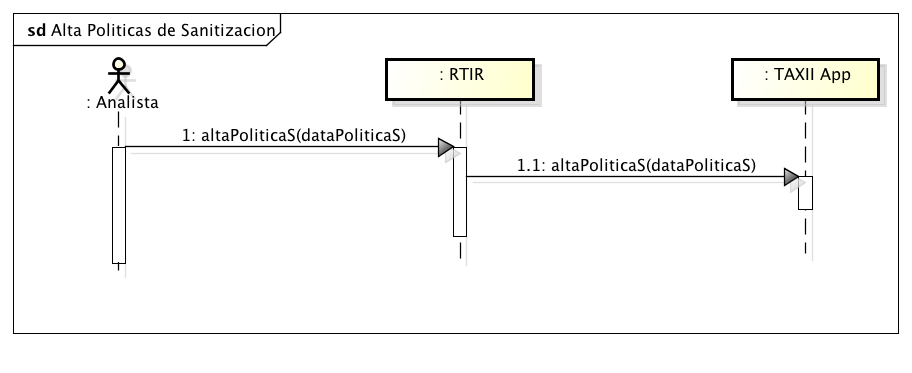
\includegraphics[width=5.7638in,height=2.3575in]{Analisis22-img/Analisis22-img017.png} 
	\caption{Caso de Uso alta políticas de sanitización}
	\label{fig.altasanitizacion}
\end{figure}

\begin{figure}[ht!]
	\centering
	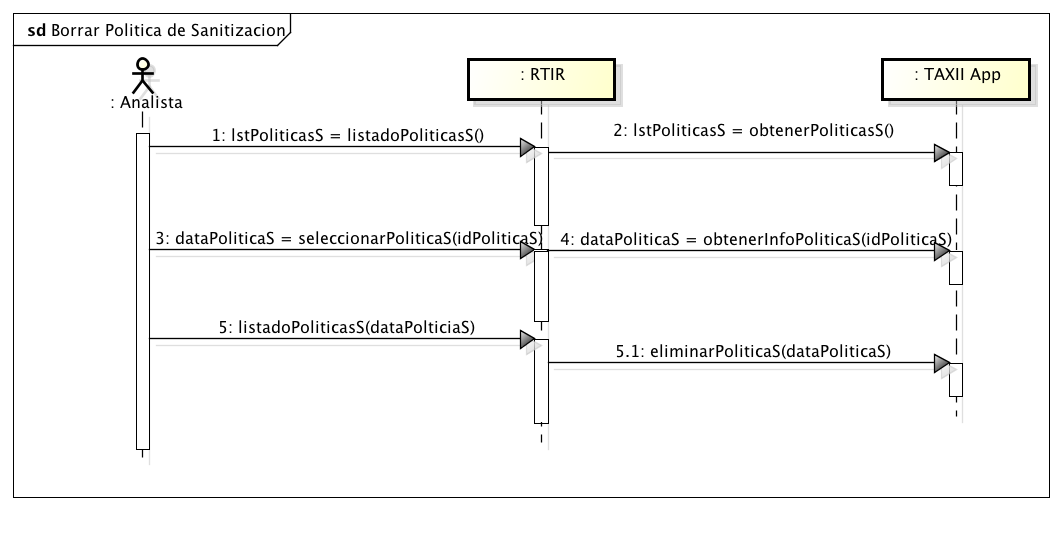
\includegraphics[width=5.7638in,height=2.9146in]{Analisis22-img/Analisis22-img018.png} 
	\caption{Caso de uso borrado políticas de sanitización}
	\label{fig.borradosanitizacion}
\end{figure}

\bigskip

	En la figura \ref{fig.borradosanitizacion} se especifica el caso de uso de borrado de políticas de sanitización, en este un analista ingresa a RTIR
	y lista todas las políticas disponibles en el sistema. Luego selecciona la política que desea dar de baja para luego
	borrarla.


\newpage
\begin{figure}[ht!]
	\centering
	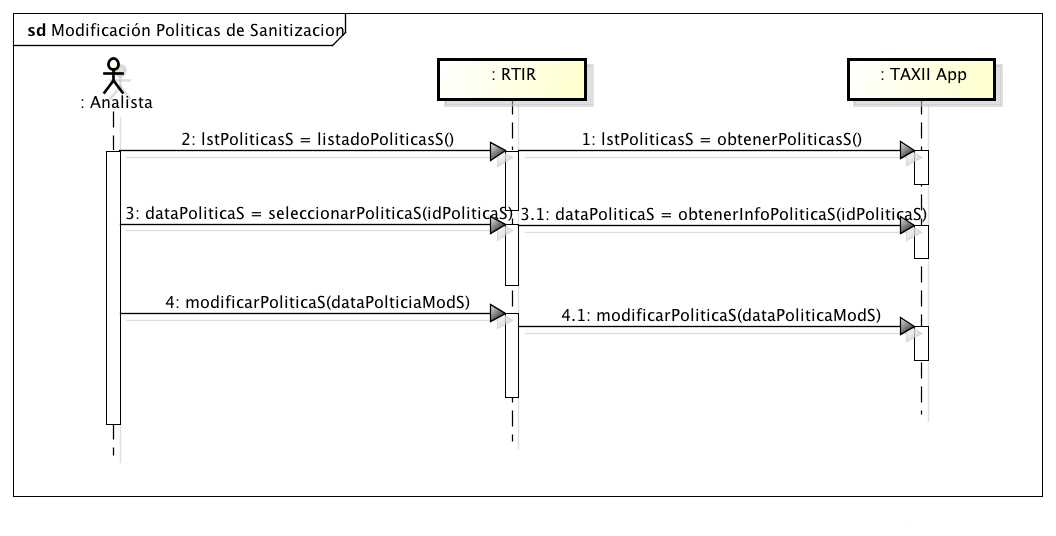
\includegraphics[width=5.7638in,height=2.9256in]{Analisis22-img/Analisis22-img019.png} 
	\caption{Caso de uso modificación de políticas de sanitización}
	\label{fig.modificacionsanitizacion}
\end{figure}
\bigskip
	En la figura \ref{fig.modificacionsanitizacion} se especifica el caso de uso de modificación de políticas de sanitización, en este un analista ingresa a
	RTIR y lista todas las políticas disponibles en el sistema. Luego selecciona la política que desea modificar.
\newpage
\subsubsection{ABM de Políticas de Correlación}
\begin{flushleft}
	\tablefirsthead{}
	\tablehead{}
	\tabletail{}
	\tablelasttail{}
	\begin{supertabular}{m{1.0573599in}|m{4.82056in}|}
		\multicolumn{1}{m{1.0573599in}}{{Nombre}} &
		\multicolumn{1}{m{4.82056in}}{{ABM de políticas de correlación}}\\\hline
		{Actor} &
		{Analista}\\
		{Descripción} &
		{Estos casos de uso comienzan cuando el analista desea realizar el alta, baja o
			modificación de las políticas de correlación. Por medio de estas se agrupa la información según los datos existentes en
			el sistema.}\\\hhline{~-}
	\end{supertabular}
\end{flushleft}

\bigskip
\begin{figure}[ht!]
	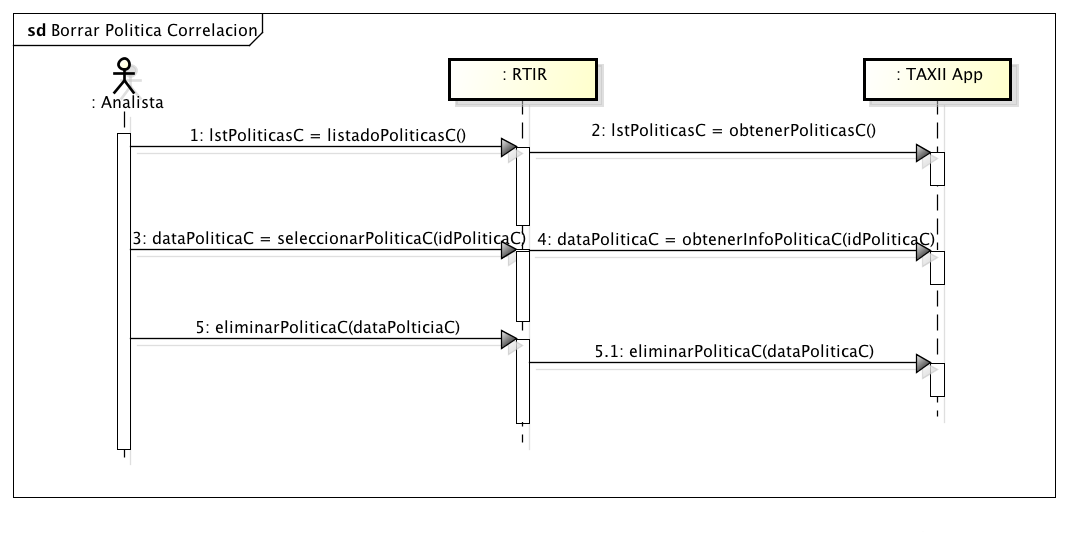
\includegraphics[width=5.7634in,height=2.898in]{Analisis22-img/Analisis22-img020.png}
	\caption{Caso de uso borrado políticas de correlación} 
	\label{fig.borradocorrelacion}
\end{figure}

	En la figura \ref{fig.borradocorrelacion} se especifica el caso de uso de borrado de políticas de correlación, en este un analista ingresa a RTIR y
	lista todas las políticas disponibles en el sistema. Luego selecciona la política que desea dar de baja para luego
	borrarla.


\bigskip


\bigskip
\begin{figure}[ht!]
	\centering
	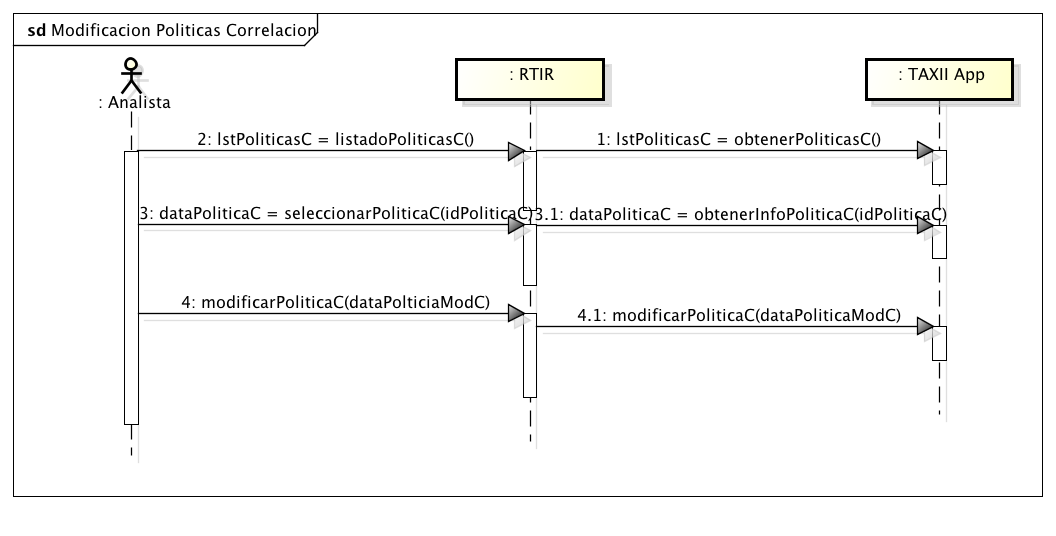
\includegraphics[width=5.7638in,height=2.9256in]{Analisis22-img/Analisis22-img021.png} 
	\caption{Caso de uso modificación políticas de correlación}
	\label{fig.modificacioncorrelacion}
\end{figure}
	En la figura \ref{fig.modificacioncorrelacion} se especifica el caso de uso de modificación de políticas de correlación, en este un analista ingresa a
	RTIR y lista todas las políticas disponibles en el sistema. Luego selecciona la política que desea modificar.


\bigskip
\begin{figure}[ht!]
	\centering
	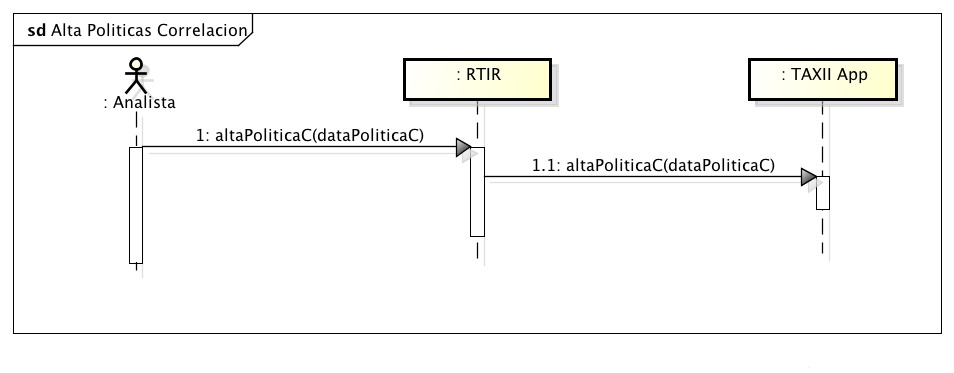
\includegraphics[width=5.7638in,height=2.2535in]{Analisis22-img/Analisis22-img022.png} 
	\caption{Caso de uso alta políticas de correlación}
	\label{fig.altacorrelacion}
\end{figure}
	En la figura \ref{fig.altacorrelacion} se especifica el caso de uso de alta de políticas de correlación, en este un analista ingresa a RTIR y
	da de alta en el sistema una política de correlación. Dicha política es utilizada para realizar la correlación de la
	información presente en el sistema. Las políticas son registradas en TAXII App.


\newpage

\subsubsection{ABM de Servicios TAXII}

\bigskip

\begin{flushleft}
	\tablefirsthead{}
	\tablehead{}
	\tabletail{}
	\tablelasttail{}
	\begin{supertabular}{m{1.0573599in}|m{4.82056in}|}
		\multicolumn{1}{m{1.0573599in}}{{Nombre}} &
		\multicolumn{1}{m{4.82056in}}{{ABM de servicios TAXII}}\\\hline
		{Actor} &
		{Analista}\\
		{Descripción} &
		{Estos casos de uso comienzan cuando el analista desea realizar el alta, baja o
			modificación de servicio TAXII de otras organizaciones en el sistema. Estos serán utilizados para lograr el intercambio
			de información.}\\\hhline{~-}
	\end{supertabular}
\end{flushleft}

\bigskip

\begin{figure}[ht!]
	\centering
	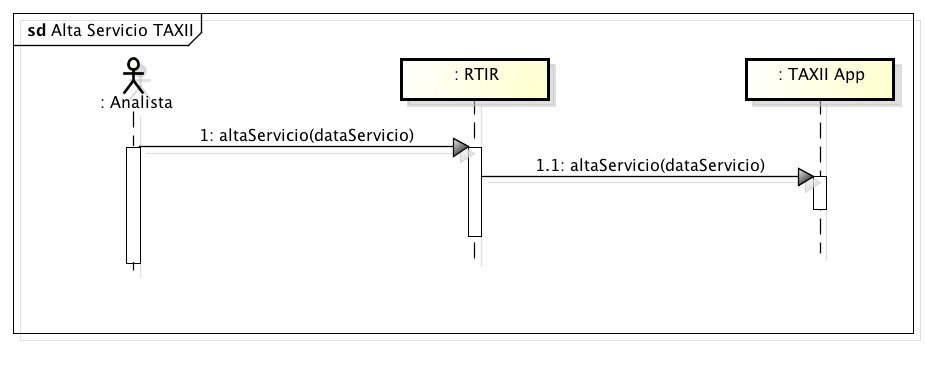
\includegraphics[width=5.7638in,height=2.3217in]{Analisis22-img/Analisis22-img023.png} 
	\caption{Caso de uso alta servicio TAXII}
	\label{fig.altaserviciotaxii}
\end{figure}
	En la figura \ref{fig.altaserviciotaxii} se especifica el caso de uso de alta de servicios TAXII, en este un analista ingresa a RTIR y da de alta
	en el sistema un servicio TAXII. Por medio de dicho servicio se realizara el intercambio con otra organización.


\bigskip
\begin{figure}[ht!]
	\centering
	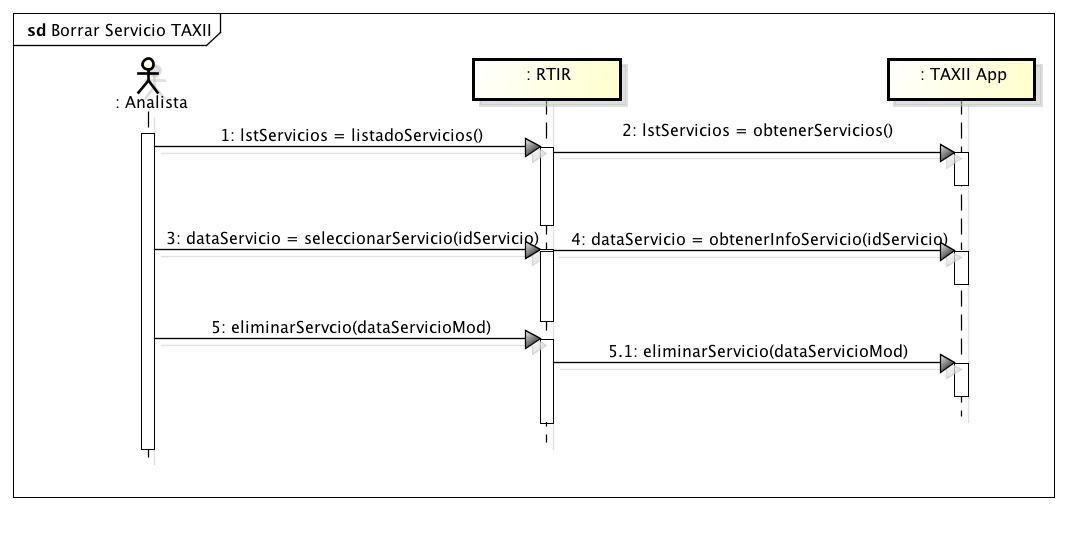
\includegraphics[width=5.7634in,height=2.898in]{Analisis22-img/Analisis22-img024.png} 
	\caption{Caso de uso borrar	servicio TAXII}
	\label{fig.borradoserviciotaxii}
\end{figure}
	En la figura \ref{fig.borradoserviciotaxii} se especifica el caso de uso de borrado de servicios TAXII, en este un analista ingresa a RTIR y lista
	todas las servicios disponibles en el sistema. Luego selecciona el que desea dar de baja.
\newpage
\begin{figure}
	\centering
	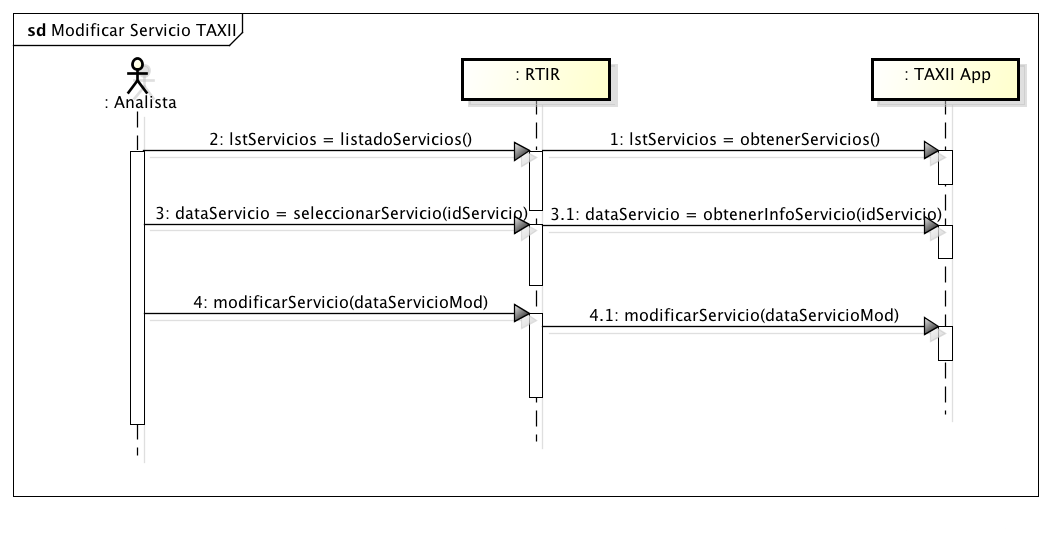
\includegraphics[width=5.7638in,height=2.9366in]{Analisis22-img/Analisis22-img025.png} 
	\caption{Caso de uso modificar servicio TAXII}
	\label{fig.modificarserviciotaxii}
\end{figure}

	En la figura \ref{fig.modificarserviciotaxii} se especifica el caso de uso de modificación de servicios TAXII, en este un analista ingresa a RTIR y
	lista todos los servicios disponibles. Luego selecciona el que será modificado.
\newpage
\subsubsection{Alta de información}

\begin{flushleft}
	\tablefirsthead{}
	\tablehead{}
	\tabletail{}
	\tablelasttail{}
	\begin{supertabular}{m{0.8816598in}|m{4.8740597in}|}
		\multicolumn{1}{m{0.8816598in}}{{Nombre}} &
		\multicolumn{1}{m{4.8740597in}}{{Alta de información RTIR}}\\\hline
		{Actor} &
		{Analista}\\
		{Descripción} &
		{Este caso de uso comienza cuando el analista desea registrar nueva información en
			el sistema. Es deseado que se pueda dar de alta información
			referente a cyber observables como por ejemplo IPs, hash de archivos, descripciones de amenazas, etc.}\\\hhline{~-}
	\end{supertabular}
\end{flushleft}

\begin{figure}
	\centering
	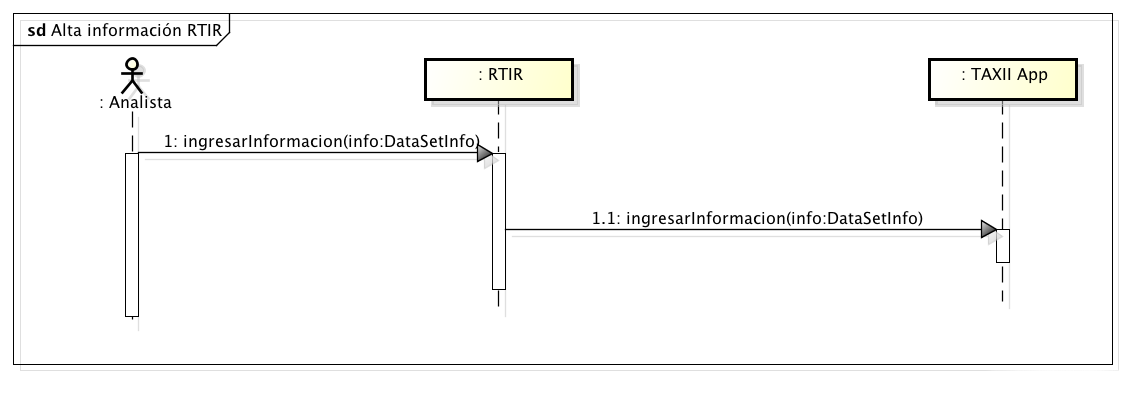
\includegraphics[width=5.7638in,height=2.0701in]{Analisis22-img/AltaInfoRTIR.png} 
	\caption{Caso de uso alta de información RTIR}
	\label{fig.altainfortir}
\end{figure}
\bigskip
	En la figura \ref{fig.altainfortir} se ve el caso de uso de alta de información en RTIR. En este un analista ingresa al sistema un cyber observable que será dado de alta en el sistema.En TAXII App se da de alta la información representando y
	almacenándola de forma estructurada por medio de STIX.


\newpage
\subsubsection{Asociación de información}

\begin{flushleft}
	\tablefirsthead{}
	\tablehead{}
	\tabletail{}
	\tablelasttail{}
	\begin{supertabular}{m{0.8816598in}|m{4.8740597in}|}
		\multicolumn{1}{m{0.8816598in}}{{Nombre}} &
		\multicolumn{1}{m{4.8740597in}}{{Asociación de información}}\\\hline
		{Actor} &
		{Analista}\\
		{Descripción} &
		{Este caso de uso comienza cuando el analista desea asociar contenido existente en TAXII App a un Ticket de RTIR. La información asociada al caso de RTIR puede ser utilizada durante la resolución de un incidente.}\\\hhline{~-}
	\end{supertabular}
\end{flushleft}

\begin{figure}
	\centering
	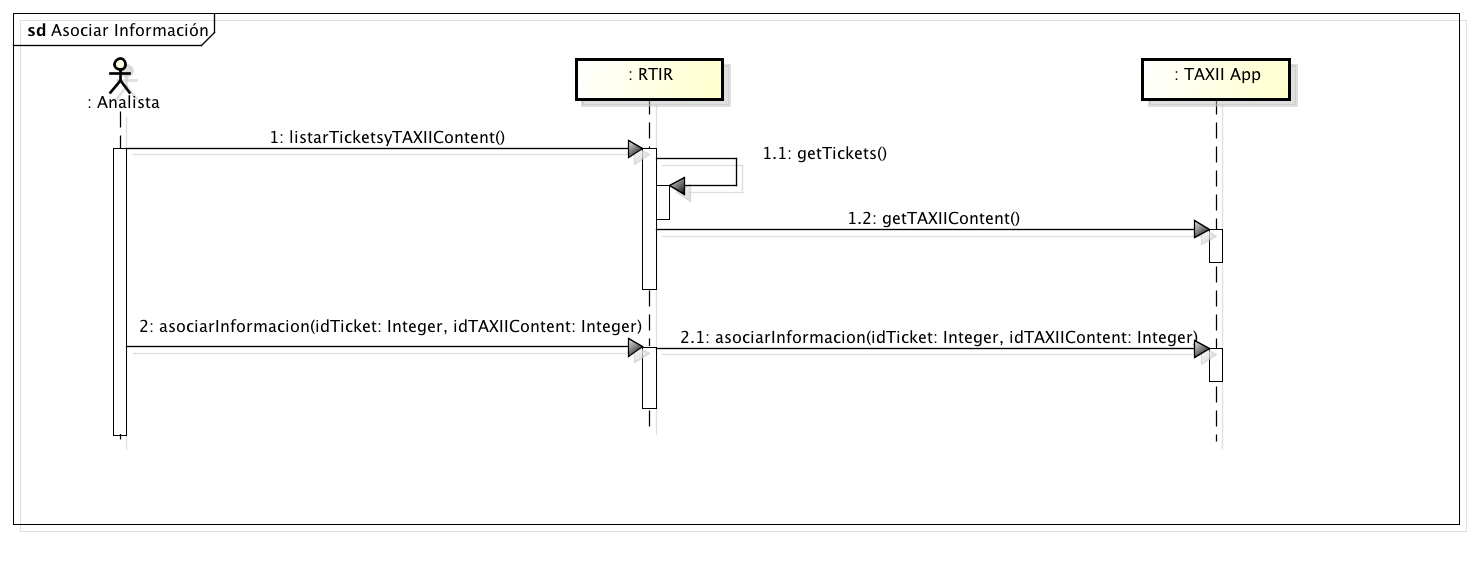
\includegraphics[width=5.7638in,height=2.0701in]{Analisis22-img/AsociacionInformacion.png} 
	\caption{Caso de uso asociación de información}
	\label{fig.asocinfortir}
\end{figure}
\bigskip
	En la figura \ref{fig.asocinfortir} se ve el caso de uso de asociación de información. En este un analista asocia un ticket existente en RTIR con información estructurada almacenada en TAXII App. Como se dijo anteriormente dicha información es almacenada utilizando STIX.

\newpage
\subsubsection{Subscripción a TAXII Data Feed}
\begin{flushleft}
	\tablefirsthead{}
	\tablehead{}
	\tabletail{}
	\tablelasttail{}
	\begin{supertabular}{m{0.8816598in}|m{4.8740597in}|}
		\multicolumn{1}{m{0.8816598in}}{{Nombre}} &
		\multicolumn{1}{m{4.8740597in}}{{Subscripción a Taxii
					Data Feed}}\\\hline
		{Actor} &
		{Analista}\\
		{Descripción} &
		{Con este caso de uso un analista selecciona un data feed en otro sistema al que
			quiere subscribirse. Esto se realiza por medio del Feed Managment Service de los sistemas.}\\\hhline{~-}
	\end{supertabular}
\end{flushleft}

\bigskip
\begin{figure}[ht!]
	\centering
	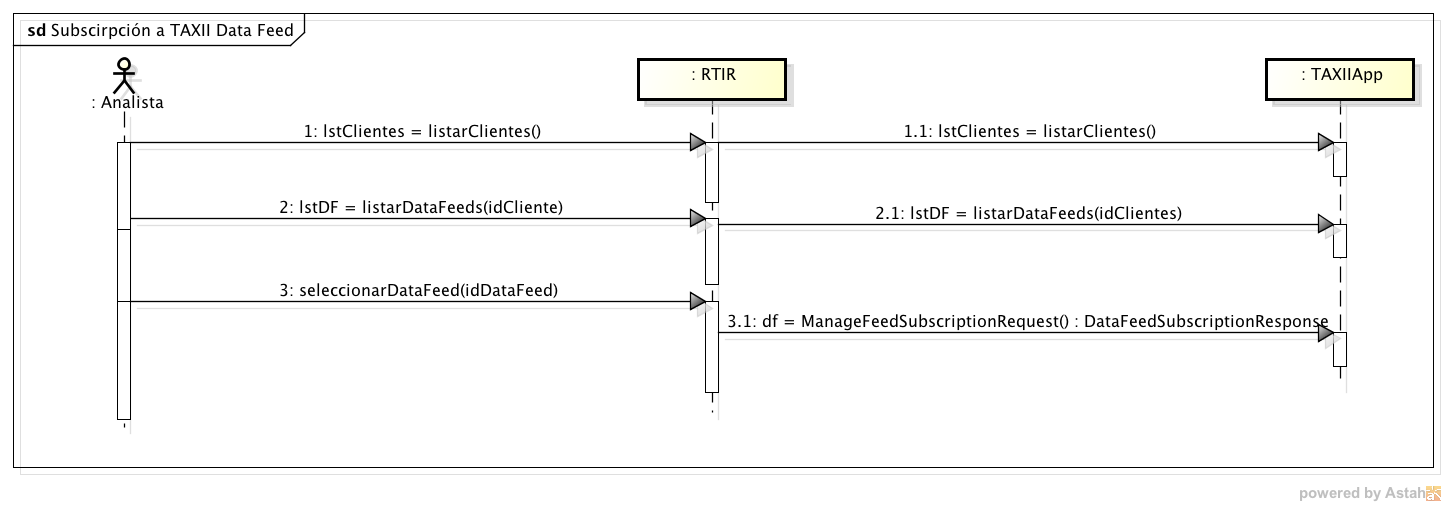
\includegraphics[width=5.4217in,height=1.8965in]{Analisis22-img/Analisis22-img027.png}
	\caption{Caso de uso subscripción a TAXII Data Feed}
	\label{fig.subscripciontaxiidatafeed}

\end{figure}

	En este caso de uso el analista desea subscribirse a uno de los TAXII data feed provistos por otra organización. Para
	ello obtiene un listado de los clientes TAXII con los que se relaciona para luego obtener un listado de los Data Feeds
	disponibles en ese cliente. Finalmente selecciona el TAXII data feed deseado.

\newpage
\subsubsection{Recepción de información}
\begin{flushleft}
	\tablefirsthead{}
	\tablehead{}
	\tabletail{}
	\tablelasttail{}
	\begin{supertabular}{m{0.8816598in}|m{4.8740597in}|}
		\multicolumn{1}{m{0.8816598in}}{{Nombre}} &
		\multicolumn{1}{m{4.8740597in}}{{Recepción de información}}\\\hline
		{Actor} &
		{Cliente TAXII}\\
		{Descripción} &
		{Este caso de uso se da cuando un cliente TAXII desea enviarle información a
			nuestro sistema. El envío de información se realiza porque un analista se subscribió a un data feed en el cliente. La
			recepción de información se realiza por medio del Inbox Service de nuestro sistema.}\\\hhline{~-}
	\end{supertabular}
\end{flushleft}
\begin{figure}[ht!]
	\centering
	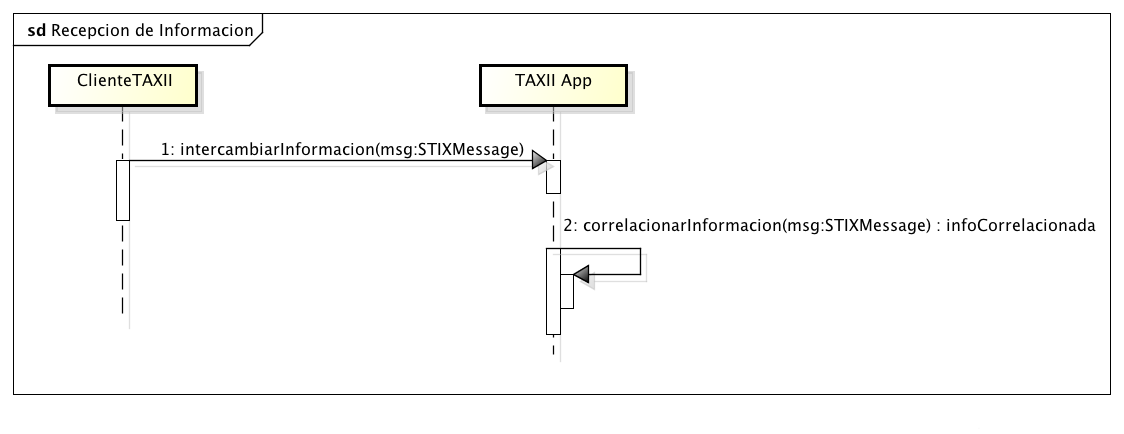
\includegraphics[width=5.7638in,height=2.2256in]{Analisis22-img/Analisis22-img028.png} 
	\caption{Caso de uso de recepción de información}
	\label{fig.recepcioninfo}
\end{figure}

	En este caso de uso un cliente TAXII en otra organización envía información a TAXII App. Luego la aplicación
	correlaciona la nueva información con la ya existente en el sistema.
\newpage
\subsubsection{Envío de información}
\begin{flushleft}
	\tablefirsthead{}
	\tablehead{}
	\tabletail{}
	\tablelasttail{}
	\begin{supertabular}{m{0.8816598in}|m{4.8740597in}|}
		\multicolumn{1}{m{0.8816598in}}{{Nombre}} &
		\multicolumn{1}{m{4.8740597in}}{{Envío de información}}\\\hline
		{Actor} &
		{TAXII App}\\
		{Descripción} &
		{Este caso de uso se da cuando el sistema desea enviar información a otro cliente
			TAXII. El envío de información se realiza porque el cliente se subscribió al TAXII Data Feed del sistema. Esto se
			realiza por medio del Inbox Service del cliente. El intercambio es iniciado por el sistema.}\\\hhline{~-}
	\end{supertabular}
\end{flushleft}
\begin{figure}[ht!]
	\centering  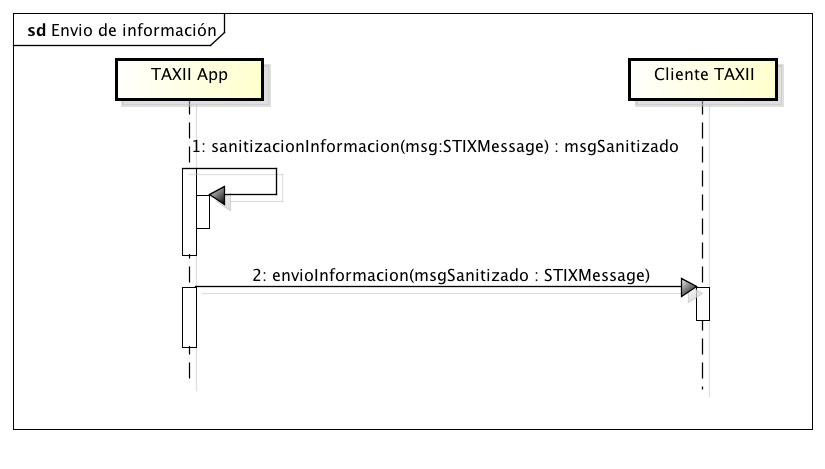
\includegraphics[width=5.7638in,height=3.2764in]{Analisis22-img/Analisis22-img029.png}
	\caption{Caso de uso de envío de información}
	\label{fig.enviodeinfo}
\end{figure}

	En este caso de uso TAXII App se comporta como el Actor y desea enviar nueva información a un cliente TAXII. Para ello
	lo primero que debe hacer es sanitizar la información. Luego envía la información representada en la forma de un
	mensaje STIX. Esto se ve en la figura \ref{fig.enviodeinfo}.
\newpage
\subsubsection{Poll de información}
\begin{flushleft}
	\tablefirsthead{}
	\tablehead{}
	\tabletail{}
	\tablelasttail{}
	\begin{supertabular}{m{0.8816598in}|m{4.8740597in}|}
		\multicolumn{1}{m{0.8816598in}}{{Nombre}} &
		\multicolumn{1}{m{4.8740597in}}{{Poll de información}}\\\hline
		{Actor} &
		{TAXII App}\\
		{Descripción} &
		{Este caso de uso se da cuando un cliente desea recibir información de un
			productor TAXII, en este los intercambios son iniciados por el cliente que contacta al Poll Service del
			productor.}\\\hhline{~-}
	\end{supertabular}
\end{flushleft}

\bigskip
\begin{figure}
	\centering  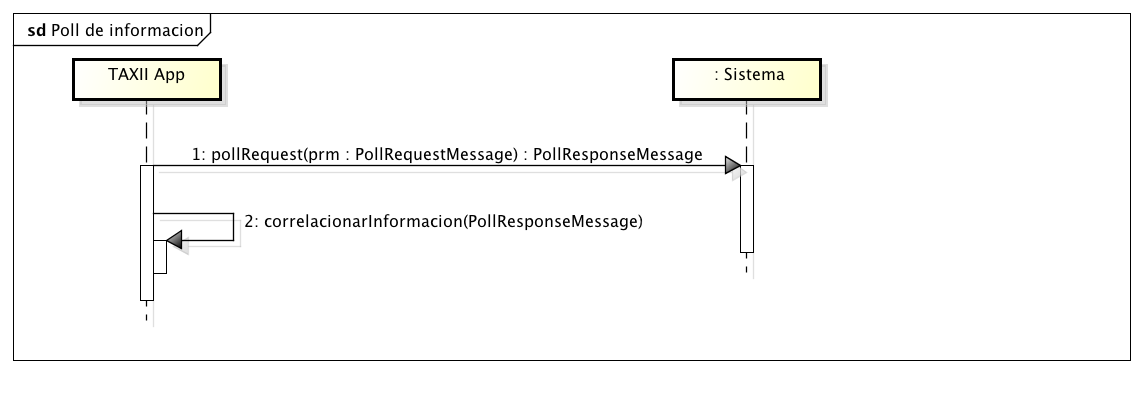
\includegraphics[width=5.7638in,height=2.0154in]{Analisis22-img/Analisis22-img030.png}
	\caption{Caso de uso de poll de
		información}
	\label{fig.pollinfo}
\end{figure}
	En la figura \ref{fig.pollinfo} se ve el caso de uso de poll de información. En este TAXII App realiza el pedido de información a otro
	cliente TAXII por medio de mensajes Poll Request. Cuando obtiene la información esta se correlaciona con los datos
	existentes en el sistema.


\bigskip


\bigskip

	También se deben considerar los casos de uso provistos por RTIR para el seguimiento y manejo de los incidentes los
	cuales no serán especificados en este documento ya que se pueden encontrar en \foreignlanguage{spanish}{[RTIR]}. Dichos
	casos de uso permiten el manejo de \textit{tickets}, \textit{queues }y gestión de usuarios.

	Con RTIR se especifica un \textit{workflow} para el trabajo con los \textit{tickets} en organizaciones de seguridad.
	Dicho \textit{workflow} comienza cuando se reporta un incidente, dicho reporte de incidente se asocia a un incidente o
	se crea uno nuevo. Los incidentes tratan de registrar toda la información necesaria para resolver el problema. De los
	incidentes se pueden iniciar investigaciones para trabajar con otras organizaciones. También se pueden crear
	\textit{blocks} para mantener un registro de las acciones realizadas para mitigar el incidente.

%\newpage en otro lado
%\nocite{*}
%\bibliographystyle{plain} 
%\bibliography{bibliography}

\makeatother
\setlength\tabcolsep{1mm}
\renewcommand\arraystretch{1.3}
\newcounter{FiguraCap4}
\renewcommand\theFigura{\arabic{FiguraCap4}}
\newcounter{TablaCap4}
\renewcommand\theTabla{\arabic{TablaCap4}}

\chapter{Diseño}
\label{capitulo4}
	En este capítulo se propone una solución que respeta los requerimientos que se especificaron
		durante el análisis. Además se describe el funcionamiento de la herramienta propuesta identificando los componentes que
		participan en dicho proceso. También se explica la arquitectura de la aplicación con la función de cada una de sus
		componentes. Finalmente se detalla el modelo de datos creado para la base de datos.
	
	\section[Contexto para el uso del sistema\ \ ]{\foreignlanguage{spanish}{Contexto para el uso del sistema\ \ }}
	\foreignlanguage{spanish}{Por medio del sistema propuesto es posible ingresar información de seguridad, correlacionarla
		con información existente en el sistema, y, luego de ser sanitizada, compartirla con organizaciones socias.}
	
	
	\bigskip
	
	\foreignlanguage{spanish}{El sistema ha sido diseñado para que sea utilizado por grupos de seguridad. Se busca que
		dichos grupos puedan compartir información de incidentes de seguridad representada con el lenguaje STIX y que sea
		distribuida utilizando TAXII. El diseño y desarrollo de STIX y TAXII ha sido realizado por MITRE con el apoyo de la
		comunidad. El intercambio de información da a las organizaciones la posibilidad de identificar adecuadamente las
		amenazas dando evidencias específicas de su existencia.}
	
	
	\bigskip
	
	\foreignlanguage{spanish}{Se busca que la herramienta ayude a solucionar algunas de las problemáticas a las que se
		enfrentan las organizaciones durante el intercambio de información de seguridad. Dichas problemáticas se abordan
		durante el capítulo de análisis.}
	
	\section[Componentes del sistema]{\foreignlanguage{spanish}{Componentes del sistema}}
	
	\bigskip
	
	\foreignlanguage{spanish}{En esta sección se presenta el sistema diseñado, mostrando en la figura \ref{fig.arquitecturasistema} su arquitectura. El sistema busca darle a las organizaciones la capacidad de intercambiar
		información de seguridad de forma automática. Se busca integrar a RTIR dicha capacidad utilizando las herramientas
		mencionadas anteriormente. }
	
	\bigskip
	
	\foreignlanguage{spanish}{Para ello se busca extender RTIR para que el usuario ingrese la información al sistema, con
		dicha información se crea un ticket en RTIR y a su vez se envía a TAXII App para crear una representación utilizando
		STIX. El sistema TAXII es un desarrollo nuevo que utiliza librerías provistas por MITRE, estas son utilizadas para
		representar e intercambiar la información.}
	
	
	\bigskip
	
	\begin{figure}[ht!]
		\centering
		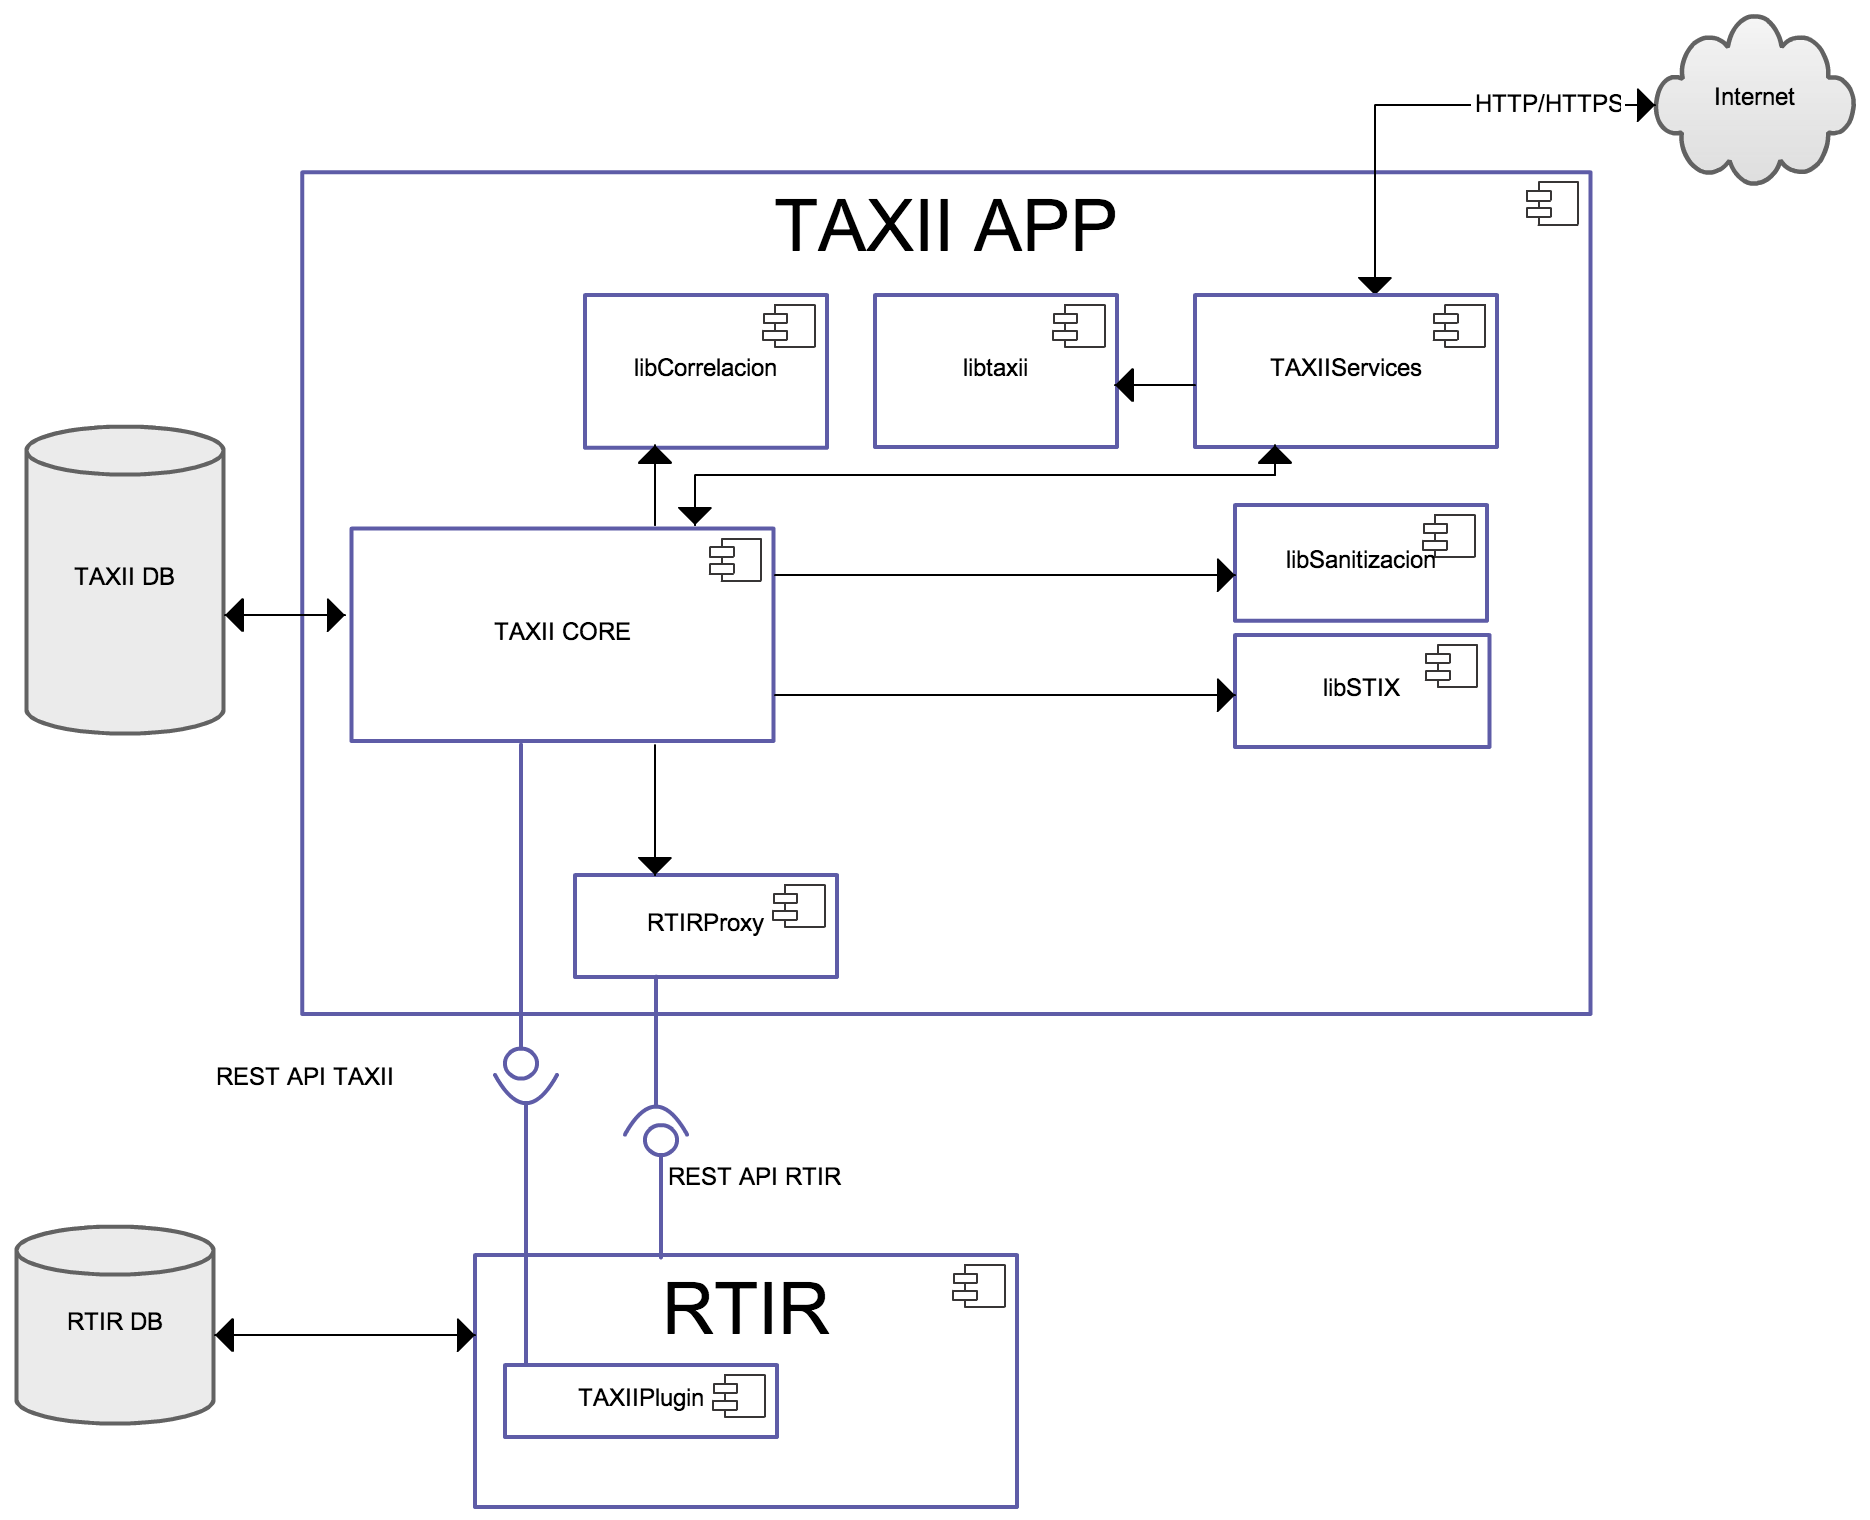
\includegraphics[width=5.7638in,height=4.6846in]{Diseno21-img/Diseno21-img003.png} 
		\caption{Arquitecture del sistema}	
		\label{fig.arquitecturasistema}
	\end{figure}
	\bigskip
	
	
	\section[Aspectos generales de las componentes del sistema]{\foreignlanguage{spanish}{Aspectos generales de las
			componentes del sistema}}
	
	

	\foreignlanguage{spanish}{En la figura \ref{fig.arquitecturasistema} se pueden ver dos bases de datos: TAXII DB y RTIR DB. A su vez se cuenta con dos
		aplicaciones: RTIR y TAXII App. RTIR es la aplicación para manejo de incidentes desarrollada por la empresa
		Bestpractial [BP] y elegida para el desarrollo de este proyecto. TAXII App es una aplicación nueva que será
		desarrollada durante el proyecto y se encarga de representar la información de forma estructurada e intercambiar dicha
		información de seguridad.}
    \bigskip
	
	\foreignlanguage{spanish}{La aplicación RTIR recibe datos ingresados por un analista y los transmite a la aplicación
		TAXII App. Para realizar dicha transmisión es necesario extender RTIR para consumir una API REST publicada por el
		cliente TAXII. La aplicación RTIR también puede recibir de la aplicación TAXII App información, la cual puede
		estar relacionada a tickets existentes y contener soluciones a problemas, identificación de atacantes, etc.}
	
	
	\bigskip
	
	\foreignlanguage{spanish}{La aplicación TAXII recibe datos de RTIR así como también de organizaciones socias, en un
		futuro se podría dar la posibilidad de que la aplicación TAXII recibiera datos de sensores que se encuentren en la red
		de la organización. Luego de que los datos son recibidos y almacenados se correlacionan con los ya existentes. De la
		correlación se pueden obtener soluciones a problemas encontrados, información sobre ataques realizados, identificación
		de atacantes, etc. En caso de que exista información de utilidad se pueden ingresar notas a tickets o relacionar
		tickets existentes en el RTIR.}
		\bigskip
	\foreignlanguage{spanish}{También se podría compartir información con otras organizaciones para colaborar en la lucha
		contra amenazas. Para realizar dicho intercambio se representa la información utilizando STIX y luego se intercambia
		utilizando TAXII. Se utilizan librerías provistas por MITRE para realizar la representación y el intercambio de la
		información.}
	
	
	\bigskip
	
	\foreignlanguage{spanish}{La aplicación TAXII App es independiente de la aplicación RTIR, siendo posible reemplazar esta
		última por otra herramienta con funcionalidades similares. Es deseado que la herramienta que pueda reemplazar a RTIR
		pueda ser extendida de forma de invocar a las funcionalidades desarrolladas en TAXII App y cuente con un método por el
		cual la TAXII App pueda utilizar la funcionalidades de la herramienta que sustituya a RTIR.}
	
	\subsection[RTIR]{\foreignlanguage{spanish}{RTIR}}
	\foreignlanguage{spanish}{Esta componente presenta las funcionalidades originales de la herramienta RTIR con un agregado
		específico implementado para este proyecto. RTIR es la componente de la aplicación encargada de realizar el manejo de
		los incidentes. Se agrega una extensión que permite invocar una API REST en la aplicación TAXII. \ }
	\bigskip
	
	\foreignlanguage{spanish}{La base de datos de la aplicación es RTIR DB y es únicamente utilizada por la componente RTIR,
		no hay acceso desde ningún otro componente a ella. Además es importante destacar que la base de datos de RTIR no se
		modifica de ningún modo.}
	
	
	\bigskip
	
	\subsection[TAXII App\ \ \ \ \ \ \ \ ]{\foreignlanguage{spanish}{TAXII App\ \ \ \ \ \ \ \ }}
	
	\bigskip
	
	\foreignlanguage{spanish}{La segunda componente presente es TAXII App, está compuesta por otros componentes
		implementados durante el proyecto así como por librerías provistas por MITRE. Los componentes provistos por MITRE son
		libTAXII y libSTIX, a estos no se le realizaran cambios debido a que cuentan con las funcionalidades necesarias para
		llevar a cabo el proyecto. En el caso de libSTIX permite representar la información recibida por medio del lenguaje
		STIX, por otro lado libTAXII permite la creación de mensajes TAXII para que estos sean intercambiados. El componente
		TAXII App utiliza los componentes TAXIICore, RTIRProxy y TAXIIServices, estos son implementados durante el transcurso
		del proyecto. }
	
	\subsection[libTAXII]{\foreignlanguage{spanish}{libTAXII}}
	\foreignlanguage{spanish}{Es una librería que provee una representación de objetos de los mensajes TAXII, cuenta además
		con una serie de métodos para el manejo de dichos mensajes. Provee clientes para http y https. La librería se utiliza
		para generar los mensajes y dispone métodos para transformarlos a xml, estos xml son utilizados en los intercambios
		entre cliente y servidor.}
	
	\subsection[libSTIX]{\foreignlanguage{spanish}{libSTIX}}
	\foreignlanguage{spanish}{libSTIX es una librería provista por MITRE para parsear, manipular y generar contenido STIX.}
	
	\subsection[RTIRProxy]{\foreignlanguage{spanish}{RTIRProxy}}
	\foreignlanguage{spanish}{RTIRProxy es la componente de TAXII App encargada de integrarse con RTIR, para ello consume la
		API REST provista por RTIR para el manejo de tickets. Por ser una API REST la comunicación está encapsulada en el
		protocolo http. Ésta componente busca que se tenga independencia de RTIR permitiendo el uso de otro sistema en su
		lugar.}\foreignlanguage{spanish}{\ Lo que se logra es que si otro sistema tiene una API
		o un método de integración distinto al de RTIR se re implemente esta componente. La única premisa que se debe cumplir
		es que la interfaz con la cual se comunique TAXIICore se mantenga. Dentro de dichos tipos de integración podría
		encontrarse otra API REST o web services con SOAP. }
	
	\subsection[TAXIICore]{\foreignlanguage{spanish}{TAXIICore}}
	Es necesario que este componente tenga una interfaz de web services REST para realizar la
		comunicación con el RTIR. En dicha interfaz se deben dar operaciones para realizar el alta de información, obtener
		información de servicios publicados por contrapartes, enviar y recibir información de seguridad entre contrapartes.\\
		\bigskip

	Además debe proveer una interfaz para que la componente TAXIIServices envíe la información
		recibida en la aplicación TAXII, en dicha interfaz se deben recibir tanto paquetes STIX así como información adicional
		utilizada por el protocolo TAXII. \\
	\bigskip	
	\foreignlanguage{spanish}{La información tomada de la base de datos es enviada en forma de objetos STIX junto a las
		políticas definidas por los administradores para que sea sanitizada. Luego de que la información es sanitizada es
		enviada a TAXIIServices para que sea compartida con las organizaciones socias.}
	
	\subsection[libSanitizacion]{\foreignlanguage{spanish}{libSanitizacion}}
	Esta es la componente encargada de realizar la sanitización de la información que se desea
		intercambiar entre los sistemas. Para realizar dicha sanitización se podrían utilizar librerías ya existentes o implementar una
		propia. La componente se alimenta de políticas definidas por los administradores para realizar la
		sanitización.
	
	\subsection[libCorrelacion]{\foreignlanguage{spanish}{libCorrelacion}}
	\foreignlanguage{spanish}{Es la componente encargada de la correlación de los datos del sistema, dicha correlación se
		realiza por medio de políticas ingresadas por los administradores del sistema. La componente ayuda a agrupar datos que
		tengan características similares lo que facilita el trabajo de los analistas y da más valor a la información recibida.
		Se pueden utilizar distintos métodos para realizar las correlaciones y de ahí se desprende la necesidad de que sea un
		componente separado del Core del sistema. Los datos correlacionados son los almacenados en TAXII DB.}
	
	\subsection[TAXIIServices]{\foreignlanguage{spanish}{TAXIIServices}}
	\foreignlanguage{spanish}{Esta componente es una implementación de los servicios TAXII como se especifica en [M13] \ y
		\ [M14]. }
	
	\foreignlanguage{spanish}{TAXIIServices provee los siguientes servicios:}
	
	\begin{itemize}
		\item \foreignlanguage{spanish}{\underline{Inbox}: Por medio de este servicio el sistema acepta mensajes enviados por otro cliente
			TAXII en intercambios iniciados por este. }
		\item \foreignlanguage{spanish}{\underline{Poll}: Este servicio es el que utiliza el sistema para consumir datos provenientes de un
			TAXII Data Feed en un cliente TAXII.}
		\item \foreignlanguage{spanish}{\underline{Discovery}: Es el servicio encargado de la comunicación de información referente a la
			disponibilidad y uso de los servicios TAXII en el sistema.}
	\end{itemize}
	
	\bigskip
	
	\foreignlanguage{spanish}{Utiliza la componente libTAXII para crear mensajes TAXII y de esa forma realizar el
		intercambio de documentos STIX recibidos de libSanitizacion. Los mensajes que son recibidos de otros socios son pasados
		a la componente TAXIICore para que sea almacenada y luego correlacionada con datos existentes. }
	
	
	\bigskip
	
	\section[Comunicación entre los componentes]{\foreignlanguage{spanish}{Comunicación entre los componentes}}
	
	\bigskip
	
	\foreignlanguage{spanish}{En la comunicación entre RTIR y la aplicación TAXII se utiliza REST (\textit{Representational State
		Transfer}), en este tipo de servicio web se trata de emular \ el protocolo http o algún protocolo similar usando la
		restricción de proveer una interfaz a un conjunto conocido de operaciones estándar (GET, PUT, etc). Se utiliza este
		tipo de servicio web debido a que RTIR provee una API de este tipo. }
	
	
	\bigskip
	
	\foreignlanguage{spanish}{El intercambio entre las distintas organizaciones se realiza por medio de HTTP/HTTPS. Esto se
		debe a que hasta el momento MITRE solo ha especificado el intercambio por medio de dicho protocolo. Se podrían utilizar
		otros protocolos para realizar el intercambio pero sería necesario que MITRE definiera las especificaciones para su
		uso, un ejemplo de ellos podría ser SOAP.}
	
	
	\bigskip
	
	\section[Modelo de datos]{\foreignlanguage{spanish}{Modelo de datos}}
	\foreignlanguage{spanish}{El modelo de datos diseñado se adapta a las necesidades de TAXII, dichas necesidades están
		definidas en \ [M15], además se agrega una tabla para realizar el mapeo entre los elementos de RTIR y los elementos
		TAXII intercambiados. En la figura \ref{fig.diagramadedatos} se ve el modelo de datos \ y a continuación se explica cada una de sus
		componentes.}
	
	\begin{figure}[ht!]
	\centering
	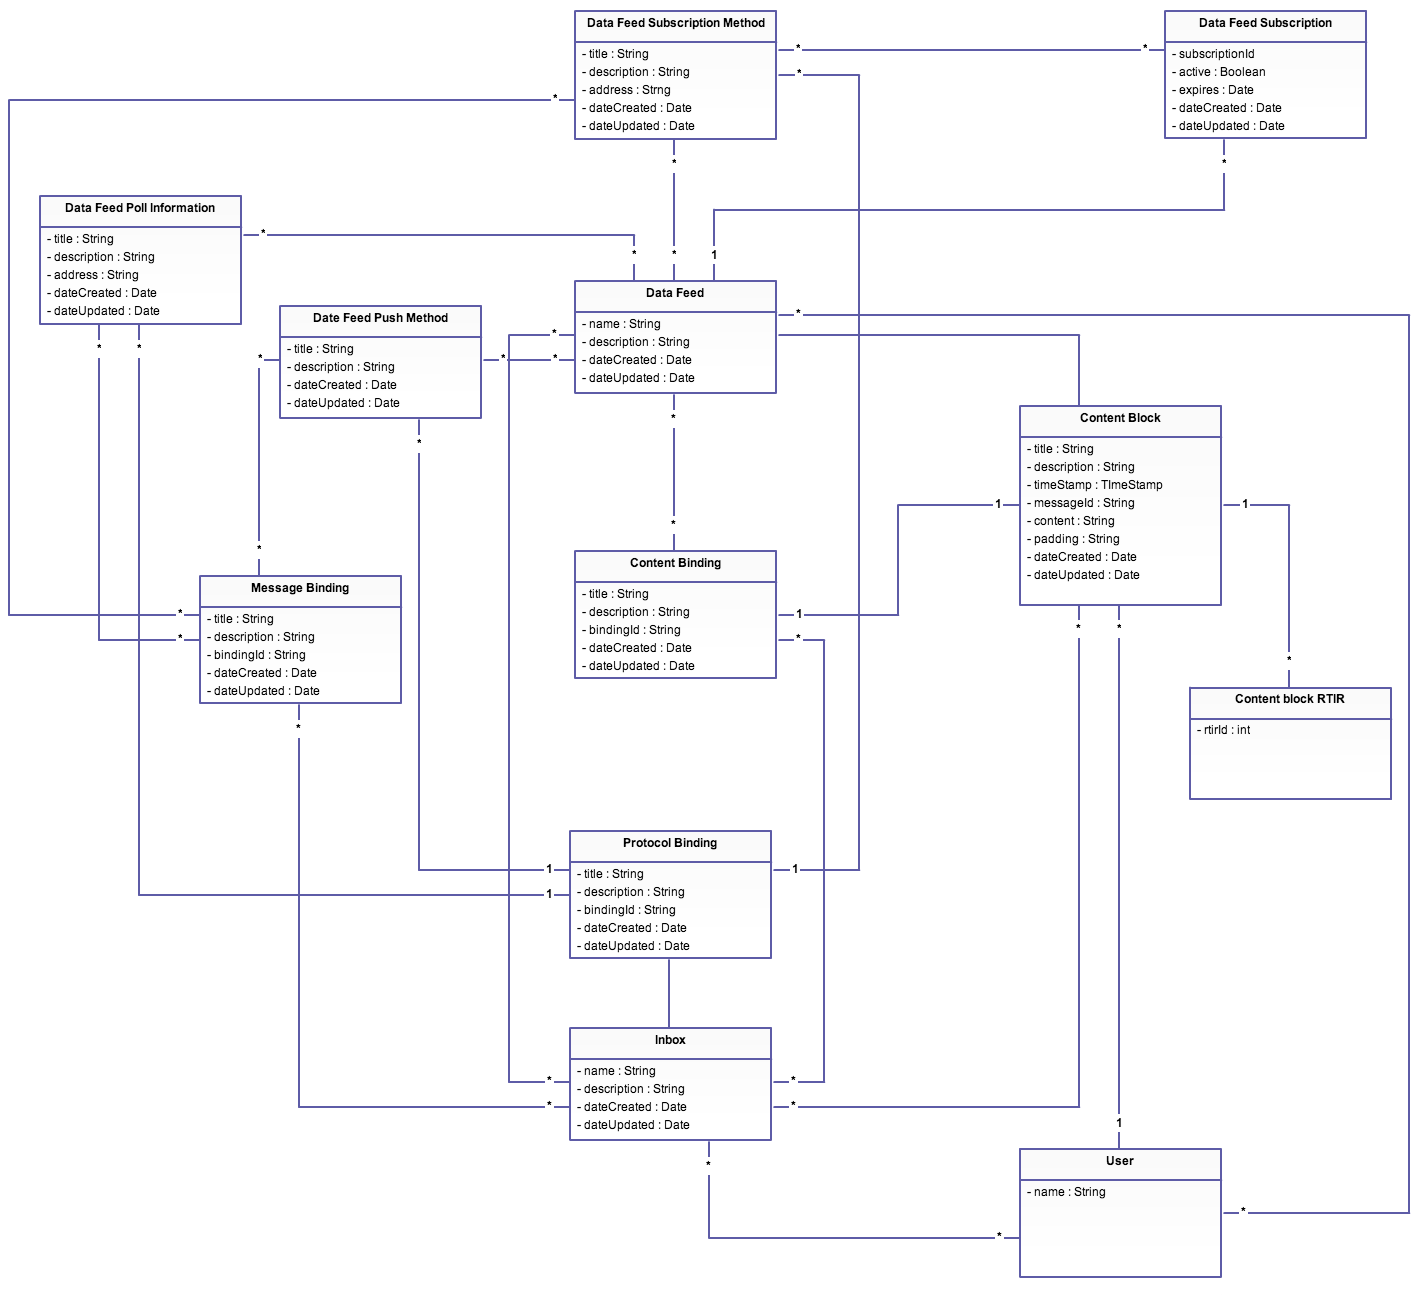
\includegraphics[width=5.7638in,height=5.3126in]{Diseno21-img/Diseno21-img004.png} 
	\caption{Diagrama de datos}
	\label{fig.diagramadedatos}
	\end{figure}
	\bigskip
	
	
	\begin{itemize}
		\item \foreignlanguage{spanish}{\underline{Protocol Binding}: Es un elemento utilizado para establecer el protocolo de intercambio
			soportado por una implementación de TAXII.}
		\item \foreignlanguage{spanish}{\underline{Content Binding}: Es utilizado para establecer el tipo de contenido soportado para un
			cierto intercambio realizado con TAXII, por ejemplo:
		}\foreignlanguage{spanish}{\textit{Poll}}\foreignlanguage{spanish}{,
	}\foreignlanguage{spanish}{\textit{Inbox}}\foreignlanguage{spanish}{, etc.}
	\item \foreignlanguage{spanish}{\underline{Message Binding}: Es utilizado para establecer el tipo de sintaxis para un intercambio
		realizado con TAXII.}
	\item \foreignlanguage{spanish}{\underline{Data Feed Push Method}: Es utilizado para establecer los protocolos que pueden ser
		utilizados para enviar contenido por medio de una subscripción. Esto se utiliza en un mensaje de tipo
	}\foreignlanguage{spanish}{\textit{Feed Information Response}}\foreignlanguage{spanish}{. Es definido en [M14].}
	\item \foreignlanguage{spanish}{\underline{Data Feed Poll Information}: Tiene la finalidad de establecer los protocolos soportados y
		las direcciones de una fuente de información (}\foreignlanguage{spanish}{\textit{Data
			Feeds}}\foreignlanguage{spanish}{). Es utilizado en los mensajes de }\foreignlanguage{spanish}{\textit{Feed Information
			Response}}\foreignlanguage{spanish}{ como se define en [M14].}
	\item \foreignlanguage{spanish}{\underline{Data Feed Subscription Method}: Es utilizado para identificar el protocolo y la dirección
		de un servicio de }\foreignlanguage{spanish}{\textit{Feed Managment}}\foreignlanguage{spanish}{ que pueda procesar las
		subscripciones a fuentes de información TAXII.}
	\item \foreignlanguage{spanish}{\underline{Content Block}: Representa el contenido de los mensajes
	}\foreignlanguage{spanish}{\textit{Poll Response }}\foreignlanguage{spanish}{o }\foreignlanguage{spanish}{\textit{Inbox
		Messages}}\foreignlanguage{spanish}{. Es necesario señalar que el campo
}\foreignlanguage{spanish}{\textit{content}}\foreignlanguage{spanish}{ representa un mensaje STIX. Dicho mensaje
representa la información de seguridad estructurada, la cual fue representada utilizando el lenguaje STIX.}
\item \foreignlanguage{spanish}{\underline{Data Feed}: Representa una fuente de información TAXII, los usuarios se suscriben a
	dichas fuentes de información para recibir datos que sean de su interés. }
\item \foreignlanguage{spanish}{\underline{Data Feed Subscription}: Representa una subscripción a fuentes de datos TAXII.}
\item \foreignlanguage{spanish}{\underline{Inbox}: Representa un }\foreignlanguage{spanish}{\textit{inbox
	}}\foreignlanguage{spanish}{TAXII, estos son el mecanismo por el cual los consumidores reciben información de otros
	clientes TAXII que nos envían información. La representación permite que un
}\foreignlanguage{spanish}{\textit{inbox}}\foreignlanguage{spanish}{ este asociado a ningún o muchas fuentes de datos.
}
\item \foreignlanguage{spanish}{\underline{Content Block RTIR}: Representa el nexo entre los contenidos TAXII y los tickets
	existentes en RTIR.}
\end{itemize}
\chapter{Implementación}
\label{capitulo5}
\section{Aspectos Generales}
En esta sección se presentan las herramientas y metodologías elegidas para realizar la implementación de la herramienta.

\subsection{Entorno de desarrollo}
El entorno desarrollado durante la implementación del sistema y desarrollo del caso de estudio consta de:

\begin{itemize}
	\item Sistemas operativos: Mac OS 10.9.3 (Maverick) y Linux Mint 15
	\item Sistemas operativos utilizados en el testeo y caso de estudio: Linux Mint 15
	\item Lenguajes de desarrollo: Perl y Python (web framework Django)
	\item Entorno de desarrollo: vim\footnote{Vim es un editor de texto que está diseñado para usarse tanto desde una interfaz de línea de comandos o como una aplicación independiente en una interfaz gráfica de usuario.}  con plugins provistos por spf13\footnote{http://vim.spf13.com/ centraliza un conjunto de plugins para vim.}
	\item Base de datos: Mysql versión 14.14 distribución 5.5.34
	\item Sistema de versionado: git
	\item Servidor web: apache2
	\item Versión de RT: RT4
	\item Testeo de APIs Rest: Postman\footnote{Es una herramienta de chrome utilizada para probar, desarrollar y documentar APIs.}
	
\end{itemize}

\subsection{Metodología}

Se utilizó el framework web Django por permitir desarrollar aplicaciones web de forma rápida y con la escritura de poco código. Además busca automatizar parte del desarrollo al basarse en el principio DRY (\textit{Don’t Repeat Yourself}). Presenta la ventaja de utilizar el patrón de arquitectura MVC (\textit{Model View Controller}). La ventaja de utilizar este patrón es que divide la aplicación en tres partes interconectadas y da una base inicial con la cual desarrollar el trabajo. A su vez, utilizar un patrón MVC presenta la ventaja de que se tiene experiencia desarrollando aplicaciones utilizando dicho patrón lo cual facilita el trabajo.
La existencia de librerías implementadas en python para trabajar con STIX y TAXII influyo fuertemente en la decisión de utilizar Django. Otra de las razones fue la existencia de una implementación de referencia con la cual se puede testear el desarrollo realizado.\\
	\bigskip
Además de utilizar Django se utilizó el lenguaje de programación PERL para el desarrollo de un plugin para la herramienta RT.\\

	\bigskip
La metodología utilizada fue la de un desarrollo incremental, esto permitió realizar una validación de la arquitectura propuesta. Luego de realizar dicha validación se siguió implementando la herramienta propuesta.

\subsection{Librerias utilizadas}
Durante el transcurso de la implementación se utilizaron distintas librerías Perl y Python para el desarrollo de la herramienta.

\subsubsection{Django Rest Framework}
Django Rest Framework \cite{rest_framework} es una librería para Django que hace simple el construir APIs REST de forma sencilla y rápida. La librería se utilizó para implementar la API REST que se consume desde el plugin RT-TAXII, dicho plugin se explicará mas adelante.

\subsubsection{LWP}
LWP se refiere a LibWww-Perl \cite{lwp} y es un conjunto de módulos Perl que proveen una API simple para desarrollar clientes web y desarrollar servidores http. En particular se utilizó el módulo LWP::UserAgent que permite realizar con facilidad pedidos web.
Con esta librería se realizan los pedidos que se hacen a la componente  libTAXII.

\subsubsection{libTAXII}
libTAXII \cite{libtaxii} es una librería Python para manejar mensajes TAXII e invocar servicios TAXII. Uno de sus objetivos es ser fiel a las especificaciones de TAXII y a las buenas prácticas de Python.
La librería provee:

\begin{enumerate}
	\item
	Una representación de objetos de los mensajes TAXII.
	\item
	Permite transformar XML en objetos Python y viceversa.
	\item
	Un cliente HTTP/HTTPS TAXII.
\end{enumerate}

Esas tres características se utilizaron durante el desarrollo de la herramienta. Debido a que primero se crea un objeto Python que representa el mensaje TAXII, dicho objeto es transformado a XML para ser enviado por el cliente TAXII, la respuesta al mensaje enviado también es un objeto XML, dicho XML es transformado a un objeto Python para ser procesado.
A su vez cuando se recibe un XML, este se transforma a un objeto Python para ser procesado, luego del procesamiento se devuelve una respuesta XML por medio del cliente HTTP/HTTPS.

\subsubsection{pythonStix}
PythonStix \cite{pythonstixgit} es una librería Python que provee una API para parsear, manipular y consumir contenido STIX. Los desarrolladores pueden utilizar la API para desarrollar aplicaciones que crean, consumen, traducen o procesen contenido STIX.
Se utilizo en taxiiApp para crear paquetes STIX a partir de un cyber observable que ingrese el usuario en RTIR. Además durante los intercambios se obtiene información de los paquetes STIX para lo cual es necesario parsear la información del paquete STIX. 


\subsubsection{YETI}
YETI \cite{yeti} es una prueba de concepto de TAXII creado para ayudar a los desarrolladores a implementar y testear sus propias aplicaciones TAXII. A su vez ayuda a aprender más sobre el funcionamiento de TAXII.
Fue utilizada en etapas tempranas del proyecto como referencia y para testear el desarrollo realizado. De esta forma mientras se avanzó en el desarrollo se pudo validar de forma adecuada que se respetara adecuadamente la especificación de TAXII.

\subsection{Módulos desarrollados}
A continuación se describen lo módulos implementados para el funcionamiento de la herramienta, así como las consideraciones necesarias para extender la herramienta con nuevas funcionalidades.

\subsubsection{RT-TAXII}
Se desarrolló un plugin para RTIR que es el encargado de consumir la API rest provista por TAXIIApp y que extiende la interfaz web de RTIR para presentarle al usuario los formularios necesarios para que interactúe con el sistema.
Se incluyó en el menú de RTIR una nueva sección en la que se especifican las distintas acciones que se pueden realizar referentes a TAXII.
Cada una de estas acciones invoca a un script desarrollado en PERL que presenta el formulario al usuario.
Luego de que el usuario ingresa la información deseada y realiza el envío de la información. El sistema invoca a la API Rest provista por TAXII App.
Es necesario que se configure la dirección del host en la que se encuentra ejecutando TAXIIApp.
La estructura de directorios de RT-TAXII es la que se muestra en la figura \ref{fig.rt_taxii}.\\

\begin{figure}[H]
	\centering
	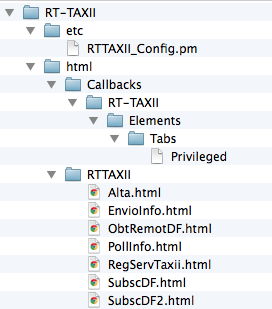
\includegraphics{imagenes/RT-TAXII.png}
	\caption{Estructura de directorios de plugin RT-TAXII}
	\label{fig.rt_taxii}
\end{figure}
	\bigskip
El archivo RTTAXII\_Config.pm es utilizado para guardar las configuraciones del plugin. Dentro de dichas configuraciones se encuentran parámetros necesarios para el funcionamiento del sistema.
En el archivo Privileged se realiza la configuración del menú que contiene las funcionalidades del sistema.
Los archivos incluidos en el directorio RTTAXII son los encargados de presentar los formularios y realizar la lógica correspondiente a las llamadas a TAXIIApp. Dichos archivos están implementados en PERL y contienen HTML para realizar la presentación al usuario.\\

Para extender la herramienta con nuevas funcionalidades es necesario crear un nuevo script PERL en el directorio RTTAXII. Dicho script debe implementar las funcionalidades que se deseen. Como RT está desarrollado en PERL se cuenta con todos los módulos disponibles de PERL.

\subsubsection{TAXIIApp}
A continuación se describirán los componentes implementados y como estos interactúan con las librerías utilizadas.
También se mencionarán las consideraciones que se deben tener para expandir la herramienta.
En la figura \ref{fig.taxii_app} se ven los distintos módulos implementados durante el proyecto. 

\begin{figure}[H]
	\centering
	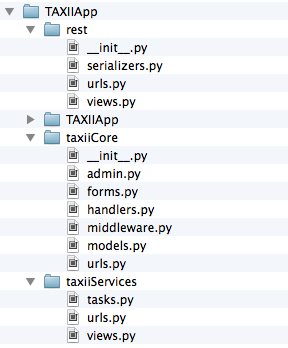
\includegraphics{imagenes/TAXIIApp.png}
	\caption{Aplicación TAXII implementada junto con sus módulos}
	\label{fig.taxii_app}
\end{figure}
\bigskip
\paragraph{TAXIICore}\ \\
TAXII Core es la componente encargada del procesamiento de la información, es invocada por la API Rest y por TAXII Services y actúa dependiendo de la información recibida. Además es la encargada de la comunicación con la base de datos por medio del modelo de datos desarrollado. A su vez se tuvo consideración durante el desarrollo que este componente sería el encargado de dialogar con los módulos de sanitización y correlación de información. 
En el anexo \ref{anexo} se pueden ver las entidades creadas para modelar la base de datos así como los métodos implementados para enviar y recibir información del resto de las componentes.

\paragraph{TAXIIServices}\ \\
Este módulo es el encargado de la comunicación con otra organización por medio del protocolo TAXII. Se desarrollaron  los distintos métodos necesarios para implementar los servicios TAXII exceptuando el discovery service.
Se utiliza libTAXII para crear los mensajes a intercambiar y para realizar la invocación a los servicios de otras organizaciones.
Los mensajes luego de recibidos son pasados a TAXIICore para su procesamiento.
En caso de que se crearan nuevos servicios o que se quisiera implementar por ejemplo el discovery service esto se realizaría en este módulo.
En el anexo \ref{anexo} se pueden ver las firmas de los servicios implementados.

\paragraph{REST API}\ \\
La API Rest desarrollada provee las funcionalidades necesarias para que RT-TAXII interactúe con TAXII App. Dentro de dichas interacciones se permite el manejo de cualquiera de los elementos del modelo en TAXIICore. Además se crearon métodos específicos para el uso de TAXII. Se permite el envío y poll de información, obtención de data feeds así como la subscripción a estos.\\

Para la implementación se utilizo la librería auxiliar \textit{Django Rest framework} que simplifica el desarrollo de la API.
Si bien se implementaron todos los elementos necesarios para realizar la interacción con la base de datos, si existiera un cambio en esta (i.e: se crea una nueva entidad) sería necesario extender esta API para poder realizar la interacción entre los sistemas. A su vez si se crea un nuevo servicio TAXII y se desea proveer una interfaz en RTIR para que los usuarios interactúen con esta sería necesario agregar los métodos necesarios en esta API.
En el anexo \ref{anexo} se puede ver la firma de la API desarrollada.


\subsection{Alcance}

Durante el proyecto se pusó foco en el intercambio de información de seguridad de forma estructurada, por ello se recortó el alcance respecto eliminando algunas funcionalidades que se mencionaron durante el analisis del problema. Dichas funcionalidades quedan planteadas como trabajo futuro para el proyecto.

El no desarrollo de un modulo de correlación se debió al tiempo que llevaria realizar una investigación en profundiad enfocada en correlación de investigación de seguridad. Al no poseer un módulo de correlación de información perdió sentido el tener un caso de uso para realizar el alta, baja y modificación de políticas de correlación.

Tampoco se implementó el modulo de sanitización de información, debido a que también hubiera llevado mucho tiempo investigar e implementar un modulo de sanitización de información de seguridad. Como en el caso del modulo de correlación también perdieron sentido los casos de uso de alta, baja y modificación de politicas de sanitización.

No se implementó el discovery service del protocolo TAXII debido a que ingresando manualmente los servicios TAXII se obtiene el mismo resultado. En caso de que se implementara seria necesario agregar un caso de uso para dar de alta una nueva URL para organización. Es necesario recordar que no es necesario implementar todos los servicios TAXII especificados.

No se integró el sistema de gestión de usuarios que tiene Django, esto es necesario para tener un seguimiento de los usuarios u organizaciones con las que se intercambia información.

\chapter{Caso de estudio}

\chapter{Conclusiones y trabajo futuro}
\label{capitulo7}

En este capítulo se presentan las principales conclusiones y dificultades más relevantes del proyecto. Por último, se proponen posibles líneas de trabajo a futuro.

\section{Trabajo Futuro}
Durante el transcurso del proyecto se identificaron distintas líneas de trabajo futuro sobre las cuales se puede trabajar para mejorar la herramienta. A continuación delineamos algunos de los trabajos que se podrían seguir realizando en el marco de este proyecto.
\bigskip

Como es posible que se intercambien grandes volúmenes de datos entre organizaciones, es necesario que se diseñe e implemente un método para correlacionar la información intercambiada, de esta forma se agrupan los datos, facilitando de esta forma el trabajo de los analistas. Con dicha información correlacionada se pueden presentar reportes a los analistas resumiendo el contenido existente en el sistema. Durante el diseño y análisis de la herramienta se tuvo en consideración dicha funcionalidad pero no se implementó y no hubo una investigación profunda referente a esto, por lo cual se deja para un trabajo a futuro. 
De la misma forma se consideró durante el diseño y análisis la sanitización de la información pero tampoco se implementó en el prototipo dicha funcionalidad quedando para un trabajo a futuro.  Dicha funcionalidad permite filtrar datos sensibles que podrían comprometer la imagen o la integridad de las organizaciones.
\bigskip

Respecto a la implementación realizada, queda planteado realizar una mejor interacción entre RTIR y el \textit{plugin} de forma de extender las funcionalidades ya existentes en RTIR así como agregar algunas nuevas. Entre dichas mejoras se encuentra crear los incidentes y relacionarlos con los cyber observables existentes en TAXII App. Además permitir agregar nuevos cyber observables a incidentes ya existentes. Esto, junto con una interfaz más amigable facilitaría  el trabajo de los analistas.
\bigskip

Otro de los puntos a mejorar en la implementación del cliente TAXII es el seguimiento de los usuarios u organizaciones con las que se intercambia la información de seguridad y filtrar a que datos pueden acceder los distintos usuarios. De esta forma se podría realizar un modelo RBAC para el acceso a la información.
\bigskip

\section{Conclusiones}

En los últimos años se ha visto un incremento en la cantidad de equipos conectados a las redes de las organizaciones, a su vez han aumentado los usuarios malintencionados. Estos cuentan cada vez con mejores herramientas y procedimientos mas sofisticados con los cuales realizar ataques. Debido a esto es necesario que las estrategias de defensa se adapten a los nuevos actores y ataques. Para responder a esto, las organizaciones han recurrido al intercambio de información de amenazas con la finalidad de identificar de mejor forma las actividades de sus adversarios con la finalidad de obtener los mejores resultados posibles de sus defensas.\\
\bigskip
Durante el estado de arte se vieron diferentes problemas que dificultan el intercambio de información de seguridad entre las organizaciones. Estos van desde problemas que son estrictamente técnicos a otros que son de índole política. En este punto se decidió centrarse en los problemas que son estrictamente técnicos y se identificaron cuales son los enfoques utilizados en la actualidad para el intercambio de información. Se vio que las  herramientas que son utilizadas actualmente se enfocan en una parte del problema y que en muchos casos el intercambio de información es realizado entre humanos.  \\
\bigskip
Durante el transcurso del proyecto se vio el fuerte interés que existe en las organizaciones por llegar a un consenso respecto a estándares utilizados en el intercambio de información de seguridad.  En particular resultaron llamativas las iniciativas de MITRE que cuentan con el apoyo tanto de organizaciones provenientes del sector publico así como del sector privado y las cuales provienen de distintos sectores de la industria.\\   
\bigskip
La existencia de estos estándares es fundamental para lograr un buen nivel de automatización. Si bien se puede automatizar sin que un estándar sea apoyado por la comunidad, el esfuerzo que se debe realizar para poder integrar conocimientos es muy grande. Esta integración de conocimientos es clave para fomentar el avance de las herramientas, técnicas y metodologías, que permitan contrarrestar el impacto de los ataques automatizados.\\
\bigskip
El esfuerzo encabezado por MITRE busca desarrollar un conjunto de estándares referentes a la caracterización e intercambio de información de seguridad. Intenta proveer lenguajes que permitan facilitar la comunicación de la información de seguridad de forma precisa. Algunos de los lenguajes son CYBOX, STIX, CAPEC, entre otros. Junto con estos esfuerzos utilizados para la representación de la información se encuentra TAXII. TAXII también es un esfuerzo de MITRE que busca estandarizar el intercambio confiable y automático de información. TAXII tiene como finalidad ayudar en el intercambio de información entre las organizaciones que lo deseen utilizando relaciones y sistemas existentes. No se busca que TAXII defina métodos de confianza entre las organizaciones o cualquier aspecto no técnico del intercambio de información de seguridad.\\
\bigskip
También durante el estudio del arte se estudio RTIR y algunas otras herramientas que cuentan con características similares. RTIR ha sido una herramienta desarrollada junto con CSIRTs para el manejo de incidentes de seguridad. Permitiendo que se agregue información asociada a estos.\\
\bigskip
El estudio del arte no fue una tarea sencilla debido a la amplitud de la temática tratada y por la cantidad de información encontrada. Se tuvo a disposición mucha información de múltiples fuentes. Se vieron temas referentes a la correlación de la información así como de la sanitización de ésta y como estas dos tareas afectan fuertemente el trabajo y la reputación de las organizaciones. A su vez se dio mucha importancia a la representación de información de forma estructurada.\\
\bigskip
Luego de terminado el estado del arte se realizó el análisis evaluando los distintos problemas identificados durante el estado del arte. Se identificaron algunos problemas que eran de interés para el proyecto. De dichos problemas se identificaron requerimientos que son deseables en una herramienta que intercambia información de seguridad.\\
\bigskip
Se realizó el diseño de la herramienta utilizando STIX, TAXII y RTIR y centrándose en el intercambio y la representación de información de forma estructurada. El diseño realizado buscó solucionar los requerimientos planteados en el análisis. De ésta forma, se tuvieron en cuenta durante el diseño problemáticas referentes a la correlación y sanitización de la información que se dejaron planteados como trabajos futuros. La arquitectura planteada busca ser extensible y modular, permitiendo la interacción con herramientas de gestión de incidentes distintas a RTIR y la extensión de las funcionalidades ya existentes en el sistema.\\
\bigskip
Luego de realizado el diseño se realizó un prototipo de la herramienta propuesta. Esta intercambia información utilizando el protocolo TAXII y representando la información por medio de STIX. El manejo de la información se realiza desde RTIR dando de alta los datos necesarios para realizar el intercambio. Es necesario destacar la dificultad en la implementación de un \textit{plugin} para RTIR que no fue una tarea sencilla y que se realizó por medio de ingeniería reversa de un \textit{plugin} ya existente. Además se implementó un cliente que implementa el protocolo TAXII para realizar el intercambió que además cuenta con una API REST que puede consumir el \textit{plugin} RTIR.\\
\bigskip
Finalmente se ideó un caso de estudio en el que se intercambian cyber observables entre dos organizaciones por medio del protocolo TAXII utilizando los distintos servicios provistos en su especificación.

\nocite{*}
\bibliographystyle{plain}
\bibliography{biblio}
% *************** Back matter ***************

% ***************************************************************************
% You can disable here list of symbols, list of figures, and list of tables.
% You can also disable index generation.
% ***************************************************************************



\normalfont
\clearpage
%\input{symbols.tex}

\clearpage
\listoffigures

\footnotesize

% *************** End of back matter ***************

%\section{Estado del Arte}
%\label{anexo.estadodelarte}

%\subsection{Gestión de incidentes}
%\label{anexo.gestiondeincidentes}
%\subsubsection{Herramientas}
%\label{anexo.herramientas}
%\subsubsection{Que es RTIR}
RTIR es un sistema de manejo de incidentes diseñado para ser utilizado por los 
equipos de seguridad de sistemas. A sido creado en conjunto con equipos de CERT 
y CSIRT para manejar el creciente número de incidentes reportados.
Presenta la ventaja de ser opensource, contener una API completa y una comunidad 
de usuarios grande y experta. Además es simple de integrar con otras 
herramientas existentes. Está implementado por medio de módulos PERL y las 
herramientas que provee RT. Se puede pensar en RTIR como una extensión de RT 
para ser utilizada por CERT's y CSIRT's.

Existen algunas alternativas a RTIR como lo son AIRT (Application for Incident Response Teams) 
cuya última versión data de Julio de 2009. AIRT es una aplicación web 
desarrollada para los equipos de respuesta a incidentes. Busca proveer facilidad 
ante los reportes de incidentes de seguridad así como un seguimiento simple de 
estos. Este sistema no cuenta con una comunidad comparable a la de RTIR así como 
con documentación tan extensa como la de RTIR.

Otra de las opciones existentes es OTRS (Open Technology Real Services), así 
como los anteriores también es open soruce. Presenta las ventajas de tener una 
comunidad más numerosa que AIRT y que el código esta siendo desarrollado continuamente. 
Así como RTIR esta desarrollado por medio de Perl y permite conectarse a varias 
bases de datos. Presenta documentación extensa para implementadores.

%\subsection{Representación}
%\label{anexo.representacion}
%\subsubsection{Modelos de datos}
%\label{anexo.modelodedatos}
%Aca se podria poner algo de openIOC

%\subsubsection{IDMEF}

Intrusion Detection Message Exchange Format (IDMEF) fue especificado como un 
protocolo experimental que no especifica ningún estándar. El propósito de 
IDMEF es definir formatos de datos y procedimientos de intercambio para 
compartir información de interés con sistemas de detección de intrusos y 
sistemas de respuesta con los sistemas de administración que deben 
interactuar con estos. El RFC de IDMEF describe el modelo de datos para 
representar información tomada de los sistemas de intrusión. Se busca que dicho 
formato pueda ser utilizado por los Intrusion Detection Systems (IDSs) para 
reportar alertas sobre eventos que parezcan sospechosos.

Por medio de la firma digital de XML se busca proveer integridad, autenticidad de 
los mensajes y de los servicios. La responsabilidad para la integridad y 
autenticación de los mensajes es responsabilidad del protocolo de comunicación y 
no del formato de mensajes. La inclusión de firmas digitales en mensajes IDMEF 
debería ser realizada en casos en los que éstas deban ser archivadas para su uso 
posterior o cuando los mensajes IDMEF son intercambiados sobre protocolos poco 
seguros.

\paragraph{Modelo de datos de IDMEF}
El modelo de datos de IDMEF es una representación orientada a alertas enviadas a 
los administradores desde los sistemas de intrusión. El modelo de datos presenta 
varios problemas referentes a la representación de los datos:
\begin{itemize}
  \item Generalmente, la información de las alertas es heterogénea. Algunas 
  alertas son definidas con poca información, otras proveen información más 
  detallada. Ejemplos de alertas con poca información son aquellas que solo 
  presentan datos de origen, destino, nombre u hora, estos datos pueden set 
  extendidos por alertas detalladas en las cuales se presenta información de 
  usuarios, procesos o puertos de servicios. Es necesario que el modelo de datos 
  que represente dicha información sea flexible para adaptarse a las distintas 
  necesidades. Un modelo de datos orientado a objetos es extensible por medio de 
  agregación y sub clases, de esta forma una implementación que no entienda 
  estas extensiones podrá seguir entendiendo el subconjunto de información que 
  está definido en el modelo. Estas dos formas de extender el modelo permiten 
  que se mantenga su consistencia.
  \item Los IDSs son diferentes, algunos de estos detectan ataques analizando el 
  tráfico en la red, otros utilizando los logs de sistemas operativos o 
  aplicaciones que auditan información. Las alertas generadas para un mismo 
  ataque pero por medio de diferentes herramientas, no necesariamente contienen 
  los mismos datos. El modelo de datos define clases que soportan las 
  diferencias en las fuentes de los datos. En particular, las nociones de 
  fuente y objetivo para la alerta son representadas por una combinación de 
  nodo, procesos, servicio y clases de usuario.
  \item Dependiendo del tipo de red o sistema operativo utilizado, los 
  ataques serán observados y reportados de manera diferente lo cual lleva a que 
  el modelo de datos deba adaptarse a dichas diferencias.
  \item Los instrumentos comerciales persiguen objetivos diferentes. Por varias 
  razones, estos desean entregar más o menos información sobre ciertos tipos de 
  ataques. El modelo debe permitir la flexibilidad necesaria preservando su 
  integridad.
\end{itemize}

El diseño del modelo de datos busca proveer una representación estándar de las 
alertas de manera que la información no sea ambigua y que se describa la 
relación entre alertas simples y complejas.

El objetivo de dicho modelo es proveer una representación estándar de la 
información analizada por un sistema de intrusión cuando es detectado 
un evento inusual. Estas alertas pueden ser simples o complejas 
dependiendo de las capacidades de la herramienta que las creo.

Los nuevos objetos son introducidos para referenciar contenido adicional. Esto 
es importante debido a que la tarea de clasificar y nombrar vulnerabilidades es 
difícil y sumamente subjetiva. El modelo de datos no debe ser ambiguo, por lo 
que mientras que se permite que los análisis sean más o menos precisos 
entre ellos, no se debe permitir que estos produzcan información contradictoria  
en dos alertas que describen el mismo evento. De todas formas, siempre es 
posible insertar toda la información útil de un evento en campos de extensión 
de la alerta en lugar de en los campos a los que estos pertenecen, sin embargo, 
dichas prácticas reducen la interoperabilidad y deberían ser evitadas en lo 
posible.



%\subsubsection{IODEF}

\textit{Incident Object Description Exchange Format} (IODEF) define una representación de datos que provee un framework para el 
intercambio de información entre CSIRTs, dicho tipo de información de seguridad 
es comúnmente intercambiado entre este tipo de organizaciones. IODEF provee una 
representación en XML para transportar información de incidentes entre pares en 
distintos dominios administrativos pero que tienen las responsabilidades 
operacionales de remediar o analizar y establecer advertencias en un dominio 
definido. El modelo de datos provisto por IODEF codifica la información 
referente a hosts, redes y servicios corriendo en estos sistemas; metodología 
de ataques y evidencia forense asociada; impacto de la actividad realizada y
aproximaciones a los trabajos realizados.\\

IODEF debería ser compatible con IDMEF y tener la capacidad de incluir mensajes 
IDMEF. Los actores principales en IODEF son los CSIRTs y no los IDSs como ocurre 
en IDMEF. Se puede ver a IODEF como una interfaz orientada a ser utilizada por 
personas, por ello un mensaje IODEF es parseable por una máquina y a su vez 
leíble por humanos. Los objetos IODEF tienen un tiempo de vida mayor a IDMEF, 
en éste último los mensajes son utilizados una sola vez. Los mensajes IODEF consideran 
información referente al manejo de incidentes, almacenamiento de dicha 
información o estadísticas y análisis.\\

El objetivo primordial de IODEF es mejorar las capacidades operacionales de los 
CSIRTs. La adopción por parte de la comunidad provee una habilidad mejorada para 
resolver los incidentes y transmitir información de contexto simplificando la 
colaboración e intercambio de datos.
El formato estructurado provisto por IODEF permite:
\begin{itemize}
  \item Incrementar la automatización en el procesamiento de los datos.
  \item Bajar el esfuerzo necesario para normalizar datos similares de 
  diferentes fuentes.
  \item Un formato común con el cual construir herramientas interoperables para 
  el manejo de incidentes y análisis subsecuente, específicamente cuando 
  los datos provienen de dominios distintos.
\end{itemize}

La coordinación entre CSIRTs no es un problema estrictamente técnico. La 
confianza, los procedimientos y las leyes son consideraciones que pueden impedir 
que las organizaciones intercambien información. IODEF no busca evadir dichas 
consideraciones, sin embargo, las implementaciones operacionales de IODEF deben 
considerar este contexto.

\paragraph{Modelo de datos de IODEF}\ \\

A la hora de diseñar IODEF se realizaron ciertas consideraciones de diseño:
\begin{itemize}
  \item El modelo de datos sirve como formato de transporte, lo que lleva a que 
  su representación específica no sea óptima para almacenamiento en disco, 
  ser archivado por plazos largos o procesamiento en memoria.
  \item Por medio de la implementación no se busca establecer un consenso 
  respecto a la definición de un incidente, en su lugar se trata de dar un 
  entendimiento amplio que sea lo suficientemente flexible para abarcar la 
  mayoría de las operaciones.
  \item Describir un incidente para todas las definiciones requeriría un modelo 
  de datos extremadamente complejo. Por ello, IODEF solo busca dar un marco para 
  transmitir información de incidentes comúnmente intercambiada. Se asegura un 
  mecanismo que pueda ser extendido para soportar información de la 
  organización así como técnicas para referenciar información mantenida por 
  fuera del modelo de datos.
  \item El dominio de análisis de seguridad no está totalmente estandarizado y 
  debe basarse en descripciones textuales. IODEF busca conseguir un balance 
  entre el contenido libre y el procesamiento automático de la información de 
  incidentes.
  \item IODEF es una de las representaciones que han sido estandarizadas.
   El modelo de datos de IDMEF influenció el diseño de IODEF.

\end{itemize}

El modelo de datos de IODEF no introduce problemas de seguridad. Este solo 
define una representación simple para información de incidentes. Como los datos 
codificados por IODEF pueden ser considerados sensibles por las partes que los 
intercambian se deben tomar precauciones para asegurar la confidencialidad 
durante el intercambio y el subsecuente procesamiento. El primero debe ser 
resguardado por un formato de mensaje, pero luego se deben tener consideraciones 
de seguridad en el sistema que procesa los datos, los almacena y archiva la 
documentación y la información derivada de éstos.\\

El formato de mensajes subyacente y el protocolo utilizado para intercambiar 
datos provee una garantía de confidencialidad, integridad y autenticidad. El uso 
de protocolos de seguridad estandarizados es recomendado, por ejemplo 
IODEF/RID.

\paragraph{Trabajo de MILE}\ \\

\textit{Managed Incident Lightweight Exchange} (MILE) es un grupo de trabajo del IETF que 
enfoca sus esfuerzos en dos áreas. La primera es el formato de datos y 
extensiones para representar incidentes y datos de indicadores con IODEF. La segunda área 
es el protocolo RID.\\

Respecto a IODEF se busca revisar el RFC para incorporar mejoras y extensiones 
basándose en la experiencia que ha sido obtenida de su utilización. Se busca poder extender IODEF para 
soportar extensiones específicas necesarias por la industria y permitir utilizar 
contenido específico. Además MILE busca proveer guías en la implementación y uso 
de IODEF para ayudar a los implementadores en el desarrollo de sistemas.\\

Respecto a RID se busca definir una aproximación orientada a los recursos que 
permita a los CSIRTs ser más dinámicos y ágiles a la hora de colaborar. También 
se busca proveer guías en la implementación y uso de RID. RID podría requerir 
modificaciones para agregar información de políticas u otros cambios. Con el 
incremento en la cantidad de implementaciones RID, podría ser necesaria una 
revisión de su RFC.



%\input{./anexo/OPENIOC}
%\subsubsection{STIX}

Structured Threat Information eXpression (STIX) es un lenguaje para la especificación, captura, representación y 
comunicación de información de seguridad. Lo realiza de manera 
estructurada para soporteortar un mejor manejo de la información así como para 
permitir procesos automatizados.\\

Se busca que la información sea representada de forma estructurada, a su vez 
esta debe ser expresiva, flexible, extensible, automatizable y legible. Esto se 
presenta como un desafío ya que la información intercambiada debe ser 
estructurada para que pueda ser parseada por una máquina pero no se debe perder 
la posibilidad de que un analista la pueda leer y entender. Que sea entendible 
por una persona es necesario para que no se pierda el juicio y control que esta 
pueda tener.\\

Al convertirse STIX en un estándar para la comunidad se obtendrá información de 
mejor calidad la que será mejor aprovechada y de la cual no se sabrá la fuente 
de los datos de antemano.

\paragraph{Aproximaciones de la actualidad}\ \\

La información que se intercambia y utiliza actualmente es atómica, inconsistente 
y muy limitada en sofisticación y expresividad. Además, el uso de estructuras 
estandarizadas se enfoca en una porción del problema y la integración no se 
realiza de forma adecuada entre si o carece de la flexibilidad para hacerlo. 
Generalmente, las actividades de intercambio de indicadores son entre humanos, 
siendo los indicadores desestructurados o semi-estructurados e intercambiados 
por medio de portales web o encriptados y enviados vía email. Recientemente se 
ha visto el surgimiento de transferencias entre máquinas, éstas intercambian 
conjuntos de indicadores simples de modelos de ataques bien conocidos.\\

A diferencia de IODEF, STIX provee una lista de elementos para construir 
indicadores de compromiso y se integra con CAPEC, MAEC o CVE. Además posee 
soporte para tácticas, técnicas y procedimientos del adversario y tareas 
realizadas por la organización. IODEF fue pensado para compartir información de 
incidentes y no indicadores de compromiso. STIX permite el intercambio de 
indicadores referentes a amenazas así como información del contexto en el que 
éstas se dan. Juntos, permiten tener un conocimiento más rico de las 
intenciones, capacidades, motivaciones y actividades de un adversario y de esta 
forma defenderse de él.\\

STIX busca extender los indicadores para permitir el manejo e intercambio de 
estos de forma más expresiva y con un espectro más amplio de información.\\

Actualmente, el intercambio y manejo de información automática es visto 
típicamente en líneas de productos, servicios ofrecidos o soluciones específicas 
de una comunidad. STIX busca permitir el intercambio de información de forma 
comprensiva, rica, de alta fidelidad entre organizaciones, comunidades, 
productos y servicios ofrecidos.\\

STIX provee una arquitectura unificada con un conjunto amplio de información 
para permitir una solución práctica que permita la implementación de distintos 
casos de uso. El conjunto de información incluye:
\begin{itemize}
  \item Cyber Observables
  \item Indicadores
  \item Incidentes
  \item Tácticas, técnicas y procedimientos de los adversarios
  \item Objetivos de exploits
  \item Cursos de acción
  \item Campañas de ataques
  \item Actores de ataques
\end{itemize}


\paragraph{Casos de uso}\ \\

El lenguaje STIX ha sido desarrollado para soportar varios casos de uso involucrados en el 
manejo de amenazas de seguridad. A continuación se dan descripciones de esos 
casos de uso.
\begin{itemize}
  \item \underline{Análisis de Cyber Amenazas}: Un analista de seguridad estudia información 
  estructurada y no estructurada referente a actividades de una amenaza 
  procedentes de varias fuentes. El analista busca entender la naturaleza de las 
  amenazas más relevantes, identificarlas, y representarlas para poder expresar 
  y actualizar el conocimiento relevante de la amenaza. La información de la 
  amenaza incluye acciones realizadas, comportamientos, capacidades, quienes lo 
  realizaron, etc. De este conocimiento y representación el analista puede 
  especificar patrones de la amenaza, sugerir acciones a ser realizadas para 
  responder a sus actividades y/o compartir información con socios de su 
  confianza.
  \item \underline{Especificar patrones de amenazas}: Un analista especifica patrones para 
  representar las características de amenazas junto con su contexto y metadatos 
  para interpretar, manejar y aplicar el patrón y sus resultados. Esto puede ser 
  realizado manualmente o con la asistencia de una herramienta automática.
  \item \underline{Manejo de las actividades de respuesta}: Los encargados de tomar decisiones y el personal de operaciones trabajan 
  en conjunto para prevenir o detectar actividades que presenten una amenaza y 
  responder a los incidentes detectados que sean realizados por dichas amenazas. 
  Las acciones preventivas pueden mitigar vulnerabilidades, debilidades o malas 
  configuraciones que sean objetivos de exploits. Luego de la detección e 
  investigación de incidentes específicos, acciones reactivas pueden ser 
  realizadas. Se pueden desprender tres sub-casos de uso de lo anterior.
  \begin{itemize}
    \item \underline{Prevención de amenazas}: Quienes deben tomar las decisiones evalúan 
    acciones preventivas para las amenazas relevantes que sean identificadas. Además deben crear acciones para mitigar dichas amenazas. El personal de 
    operaciones implementa las acciones seleccionadas por los tomadores de 
    decisión. Dichas medidas preventivas son obtenidas por medio de la 
    interpretación de los indicadores.
    \item \underline{Detección de amenazas}: El personal de operaciones aplica mecanismos 
    (automáticos y manuales) para monitorear y asistir las operaciones con la 
    finalidad de detectar la ocurrencia de amenazas específicas basándose en la 
    evidencia histórica, análisis del contexto actual e interpretación de los 
    indicadores que se presentan. Esta detección se realiza generalmente por 
    medio de patrones de indicadores.
    \item \underline{Respuesta a incidentes}: El personal de operaciones responde a amenazas 
    detectadas, investiga que ha ocurrido o está ocurriendo, trata de 
    identificar y representar la naturaleza de las amenazas y lleva a cabo 
    acciones para mitigar sus efectos, también puede aplicar acciones 
    preventivas. Una vez que los efectos son entendidos, el personal de 
    operaciones puede implementar acciones acordes para prevenir o llevar a cabo 
    tareas correctivas.
  \end{itemize} 
  \item \underline{Intercambio de información}: Los encargados de tomar las decisiones 
  establecen políticas respecto a que tipo de información será compartida, 
  además toma decisiones respecto a con quienes se comparte y como debería ser 
  manejada basándose en frameworks de confianza de forma de mantener niveles 
  adecuados de consistencia, contexto y control. Esta política es luego 
  implementada para compartir los indicadores de amenazas apropiados y otra 
  información de amenazas.
\end{itemize}

\paragraph{Principios de desarrollo de STIX}\ \\
En el enfoque dado a STIX se ha buscado implementar un conjunto de principios 
para su desarrollo con el consenso de la comunidad. Esos principios son los siguientes:
\begin{itemize}
  \item \underline{Expresividad}: Con el fin de soportar la diversidad de casos de uso relevantes, STIX apunta a 
proveer una cobertura expresiva en todos sus casos de uso específicos en lugar 
de dirigirse específicamente a alguno de ellos.
  \item \underline{Integración en lugar de duplicación}: Cuando STIX abarca conceptos de información estructurada para los cuales ya 
existen representaciones estandarizadas con el consenso adecuado y que se 
encuentran disponibles, se busca integrar estas representaciones a la 
arquitectura STIX en lugar de duplicar esta información innecesariamente.
\item \underline{Flexibilidad}: Con el fin de soportar un amplio rango de casos e información variable con 
varios niveles de fidelidad, se ha diseñado a STIX para ofrecer tanta flexibilidad 
como sea posible. STIX se adhiere a una política de permitir a los usuarios 
utilizar cualquier porción de representaciones estándar que sean relevantes para 
un contexto dado y evita elementos obligatorios siempre que sea posible.
\item \underline{Extensibilidad}: Con la finalidad de soportar un amplio rango de casos de uso con un potencial 
diferente de representación y para facilitar el perfeccionamiento 
impulsado por la comunidad, se ha diseñado STIX para construir mecanismos de 
extensión para usos específicos, para usos localizados, para refinamientos del 
usuario y evolución y para facilidad de refinamiento y evolución centralizada.
\item \underline{Automatización}: El diseño realizado en STIX busca maximizar la estructura y la consistencia para 
soportar métodos de procesamiento automático por máquinas.
\item \underline{Lectura}: El diseño de STIX busca estructuras del contenido para que no sea únicamente 
consumible o procesable por máquinas sino que también sea leíble por humanos. 
Esto es necesario para claridad y comprensibilidad durante las primeras etapas 
de desarrollo y adopción.
\item \underline{Implementación}: La implementación inicial de STIX utiliza XML como un mecanismo portátil, 
estructurado y que se puede encontrar en cualquier parte para la discusión, 
colaboración y refinamiento entre las comunidades involucradas. Está pensado 
para el desarrollo en colaboración de un lenguaje estructurado sobre información de 
amenazas entre expertos de la comunidad. Se ha pensado que el uso del lenguaje 
sea estimulado y soportado por medio del desarrollo de varias herramientas como 
APIs. Solo por medio de niveles adecuados de colaboración entre miembros de la 
comunidad y con la utilización de datos reales se puede llegar a que la solución 
evolucione.
\end{itemize}









%%  \begin{center}
%  \begin{longtable}{|1|1|}
%  \caption{}
%  
%  \hline \multicolumn{1}{|c|}{\textbf{STIX}} & \multicolumn{1}{c|}{IODEF} \\ \hline 
%  \endfirsthead
%  
%  \multicolumn{2}{c}%
%  {{\bfseries \tablename\ \thetable{} -- sigue en la página siguiente}} \\
%  \hline \multicolumn{1}{|c|}{STIX} &
%  \multicolumn{1}{c|}{IODEF} \\ \hline 
%  \endhead
%  
%  \hline \multicolumn{2}{|r|}{{Sigue en la página siguiente}} \\ \hline
%  \endfoot
%  
%  \hline \hline
%  \endlastfoot
%  \pbox{7cm}{Se representan observables que son propiedades o eventos que se dan durante las operaciones de redes o computadores. Se refiere a información sobre un archivo, una key en la registry, un servicio iniciado, etc. Para su representación se utiliza CyBox. Se da información de eventos en el host y la red por medio de Observables. Se puede considerar información como nombres, hashes, tamaños de archivos. Keys que se cambian en la registry, servicios que se ejecutan o request realizadas a un host (ie: request http)} & \pbox{7cm}{Descripción de eventos particulares del incidente que se dan en un host o red. También se puede tener información de Log de los eventos o acciones significativas realizadas por los involucrados.} \\
%  \pbox{7cm}{Se representa información de indicadores que afectan a la organización así como nuevos datos conocidos durante la respuesta al incidente. Se dan datos sobre lo que busco realizar un atacante, fuente de la información del incidente y tareas realizadas por los analistas.} & \pbox{7cm}{Se da una descripción textual del incidentes. Se da información de contacto de las partes que participaron del incidente.  Se da información de la razón por la cual se envía el documento y de cuales son las posibilidades que tiene el receptor para divulgar información.} \\
%   & \pbox{7cm}{Se permite la extensión del modelo para representar datos que no están en éste.} \\
%  \pbox{7cm}{Se da información sobre socios involucrados.} & \pbox{7cm}{Información de contacto para personas u organizaciones involucradas en el incidente.} \\
%  \pbox{7cm}{La clase Incidents da representaciones de los tiempos de detección reporte, etc del incidentes.} & \pbox{7cm}{La clases Time dan información sobre el comienzo, fin, detección del incidente.} \\
%  \pbox{7cm}{Se da una representación del modus operandi del adversario. Esto se realiza por medio de TTP, en estas se busca representar comportamientos específicos que muestra el adversario, recursos que éste tiene como herramientas e infraestructura, información de las victimas, objetivos de exploits, fuentes de la información de los TTP. Se utilizan otros estándares como CVE, CAPEC o MAEC para la representación de los ataques o del malware.} & \pbox{7cm}{Una representación libre de la metodología utilizada por el adversario. Se representan las técnicas utilizadas por el atacante.} \\
%  \pbox{7cm}{Por medio de la clase incidents se da información de bienes afectados y de la naturaleza del incidente.} & \pbox{7cm}{Repercusiones técnicas y no técnicas del incidente, ie: impacto monetario, de tiempo, etc.} \\
%  \pbox{7cm}{Las campaigns dan referencia a actividades similares que fueron realizadas.} & \pbox{7cm}{Referencia a actividades similares.} \\
%  \pbox{7cm}{Representación de campañas, esto son adversarios con una intención. Las campañas consisten de las intenciones del adversario, sus TTP utilizadas en la campaña, los incidentes realizados en la campaña, indicadores asociados a la campaña.} &  \\
%  \pbox{7cm}{Representaciones de adversarios que tienen ciertas intenciones y han sido observados históricamente. Los adversarios tienen las siguientes características: una representación de identidad, se sospecha de una motivación, una intención de conseguir algo, tienen un historial de TTP, ciertas campaigns son asociadas con un adversario, etc.} &  \\
%  \pbox{7cm}{Se representan objetivos de exploits, estos se pueden ver como vulnerabilidades en software, sistemas, configuraciones de red que son objetivos para ser explotados por las TTP de un adversario. Se utilizan CVE, OSVBD (entre otras) para la identificación de vulnerabilidades publicas.} & \pbox{7cm}{Se da una clasificación de vulnerabilidades conocidas.} \\
%  \pbox{7cm}{Se representan medidas que deberían ser realizadas para prevenir o corregir para evitar ser objetivo de exploits.} & \pbox{7cm}{Se dan acciones que debería realizar el receptor.} \\
%  \pbox{7cm}{Se representan etiquetas para la información que indican restricciones o datos potencialmente sensibles.} &  \\ 
%  \end{longtable}
%  \end{center}


\begin{center}
\begin{longtable}{|c|c|c|c|}
\caption{Comparativa de STIX e IODEF}\\
\hline
\textbf{STIX} & \textbf{IODEF}  \\
\hline
\endfirsthead
\multicolumn{4}{c}%
{\tablename\ \thetable\ -- \textit{Continuación de la página anterior}} \\
\hline
\textbf{STIX} & \textbf{IODEF}  \\
\hline
\endhead
\hline \multicolumn{4}{r}{\textit{Continua en la página siguiente}} \\
\endfoot
\hline
\endlastfoot
  \pbox{7cm}{Se representan observables que son propiedades o eventos que se dan durante las operaciones de redes o computadores. Se refiere a información sobre un archivo, una key en la registry, un servicio iniciado, etc. Para su representación se utiliza CyBox. Se da información de eventos en el host y la red por medio de Observables. Se puede considerar información como nombres, hashes, tamaños de archivos. Keys que se cambian en la registry, servicios que se ejecutan o request realizadas a un host (ie: request http)} & \pbox{7cm}{Descripción de eventos particulares del incidente que se dan en un host o red. También se puede tener información de Log de los eventos o acciones significativas realizadas por los involucrados.} \\  
  \hline
  \pbox{7cm}{Se representa información de indicadores que afectan a la organización así como nuevos datos conocidos durante la respuesta al incidente. Se dan datos sobre lo que busco realizar un atacante, fuente de la información del incidente y tareas realizadas por los analistas.} & \pbox{7cm}{Se da una descripción textual del incidentes. Se da información de contacto de las partes que participaron del incidente.  Se da información de la razón por la cual se envía el documento y de cuales son las posibilidades que tiene el receptor para divulgar información.} \\ 
  \hline
   & \pbox{7cm}{Se permite la extensión del modelo para representar datos que no están en éste.} \\ 
   \hline
  \pbox{7cm}{Se da información sobre socios involucrados.} & \pbox{7cm}{Información de contacto para personas u organizaciones involucradas en el incidente.} \\ 
  \hline
  \pbox{7cm}{La clase Incidents da representaciones de los tiempos de detección reporte, etc del incidentes.} & \pbox{7cm}{La clases Time dan información sobre el comienzo, fin, detección del incidente.} \\ 
  \hline
  \pbox{7cm}{Se da una representación del modus operandi del adversario. Esto se realiza por medio de TTP, en estas se busca representar comportamientos específicos que muestra el adversario, recursos que éste tiene como herramientas e infraestructura, información de las victimas, objetivos de exploits, fuentes de la información de los TTP. Se utilizan otros estándares como CVE, CAPEC o MAEC para la representación de los ataques o del malware.} & \pbox{7cm}{Una representación libre de la metodología utilizada por el adversario. Se representan las técnicas utilizadas por el atacante.} \\ 
  \hline
  \pbox{7cm}{Por medio de la clase incidents se da información de bienes afectados y de la naturaleza del incidente.} & \pbox{7cm}{Repercusiones técnicas y no técnicas del incidente, ie: impacto monetario, de tiempo, etc.} \\ 
  \hline
  \pbox{7cm}{Las campaigns dan referencia a actividades similares que fueron realizadas.} & \pbox{7cm}{Referencia a actividades similares.} \\ 
  \hline
  \pbox{7cm}{Representación de campañas, esto son adversarios con una intención. Las campañas consisten de las intenciones del adversario, sus TTP utilizadas en la campaña, los incidentes realizados en la campaña, indicadores asociados a la campaña.} &  \\ 
  \hline
  \pbox{7cm}{Representaciones de adversarios que tienen ciertas intenciones y han sido observados históricamente. Los adversarios tienen las siguientes características: una representación de identidad, se sospecha de una motivación, una intención de conseguir algo, tienen un historial de TTP, ciertas campaigns son asociadas con un adversario, etc.} &  \\ 
  \hline
  \pbox{7cm}{Se representan objetivos de exploits, estos se pueden ver como vulnerabilidades en software, sistemas, configuraciones de red que son objetivos para ser explotados por las TTP de un adversario. Se utilizan CVE, OSVBD (entre otras) para la identificación de vulnerabilidades publicas.} & \pbox{7cm}{Se da una clasificación de vulnerabilidades conocidas.} \\ 
  \hline
  \pbox{7cm}{Se representan medidas que deberían ser realizadas para prevenir o corregir para evitar ser objetivo de exploits.} & \pbox{7cm}{Se dan acciones que debería realizar el receptor.} \\ 
  \hline
  \pbox{7cm}{Se representan etiquetas para la información que indican restricciones o datos potencialmente sensibles.} &  \\  
  \hline
\end{longtable}
\end{center}


%\subsection{Estándares}
%\label{estandares}
%\subsection{Intercambio}
%\label{anexo.intercambio}
%\subsubsection{Protocolos}
%\label{anexo.protocolos}
%En este punto hay que poner algo de cybex, no es un protocolo sino un framework
%\subsubsection{RID}

\textit{Real-Time Inter-Network} (RID) es un método de comunicación entre redes para 
facilitar el intercambio de datos de incidentes. A su vez, busca integrar 
mecanismos existentes de detección, seguimiento, identificación de fuentes y 
mitigación que aporta una solución al manejo de incidentes. Combinar estas 
capacidades en un sistema de comunicación permite incrementar el nivel de 
seguridad en la red. Las políticas para manejar incidentes son recomendadas y 
pueden ser acordadas por un consorcio utilizando recomendaciones y 
consideraciones de seguridad.\\

RID ha sido ampliamente utilizando en comunidades de investigación, pero no ha 
sido muy adoptado por otros sectores. Fue desarrollado como un mecanismo de 
comunicación para facilitar la transferencia de información entre distintos 
proveedores de servicios de Internet para trazar precisa y eficientemente el 
flujo de paquetes nocivos a lo largo de la red.\\

Los datos en RID son representados como documentos XML utilizando IODEF. De esta 
forma se simplifica la integración con otros aspectos del manejo de incidentes.\\ 

Se deben utilizar 
conexiones autenticadas y encriptadas entre sistemas RID para proveer 
confidencialidad, integridad, autenticidad y privacidad de los datos. \\

RID requiere una 
especificación de un protocolo de transporte para asegurar la interoperabilidad 
entre las organizaciones socias. El RFC6046 mencionado anteriormente, especifica 
el transporte de mensajes RID sobre HTTPS/TLS. 












 
%\subsection{TAXII}

El objetivo que plantea \textit{Trusted Automated eXchange of Indicator Information} (TAXII) es extender la capacidad de compartir indicadores, 
siendo dichos intercambios robustos, seguros y de gran volumen de datos. A su 
vez, los datos intercambiados deberían ser mas expresivos que en la actualidad.\\

Con TAXII no se busca crear una comunidad para compartir, sino que se le da a 
las organizaciones una herramienta que facilite el intercambio entre ellas. 
TAXII mejora las deficiencias existentes dando especificaciones abiertas y 
comunes para transportar los mensajes con información. También se provee un 
conjunto de capacidades como encriptación, autenticación, direccionamiento, 
alertas y pedidos entre sistemas.\\

TAXII es un conjunto de especificaciones técnicas y de documentación para 
permitir el intercambio de información procesable entre organizaciones. Para 
realizar dichos intercambios, se definen protocolos y formatos de datos que 
permiten intercambiar información de forma segura. Ha sido diseñado para permitir la
interoperabilidad de diferentes soluciones en lugar de ligarse a una tecnología o producto en particular.
Además, se busca incentivar a los proveedores de tecnología a incorporar soporte para las especificaciones
de TAXII en sus productos. La información intercambiada 
ayuda a detectar, prevenir y mitigar amenazas informáticas en tiempo real. Es 
importante recalcar que no se buscan definir acuerdos para el intercambio de 
información o gobierno. En su lugar, permite a las organizaciones mejorar el 
contexto en el que se encuentran respecto a las nuevas amenazas y además 
compartir la información que ellos elijan con las organizaciones que deseen de 
forma simple y rápida aprovechando las relaciones y sistemas existentes.\\

Al igual que en STIX, en TAXII se buscó consenso y participación de la comunidad. 
TAXII permite el intercambio de información sobre amenazas de forma eficiente y 
comprensiva por medio de \emph{automatización} y \emph{articulación} de un 
modelo detallado de información. Para lograr esto, se utiliza una representación 
estándar de información de amenazas y un framework para soportar el intercambio 
de datos. El modelo permite el envío y recepción de un conjunto amplio de 
información de seguridad para soportar las necesidades referentes al intercambio 
de información. Se le da la libertad a los proveedores de determinar como sus 
productos producen, consumen o toman ventaja de los flujos de información 
especificados por TAXII.\\

 
\begin{figure}[ht!]
  \centering
    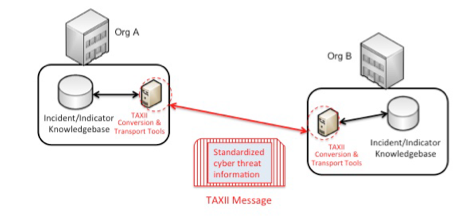
\includegraphics[scale=0.80]{./images/TAXIIArchitecture1.png}
    \caption{Arquitectura de TAXII \protect\cite{b1}}
    \label{fig.diagramabloques}
\end{figure}

TAXII utiliza protocolos y especificaciones existentes siempre que 
es posible, de esta forma se integra con mecanismos de intercambio de 
información para reducir los costos de implementación y permitir la adopción 
rápida por parte de organizaciones ya establecidas y que se encuentran 
intercambiando información.\\

Las motivaciones para tener una mejor solución que permita intercambiar 
información lleva a que en el diseño de TAXII se hayan planteado los siguientes 
objetivos:
 \begin{itemize}
   \item Permitir el intercambio seguro y rápido de información referente a 
   amenazas entre comunidades de defensores de seguridad.
   \item Lograr un estándar para permitir compartir indicadores entre organizaciones.
   \item Extender el intercambio de indicadores para permitir intercambios 
   seguros, robustos y de gran volumen que tengan una expresividad mayor a la 
   actual.
   \item Soportar un amplio número de casos de uso y prácticas comunes a las 
   comunidades.
   \item Tomar los estándares existentes que sean adecuados.
   \item Llegar a una adopción por parte de organizaciones internacionales de 
   estándares.
 \end{itemize}

Para automatizar el intercambio de información, es necesario especificar como 
ésta es compartida. Para lograr esto, TAXII define especificaciones técnicas y 
documentación de soporte. En particular, las especificaciones de TAXII definen 
un conjunto de capacidades necesarias para el transporte exitoso de mensajes. 
Los mensajes TAXII llevan datos de amenazas informáticas representados por medio de STIX. El conjunto completo de los mensajes incluyen mensajes con datos y 
de control.\\

\subsubsection{TAXII Toolkit}\ \\

Es provisto para soportar la adopción de TAXII y asistir en el desarrollo de 
capacidades compatibles. El \textit{toolkit} provee una colección de implementaciones de 
referencia, un conjunto de herramientas y una colección de librerías e 
interfaces.\\

TAXII está definido por múltiples especificaciones relacionadas. Esta sección 
describe las especificaciones definidas en TAXII.

\begin{itemize}
  \item \underline{Especificación de servicios}: Provee los requerimientos por los cuales se 
  definen los servicios e intercambios de TAXII. No provee detalles respecto al 
  formato de los datos o como los mensajes TAXII son transportados por la red. 
  Dichos detalles y requerimientos pueden ser encontrados en la especificación 
  de los protocolos de enlace y en la especificación de mensajes de enlace.
 \item \underline{Especificación de protocolos de enlace}: Define los requerimientos para 
 transportar mensajes TAXII por la red. Puede haber varias especificaciones 
 creadas para TAXII. Cada especificación define requerimientos para el 
 transporte de mensajes TAXII utilizando protocolos de red y se proveen 
 requerimientos respecto a como los servicios TAXII son soportados por los 
 protocolos de red.
 \item \underline{Especificación de mensajes de enlace}: Se definen requerimientos para 
 representar mensajes TAXII en un formato particular. Puede haber múltiples 
 especificaciones para dichos mensajes. Se provee información detallada sobre 
 como las especificaciones definidas en la especificación de servicios son 
 expresadas en los mensajes.
\end{itemize}

Para dar flexibilidad en el proceso evolutivo de TAXII, se han separado las 
especificaciones de servicios, de los protocolos de enlace y de los mensajes de 
enlace.
Debido a que las organizaciones generalmente tienen restricciones 
respecto a los protocolos que soportan, TAXII busca no ligarse a un único 
protocolo que excluya a una parte de la comunidad. Cuando se ve que la comunidad 
expresa interés en un nuevo protocolo o tipo de mensaje, TAXII puede dar soporte 
para ellos sin cambiar los componentes centrales.\\

Dos grupos que usen el mismo protocolo de red y formato de mensajes serán 
capaces de intercambios de información estructurada de forma automática. Las 
políticas de intercambio de los participantes pueden limitar estos intercambios 
si es necesario, pero el uso de servicios compatibles con TAXII asegura que se 
puede intercambiar cualquier información con los mecanismos definidos por TAXII. 
Los grupos que usen diferentes protocolos o formatos de mensajes no serán 
capaces de comunicarse directamente, pero como están utilizando mensajes y 
servicios en el núcleo de las comunicaciones de sus comunidades significa que es 
posible establecer caminos para que ocurra la interacción.

\subsubsection{Especificación de Servicios}\ \\

Esta especificación provee normativas respecto a los servicios, mensajes e 
intercambios de mensajes en TAXII. No provee detalles respecto a como los 
mensajes son transportados, dejando eso a la especificación de los protocolos de 
enlace. Se da información respecto a los datos presentes en los mensajes TAXII y 
no a como los mensajes son expresados.\\

Las unidades funcionales de TAXII representan conjuntos discretos de actividades 
requeridas para soportar TAXII. Una unidad funcional representa algún componente 
con un rol bien definido en TAXII.

\begin{itemize}
  \item \underline{TAXII Transfer Agent} (TTA): Es una unidad funcional conectada a la red 
  que envía o recibe mensajes TAXII. Una TTA interactúa con otras TTAs por medio 
  de la red y maneja los requerimientos de una o más de las especificaciones de 
  los protocolos de enlace. Una TTA provee un mensaje TAXII a un \textit{TAXII Message 
  Handler} permitiendo que éste último sea independiente del protocolo de red 
  utilizado. De la misma forma, el TTA puede ser independiente del contenido de 
  los mensajes TAXII, dejando el manejo de la información al \textit{TAXII Message 
  Handler}.
  \item \underline{TAXII Messsage Handler} (TMH): Es una unidad funcional que produce y 
  consume mensajes TAXII. EL TMH es responsable de parsear y construir mensajes 
  con el formato especificado en uno o más TAXII \textit{Message Binding Specifications}. 
  Un TMH interactúa con un TTA, el cual maneja los detalles necesarios para 
  transmitir mensajes por la red. El Backend TAXII interactúa con el TMH para 
  convertir su contenido en mensajes TAXII y llevar a cabo actividades basadas 
  en los mensajes TAXII que son recibidos por el TMH.
  \item \underline{Backend TAXII}: Cubre todas las unidades funcionales distintas al TTA y 
  al TMH. Las especificaciones de TAXII no proveen requerimientos sobre como son 
  implementadas las capacidades en un backend más allá de como debe interactuar 
  con el TMH. Las organizaciones o implementadores pueden decidir que 
  capacidades implementar según los servicios TAXII que deseen soportar o según 
  como quieran dar ese soporte.
  \item \underline{Arquitectura TAXII}: Cubre los aspectos de las unidades funcionales de la 
  infraestructura de productor o consumidor que provee o utiliza servicios 
  TAXII. Una arquitectura TAXII incluye una TTA, un TMH y un backend TAXII.
  \end{itemize}

Lo expresado anteriormente se puede ver en la figura \ref{fig.unidades_funcionales}.

\begin{figure}[ht!]
  \centering
    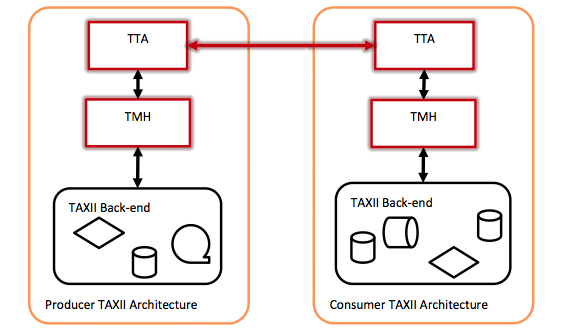
\includegraphics[width=150mm]{./images/TAXIIArchitecture.png}
    \caption{Unidades funcionales de TAXII \protect\cite{b1}}
    \label{fig.unidades_funcionales}
\end{figure}

\newpage
\subsubsection{Capacidades}\ \\

TAXII provee capacidades específicas para aquellos que desean compartir 
información de amenazas cibernéticas. Las capacidades TAXII son el nivel más 
alto en el cual se pueden expresar las acciones de TAXII. Hay tres capacidades 
que soporta la actual versión de TAXII, estas son: \textit{push messaging}, \textit{pull 
messaging} y \textit{discovery}.\\

En \textit{\textbf{push messaging}} la información puede ser enviada de un productor a un 
consumidor. Esto puede reflejar una relación pre-existente entre el productor y 
el consumidor en la que el consumidor ha pedido que se le envíen datos desde el 
productor. También puede usarse en caso de que el consumidor desee aceptar 
contribuciones de cualquier productor, y estos le envíen datos en cualquier 
momento.\\

\textit{\textbf{Pull messaging}} permite a un consumidor requerir información de un productor. 
Esto no solo le permite al consumidor el control sobre el momento en el que 
recibe los datos sino que también le permite hacerlo sin tener que aceptar 
conexiones entrantes. Así como en \textit{push messaging}, el productor y consumidor 
pueden tener acuerdos pre-existentes para que el consumidor tenga acceso a los 
datos del productor. De forma alternativa, un productor puede hacer su 
información pública de forma que cualquier consumidor pueda obtenerla. La 
versión actual de \textit{pull messaging} limita a los consumidores a hacer pedidos por 
medio de las organizaciones productoras de los datos en lugar de por los datos 
en si. Toda la información provista por un productor debe estar organizada en 
grupos llamados "TAXII Data Feeds". Cada elemento en un TAXII data feed es 
etiquetado utilizando \textit{timestamps}. El productor tiene total dominio sobre como el 
contenido se mapea en TAXII data feeds y en el significado de los \textit{timestamps}. La 
capacidad de \textit{pull messaging} está atada a entender el contenido del productor.\\

Para facilitar las comunicaciones automatizadas, TAXII soporta capacidades para 
descubrir los servicios específicos que ofrece un servidor o grupo de 
servidores, así como los protocolos o mensajes que este servidor ofrece. Esto no 
quita la necesidad de que personas estén involucradas para establecer acuerdos de 
cooperación lo cual esta por fuera del objetivo de TAXII. Sin embargo, permite 
el intercambio de información respecto a las capacidades que un productor 
soporta y cuales son los mecanismos que utiliza para hacerlo.

\subsubsection{Servicios TAXII}\ \\

Los servicios TAXII representan un conjunto de mecanismos necesarios para 
soportar capacidades TAXII. Una implementación TAXII pudiera implementar alguno, 
todos o incluso ninguno de los servicios definidos.
TAXII define los siguientes servicios:
\begin{itemize}
  \item \underline{Discovery Service}: Es utilizado para recibir y responder a 
  mensajes que requieren información sobre los servicios ofrecidos.
  \item \underline{Feed Managment Service}: Es utilizado para recibir o responder a mensajes 
  utilizados para el manejo de subscripciones a TAXII Data Feed.
  \item \underline{Inbox Service}: Es utilizado para recibir información de amenazas 
  cibernéticas por medio de intercambios iniciados por el productor en intervalos 
  dictados por este.
  \item \underline{Poll Service}: Es utilizado para recibir y responder a mensajes de pedido 
  a el TAXII Data Feed iniciados por el consumidor.
\end{itemize}

A continuación se describen los distintos servicios.

\paragraph{Discovery Service}\ \\

Es un mecanismo para comunicar información referente al uso de servicios TAXII y 
a su disponibilidad. Para un pedido al servicio, se retorna una lista de los 
servicios TAXII y como estos pueden ser invocados. Un solo servicio de 
descubrimiento puede reportar servicios TAXII en diferentes equipos finales o 
incluso en múltiples organizaciones, los propietarios del servicio pueden 
definir su alcance a gusto. Un servicio de descubrimiento puede utilizar 
varios factores para determinar cuales servicios revelar ante una petición, 
incluyendo, pero no limitado a la entidad del cliente TAXII.
El servicio de descubrimiento debe soportar "Discovery Message Exchange".

\paragraph{Feed Managment Service}\ \\

Es el mecanismo con el cual un consumidor pide información referente a TAXII 
Data Feeds, pidiendo subscripciones a estos, o modificando las existentes. Este 
servicio facilita el intercambio de mensajes para manejar las subscripciones. 
No se entrega contenido de los TAXII Data Feed, en su lugar se envía 
contenido del TAXII Data Feed al servicio de Inbox de un consumidor en intercambios 
iniciados por un productor o en respuesta directa a un pedido del consumidor al 
servicio de poll.
Dicho servicio debe implementar soporte para \textit{subscription managment exchange} y podría implementar soporte de \textit{feed information exchange}.

\paragraph{Inbox service}\ \\
Este servicio es el mecanismo con el cual un consumidor acepta los mensajes en 
un intercambio iniciado por el productor. Un consumidor puede implementarlo 
para recibir datos del TAXII Data Feed.
El servicio de inbox debe implementar soporte para \textit{Data Push Exchange}.

\paragraph{Poll service}\ \\
Es provisto por un productor para permitir pedidos al TAXII Data Feed iniciados 
por  el consumidor. Un consumidor contacta a este servicio explícitamente 
pidiendo el contenido del TAXII Data Feed. Los productores podrían ofrecer Data 
Feeds combinando envíos al Inbox service del consumidor o por medio de pedidos 
al servicio de poll del productor.
Una implementación de este servicio debe dar soporte a \textit{Data Poll Exchange}.

\subsubsection{Intercambio de mensajes TAXII}\ \\

Esta sección describe los mensajes intercambiados que son necesarios para soportar 
los servicios definidos antes. Estos intercambios solo consideran mensajes 
TAXII y son independientes a los protocolos sobre los cuales viajan los mensajes.
 En particular, esos protocolos podrían requerir intercambios de red 
adicionales antes de transmitir mensajes TAXII o romper un mensaje TAXII en 
múltiples mensajes del protocolo subyacente que son transmitidos 
independientemente.

\paragraph{Data Push Exchange}\ \\
En este intercambio, un mensaje STIX es transmitido desde un cliente a un 
servidor inbox que está esperando. El mensaje STIX puede ser solicitado o no 
solicitado. El servidor inbox puede ser capaz de filtrar mensajes según la 
autenticidad del emisor.

\paragraph{Discovery Exchange}\ \\

Un cliente TAXII pide información sobre el servicio TAXII ofrecido por un 
productor. El discovery server del productor responde con una lista de 
servicios. 

El cliente TAXII envía un pedido de descubrimiento al servidor. El Backend TAXII podría utilizar esta 
información junto a su propia política de control de acceso  para crear una 
lista de servicios a ser retornada. Estos son empaquetados en una 
respuesta de discovery la cual es enviada al cliente TAXII. El 
cliente TAXII recibe esa respuesta y la pasa la información del servicio a su 
propio BackEnd para ser procesado.

\paragraph{Feed Information Exchange}\ \\

En este intercambio un cliente TAXII pide información sobre fuentes de datos disponibles en 
un Feed Server. El servidor responde con una lista de fuentes de datos 
de las que dispone. Dicha respuesta es realizada por el backend y en ella se pueden considerar decisiones de control de acceso.\\

\paragraph{Subscription Managment Exchange}\ \\

En este un cliente intenta establecer, borrar, pausar, resumir o modificar una 
subscripción a un TAXII Data Feed conocido enviando un mensaje subscription 
managment request al servidor. El servidor pasa la request al Backend TAXII el 
cual determina la respuesta, la cual es luego enviada al cliente.
El backend TAXII puede usar dicha información junto con sus 
políticas de control de acceso y las funcionalidades que posea para determinar 
si la acción está permitida o no.

\paragraph{Feed Poll Exchange}

Es utilizado por un consumidor para pedir contenido de un productor de datos. El TAXII Data Feed content es enviado al consumidor en el mismo intercambio.
El cliente consumidor inicia el backend TAXII y evalua el pedido de información para determinar la respuesta. La respuesta retorna mensajes STIX con el contenido que pidió el cliente.
 
%\subsubsection{Modelos}
%\label{anexo.modelos}
%\subsubsection{Comunidades}
Actualmente el número de organizaciones que buscan compartir información de
amenazas es creciente. Esto lleva a que el número y tipo de comunidades que busca
hacerlo también se incremente. En la actualidad se identifican tres tipos de comunidades:
\begin{itemize}
  \item Pares
  \item Comerciales
  \item Gubernamentales
\end{itemize}

Para que se pueda compartir información entre dichas organizaciones es necesario
cierto nivel de confianza dado que compartir información sensible podría exponer 
a las organizaciones a daños en su reputación, demandas o advertir a un 
atacante de la investigación que se lleva a cabo haciendo que el trabajo 
realizado haya sido inútil. Se deben definir medidas para la protección de los 
datos como restricciones en su manejo, sanitización y el establecimiento de 
confianza entre las dos organizaciones. Lo mencionado anteriormente es 
particularmente importante cuando las organizaciones forman parte de varias 
comunidades que intercambian información, se encuentran casos en los que datos 
compartidos con una organización no deberían ser compartidos con otra.\\

Las comunidades entre \textbf{pares} son las más comunes, estas organizaciones o 
individuos tienen el propósito común de mejorar las defensas colectivas contra 
adversarios que tienen en común. La información compartida por dichas 
organizaciones es más especifica que la provista por organizaciones comerciales.\\

Las comunidades \textbf{comerciales} son anónimas y los miembros poseen algún tipo de 
acuerdo común, por ejemplo el pago de cuotas para pertenecer a la comunidad. 
La organización comercial maneja la información de forma centralizada y la 
distribuye entre los miembros de la organización. El acceso a la información por 
parte de los socios es rápido teniendo la posibilidad de que dicha información 
sea más amplia que la compartida por pares y que además no siempre sea aplicable a las 
necesidades de la organización.\\

Las comunidades \textbf{gubernamentales} son establecidas y manejadas por el gobierno, 
son voluntarias u obligatorias e incluyen participantes tanto del gobierno como 
de la industria privada. En ellas el gobierno controla la información y la 
distribución de esta. Así como en las comunidades comerciales, la información y 
los participantes son altamente confidenciales.\\

\subsubsection{Modelos}

Se pueden identificar tres modelos para el intercambio de información entre 
organizaciones:
\begin{itemize}
  \item Hub and Spoke
  \item Peer to peer
  \item Source/subscriber
\end{itemize}

En el método \textbf{hub and spoke}, la entidad hub controla la recepción y diseminación 
de los datos, además se encarga de mantener anónimos y proveer un análisis 
adicional de los datos recolectados para luego diseminarlos entre los 
participantes. Este modelo es comúnmente visto en comunidades de gobierno o comerciales.\\

En el modelo \textbf{peer to peer}, los participantes intercambian y reciben información 
directamente de los otros participantes. La información es compartida entre 
todos los miembros de la comunidad por igual y la fuente está claramente 
identificada.\\

\textbf{Source/subscriber} es utilizado por las 
comunidades comerciales que proveen de información. El proveedor de información 
envía regularmente información a todos los subscriptores y estos podrían 
eventualmente enviarle información a la fuente. Generalmente, la información se 
codifica de una manera propietaria y puede faltar información esencial sobre 
algunos intentos de irrupción. Presenta la ventaja de que se tiene acceso rápido 
a un conjunto de datos amplio y es útil para organizaciones con recursos 
limitados.\\

\subsubsection{Implementación de Modelos en TAXII}

A continuación se muestra como los servicios TAXII pueden ser utilizados para la 
implementación de los modelos para el intercambio de información.

\paragraph{Source/Suscriber}\ \\

En este modelo una entidad es la fuente de información y algunos subscriptores 
tienen acuerdos con dicha entidad para recibir información periódicamente. Se 
busca que los subscriptores no se conozcan entre si, para ello la entidad fuente 
realiza acuerdos con cada uno de ellos. En este modelo, la fuente es 
un productor TAXII mientras que los subscriptores son consumidores.\\

TAXII soporta este tipo de modelo para el intercambio con el uso de los servicios de 
Discovery, Feed Management, Inbox y Poll. Una organización que desee 
subscribirse al TAXII Data Feed de la fuente necesita conocer los servicios 
TAXII que la fuente ofrece y como contactar con ellos. Si bien esto podría ser 
realizado por una mecanismo fuera de banda (e.g. publicando la información en otro medio)
también podría ser logrado contactando al Discovery Service de la fuente. Desde 
este punto, el subscriptor podría contactar al servicio de Feed Managment 
identificado para aprender que fuentes ofrece el productor y que restricciones 
podría tener su acceso.\\

Si el contenido del TAXII Data Feed es restringido solo a algunas entidades 
autorizadas y el productor ha determinado que el subscriptor tiene permitido 
recibir el contenido, la fuente y el subscriptor necesitan acordar en como el 
subscriptor se autenticara. Dependiendo en el protocolo que soporta la fuente, 
esto se puede realizar por medio de una contraseña, un certificado u otro método. 
Si el contenido de un TAXII Data Feed es abierto y no requiere 
autenticación, éste paso es innecesario cuando se establecen las subscripciones 
al TAXII Data Feed.\\

Luego de la autenticación,el subscriptor puede contactar al Feed Managment Service del 
productor y pedir subscripciones a sus fuentes. La entidad fuente puede 
comparar dichos pedidos con su propio entendimiento de lo que el subscriptor 
puede recibir y permitir o denegar dichos pedidos según corresponda. La fuente 
puede enviar contenido al subscriptor al Inbox Service de éste en el intervalo 
apropiado. Alternativamente, el subscriptor podría contactar al Poll service de 
la fuente para descargar el contenido deseado.\\

\begin{figure}[ht!]
 
  \centering
  	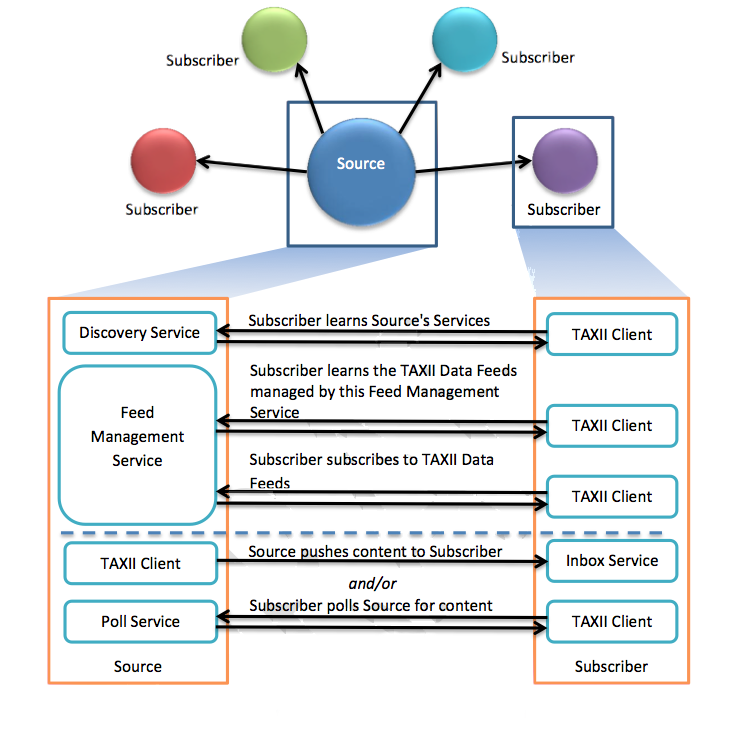
\includegraphics[width=150mm]{./images/SourceSuscriberModel.png}
    \caption{Flujo de información en modelo Source/Subscriber \protect\cite{b1}}
    \label{fig.sourcesuscribermodel}
\end{figure}

La figura \ref{fig.sourcesuscribermodel} muestra como el modelo Source/Subscriber puede ser soportado por los 
servicios TAXII. También se ven los mensajes TAXII intercambiados entre la
fuente y el subscriptor. Con los intercambios que están por encima de la línea 
punteada se establece la subscripción. Los intercambios pueden ser realizados 
repetidamente sin la necesidad de realizar el proceso de subscripción 
nuevamente.

\newpage

\paragraph{Peer-to-peer}\ \\ 

En un modelo Peer-to-peer, los pares de organizaciones entran en un acuerdo 
mutuo para compartir información entre si. En este modelo, cada Peer puede 
operar como productor y consumidor. Los socios en este intercambio podrían 
establecer fuentes utilizando un procedimiento similar al establecido en el 
modelo Source/Subscriber. Alternativamente, podrían acordar subir o descargar 
contenido sin ninguna subscripción formal. No tener una subscripción formal 
permite a un Peer albergar un Inbox Service sin necesidad de un Feed 
Managment Service.\\

El modelo Peer-to-Peer tiene dos variantes: acuerdos para el intercambio entre 
comunidades y acuerdos para el intercambio ad-hoc. En el primero la comunidad 
constituye acuerdos entre pares en los que todos los miembros acuerdan una única 
política la cual será respetada por todos. A diferencia de los otros dos 
modelos que tienen un punto central desde el cual la información es diseminada, 
todo el intercambio ocurre puntualmente entre dos pares. Si los pares A y B 
desean recibir información del peer C directamente, ambos necesitaran 
establecer un acuerdo apropiado con el peer C para que éste les envíe la 
información que desean.\\

Alternativamente, el intercambio entre pares puede ser realizado de forma 
individual con intercambios ad-hoc. Esto podría ocurrir si dos compañías hacen 
acuerdos individuales para compartir entre ellas. En este caso, los acuerdos 
sobre que compartir son específicos para las partes. Una sola entidad podría 
participar en ambas variantes, perteneciendo a una o mas comunidades en las 
cuales los miembros comparten entre si siguiendo un acuerdo común entre los 
miembros y a su vez negocian acuerdos individuales con otras entidades. Alguna 
información recibida por medio de un acuerdo no siempre debería ser compartida 
con otros pares que no son parte del acuerdo. De esta forma un participante 
debería hacer un seguimiento de quien fue el proveedor de la información 
recibida, como se realiza ese seguimiento está por fuera de la especificación de 
TAXII.\\

\begin{figure}[ht!]
  \centering
  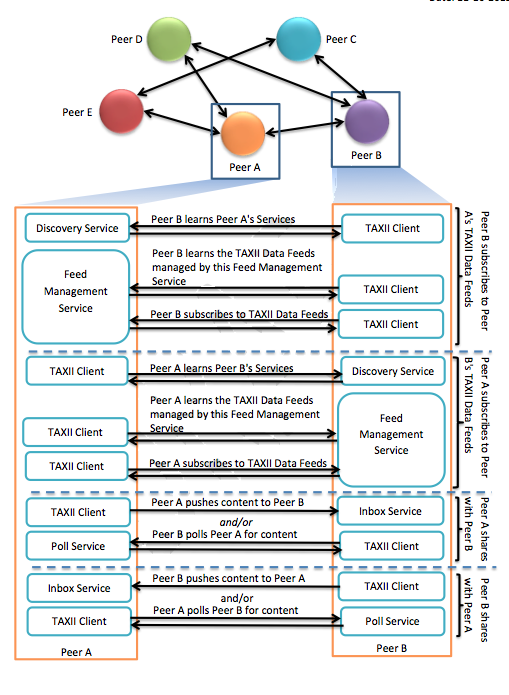
\includegraphics[scale=0.55]{./images/PeerToPeerModel.png}
    \caption{Flujo de información en modelo Peer to Peer \protect\cite{b1}}
  \label{fig.peertopeermodel}
\end{figure}

La figura \ref{fig.peertopeermodel} muestra como el modelo Peer to peer puede ser realizado por 
medio de los servicios TAXII. En este diagrama se ve que dos pares se contactan 
para pedir subscripciones para obtener información. Se asume que ambos pares 
tienen un Feed Managment Service que es utilizado para manejar todos los 
pedidos de subscripción.
\newpage

\paragraph{Hub and Spoke}\ \\

En un modelo Hub and Spoke, la entidad Hub es un consumidor de 
información que le proveen las entidades Spoke, pero a su vez se comporta como
un productor que brinda información a entidades 
Spoke. Una entidad Spoke podría ser un productor, dando información al Hub, un 
consumidor que reciba actualizaciones del Hub o ambas. El Hub puede utilizar un 
Inbox Service para recibir información de cualquiera que desee enviar 
información de forma voluntaria y/o podría requerir información de ciertas 
fuentes para guardar la información en una única ubicación. Desde este punto, el 
Hub puede funcionar como una entidad Source del modelo Source/Subscriber 
mientras que los Spoke serían Subscribers de dicho modelo. El Hub puede adoptar 
cualquier política respecto de la información que recibe, desde pasar toda la 
información automáticamente a solo pasar información de socios reconocidos, o 
realizar ediciones y análisis antes de reenviar la información.

\begin{figure}[ht!]
  \centering
    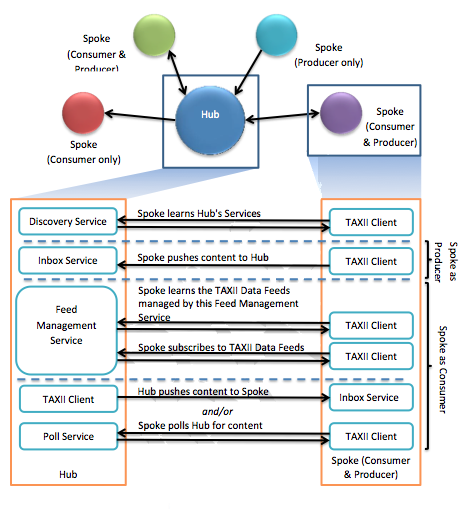
\includegraphics[scale=0.75]{./images/HubAndSpokeModel.png}
    \caption{Flujo de información en modelo Hub and Spoke \protect\cite{b1}}
    \label{fig.hubandspokemodel}
\end{figure}

La figura \ref{fig.hubandspokemodel} muestra como se puede implementar el modelo Hub and Spoke 
utilizando los servicios provistos por TAXII. En este modelo algunas entidades 
Spoke podrían ser consumidores, otras productores y en algunos casos ambas. El 
diagrama muestra los intercambios que podrían ser utilizados por el Spoke que 
actúa como productor y consumidor. Si este desea actuar de una sola forma solo 
los intercambios necesarios serían relevantes. Independientemente del rol que 
tome el Spoke, es necesario que éste conozca los servicios relevantes en el Hub. 
Esto se realiza utilizando el Discovery Service provisto por el Hub, de todas 
formas esto podría realizarse con mecanismos fuera de banda.



 

\chapter{Implementación}
\subsection{Servicios TAXII Implementados}
	
	\begin{center}
		\begin{tabular}{|l|}
			\hline
			def inbox\_service(request, inbox\_name): \\
			"""Handles TAXII Inbox Service requests.""" \\ \\
			
			def poll\_service(request):\ \\
			"""Handles TAXII Poll Service requests.""" \\ \\
			
			def feed\_managment\_service(request): \\
			"""Handles TAXII Feed Managment Service requests.""" \\ \\
			
			def subscription\_service(request):\ \\
			"""Handles TAXII Subscription Service requests.""" \\
			\hline
		\end{tabular}
	\end{center}\ \\

\chapter{API REST implementada}

	\begin{center}
		\begin{tabular}{|l|}
			\hline
			class UserViewSet(viewsets.ModelViewSet):\\
			\#Gets, lists, creates or updates users.\\ \\
			
			class ProtocolBindingIdViewSet(viewsets.ModelViewSet):\\
			\#Gets, lists, creates or updates ProtocolBindingIds\\ \\
			
			class ContentBindingIdViewSet(viewsets.ModelViewSet):\\
			\#Gets, lists, creates or updates ContentBindingIds\\ \\
			
			class MessageBindingIdViewSet(viewsets.ModelViewSet):\\
			\#Gets, lists, creates or updates MessageBindingIds\\ \\
			
			class DataFeedPushMethodViewSet(viewsets.ModelViewSet):\\
			\#Gets, lists, creates or updates DataFeedPushMethods\\ \\
			
			class DataFeedPollInformationViewSet(viewsets.ModelViewSet):\\
			\#Gets, lists, creates or updates DataFeedPollInformations\\ \\
			
			class RemoteDataFeedPollInformationViewSet(viewsets.ModelViewSet):\\
			\#Gets, lists, creates or updates RemoteDataFeedPollInformations\\ \\
			
			class DataFeedSubscriptionMethodViewSet(viewsets.ModelViewSet):\\
			\#Gets, lists, creates or updates DataFeedSubscriptionMethods\\ \\
			
			class ContentBlockViewSet(viewsets.ModelViewSet):\\
			\#Gets, lists, creates or updates ContentBlocks\\ \\
			
			class DataFeedViewSet(viewsets.ModelViewSet):\\
			\#Gets, lists, creates or updates DataFeeds\\ \\
			
			class RemoteDataFeedViewSet(viewsets.ModelViewSet):\\
			\#Gets, lists, creates or updates RemoteDataFeeds\\ \\
			
			class DataFeedSubscriptionViewSet(viewsets.ModelViewSet):\\
			\#Gets, lists, creates or updates SubscriptionFeeds\\
			
			\hline
		\end{tabular}
	\end{center}
	\newpage
	\begin{center}
		\begin{longtable}{|l|}
			\hline
			
			class InboxViewSet(viewsets.ModelViewSet):\\
			\#Gets, lists, creates or updates Inboxes\\ \\
			
			class RemoteInboxViewSet(viewsets.ModelViewSet):\\
			\#Gets, lists, creates or updates RemoteInboxes\\ \\
			
			class ContentBlockRTIRViewSet(viewsets.ModelViewSet):\\
			\#Gets, lists, creates or updates ContentBlockRTIRs\\ \\
			
			class TAXIIServicesViewSet(viewsets.ModelViewSet):\\
			\#Gets, lists, creates or updates TAXIIServices\\ \\
			
			class FeedManagmentServicesViewSet(viewsets.ModelViewSet):\\
			\#Gets, lists, creates or updates FeedManagementServices\\ \\
			
			
			def get\_remote\_data\_feeds(request):\\
			\#Given the id of a TAXII Service we make a FeedInformation request to\\ that service address.\\
			\#The response is a list of the feed names of the TAXII client and\\ a list of all protocol bindings,\\ content binding and message binding.\\ \\
			
			def register\_remote\_data\_feeds(request):\\
			\#Given the id of a TAXII service we get the data feeds of the TAXII Client and\\ copy them to the current system.\\ \\
			
			def create\_information(request):\\
			\#When in GET method return all the Content Blocks.\\
			\#When in POST method, given a content binding id, a title, description and content\\ we create a Content Block.\\ \\
			
			def send\_information\_to\_inbox(request):\\
			\#Given the id of a DataFeed Subscription we get the Data Feeds and send it to\\ send it to the inbox service of the organization of the subscription service.\\ \\
			
			def poll\_information(request):\\
			\#Given the id of a remote data feed,\\ we get the poll service instances and for each make a poll request.\\ \\
			
			def get\_data\_feed\_subscriptions(request):\\
			\#We get all the date feed subsctiptions and\\ return the id, adress and data feed name of each.\\ \\
			
			def subscription\_to\_data\_feed(request):\\
			\#Given the id of a TAXII Service and the id of a Data Feed and\\ the service id we make a Manage Feed Subscription request for that Data Feed.\\		
			
			\hline
		\end{longtable}
	\end{center}
	\newpage

\section{Entidades desarrolladas utilizadas}
	
	\begin{center}
		\begin{longtable}{|l|}
			\hline

	class ProtocolBindingId():\\
	    """\\
	    Represents a protocol binding id, used to establish the exchange protocol\\
	    supported by a TAXII implementation.\\
	    Ex:\\
	    HTTP protocol binding id : "urn:taxii.mitre.org:protocol:http:1.0"\\
	    HTTPS protocol binding id : "urn:taxii.mitre.org:protocol:https:1.0"\\
	    """\\
	    title = CharField(blank=True)\\
	    description = TextField(blank=True)\\
	    bindingid = CharField(maxlength=MAXIDLEN)\\
	    datecreated = DateTimeField(autonowadd=True)\\
	    dateupdated = DateTimeField(autonow=True)\\
	\\
	class ContentBindingId():\\
	    """\\
	    Represents a content binding id, used to establish the supported content\\
	    types for a given TAXII exchange (e.g., Poll, Inbox, etc.).\\
	    Ex:\\
	    STIX v1.0 content binding id : "urn:stix.mitre.org:xml:1.0"\\
	    """\\
	    title = CharField(blank=True)\\
	    description = TextField(blank=True)\\
	    bindingid = CharField(maxlength=MAXIDLEN)\\
	    datecreated = DateTimeField(autonowadd=True)\\
	    dateupdated = DateTimeField(autonow=True)\\
	\\
	class MessageBindingId():\\
	    """\\
	    Represents a message binding id, used to establish the supported syntax\\
	    for a given TAXII exchange, "e.g., XML".\\
	    Ex:\\
	    XML message binding id : "urn:taxii.mitre.org:message:xml:1.0"\\
	    """\\
	    title = CharField(blank=True)\\
	    description = TextField(blank=True)\\
	    bindingid = CharField(maxlength=MAXIDLEN)\\
	    datecreated = DateTimeField(autonowadd=True)\\
	    dateupdated = DateTimeField(autonow=True)\\
	\\
	class DataFeedPushMethod():\\
	    """\\
	    Used to establish the protocols that can be used to push content via\\
	    a subscription. This appears in a Feed Information Response message,\\
	    as defined by the TAXII Services Specification.\\
	    """\\
	    title = CharField(blank=True)\\
	    description = TextField(blank=True)\\
	    protocolbinding = ForeignKey(ProtocolBindingId)\\
	    messagebinding = ForeignKey(MessageBindingId)\\
	    datecreated = DateTimeField(autonowadd=True)\\
	    dateupdated = DateTimeField(autonow=True)\\
	\\
	class DataFeedPollInformation():\\
	    """\\
	    Used to establish the supported protocols and address of a Data Feed.\\
	    This appears in a Feed Information Response message, as defined by the\\
	    TAXII Services Specification.\\
	    """\\
	    title = CharField(blank=True)\\
	    description = TextField(blank=True)\\
	    address = URLField()\\
	    protocolbinding = ForeignKey(ProtocolBindingId)\\
	    messagebindings = ManyToManyField(MessageBindingId)\\
	    datecreated = DateTimeField(autonowadd=True)\\
	    dateupdated = DateTimeField(autonow=True)\\
	\\
	class DataFeedSubscriptionMethod():\\
	    """\\
	    Used to identify the protocol and address of the TAXII daemon hosting\\
	    the Feed Management Service that can process subscriptions for a TAXII\\
	    Data Feed. This appears in a Feed Information Response message, as defined\\
	    by the TAXII Services Specification.\\
	    """\\
	    title = CharField(blank=True)\\
	    description = TextField(blank=True)\\
	    address = URLField()\\
	    protocolbinding = ForeignKey(ProtocolBindingId)\\
	    messagebindings = ManyToManyField(MessageBindingId)\\
	    datecreated = DateTimeField(autonowadd=True)\\
	    dateupdated = DateTimeField(autonow=True)\\
	\\
	class ContentBlock():\\
	    """Represents the content block of a TAXII Poll Response or Inbox message."""\\
	    title = CharField(blank=True) \# not required by TAXII\\
	    description = TextField(blank=True) \# not required by TAXII\\
	    timestamplabel = DateTimeField(default=lambda:datetime.datetime.now(tzutc()))\\
	    submittedby = ForeignKey(User, blank=True, null=True)\\
	    messageid = CharField(blank=True)\\
	    contentbinding = ForeignKey(ContentBindingId)\\
	    content = TextField()\\
	    padding = TextField(blank=True)\\
	    datecreated = DateTimeField(autonowadd=True)\\
	    dateupdated = DateTimeField(autonow=True)\\
	\\
	class DataFeed():\\
	    """Represents a TAXII Data Feed"""\\
	    name = CharField()\\
	    description = TextField(blank=True)\\
	    users = ManyToManyField(User, blank=True, null=True)\\
	    supportedcontentbindings = ManyToManyField(ContentBindingId)\\
	    pushmethods = ManyToManyField(DataFeedPushMethod)\\
	    pollserviceinstances = ManyToManyField(DataFeedPollInformation)\\
	    subscriptionmethods = ManyToManyField(DataFeedSubscriptionMethod, \\
	    					blank=True, null=True)\\
	    contentblocks = ManyToManyField(ContentBlock, blank=True, null=True)\\
	    datecreated = DateTimeField(autonowadd=True)\\
	    dateupdated = DateTimeField(autonow=True)\\
	\\
	class DataFeedSubscription():\\
	    """Represents a Data Feed Subscription. This is not used by TAXII at the moment."""\\
	    subscriptionid = CharField(unique=True) \# uri formatted subscription id\\
	    user = ForeignKey(User)\\
	    datafeed = ForeignKey(DataFeed)\\
	    datafeedmethod = ForeignKey(DataFeedSubscriptionMethod)\\
	    active = BooleanField(default=True)\\
	    expires = DateTimeField()\\
	    datecreated = DateTimeField(autonowadd=True)\\
	    dateupdated = DateTimeField(autonow=True)\\
	\\
	class Inbox():\\
	    """\\
	    Characterizes a TAXII Inbox. Inboxes are the mechanism by which TAXII consumers\\
	    receive data from TAXII publishers. This Inbox implementation allows an Inbox\\
	    to be "bound" to zero or more Data Feeds, meaning that data received by an Inbox\\
	    can populate Data Feeds if a user configures it as such.\\
	    """\\
	    name = CharField(unique=True)\\
	    description = TextField(blank=True)\\
	    supportedcontentbindings = ManyToManyField(ContentBindingId)\\
	    supportedmessagebindings = ManyToManyField(MessageBindingId)\\
	    contentblocks = ManyToManyField(ContentBlock, blank=True, null=True)\\
	    supportedprotocolbinding = ForeignKey(ProtocolBindingId)\\
	    datafeeds = ManyToManyField(DataFeed, blank=True, null=True)\\
	    users = ManyToManyField(User, blank=True, null=True)\\
	    datecreated = DateTimeField(autonowadd=True)\\
	    dateupdated = DateTimeField(autonow=True)\\
	\\
	class ContentBlockRTIR():\\
	    """Represents the nexus between the RTIR ticket and the content block."""\\
	    rtirid = IntegerField(unique=True)\\
	    contentblock = ForeignKey(ContentBlock)\\
	\\
	class RemoteDataFeedPollInformation():\\
	    """Represents DataFeed Poll Information of remote TAXII clients """\\
	    title = CharField(blank=True)\\
	    description = TextField(blank=True)\\
	    address = URLField()\\
	    protocolbinding = ForeignKey(ProtocolBindingId)\\
	    messagebindings = ManyToManyField(MessageBindingId)\\
	    datecreated = DateTimeField(autonowadd=True)\\
	    dateupdated = DateTimeField(autonow=True)\\
	\\
	class RemoteDataFeed():\\
	    """Represents DataFeeds of remote TAXII clients """\\
	    name = CharField(maxlength=MAXTITLELEN)\\
	    description = TextField(blank=True)\\
	    supportedcontentbindings = ManyToManyField(ContentBindingId)\\
	    pushmethods = ManyToManyField(DataFeedPushMethod)\\
	    pollserviceinstances = ManyToManyField(RemoteDataFeedPollInformation, null=True)\\
	    subscriptionmethods = ManyToManyField(DataFeedSubscriptionMethod, \\
	    blank=True, null=True)\\
	    contentblocks = ManyToManyField(ContentBlock, blank=True, null=True)\\
	    datecreated = DateTimeField(autonowadd=True)\\
	    dateupdated = DateTimeField(autonow=True)\\
	\\
	class RemoteInbox():\\
	    """Represents Inboxes of remote TAXII clients """\\
	    name = CharField(unique=True) \\ \# this will become part of the URL where it can be accessed at\\
	    description = TextField(blank=True)\\
	    supportedcontentbindings = ManyToManyField(ContentBindingId)\\
	    supportedmessagebindings = ManyToManyField(MessageBindingId)\\
	    supportedprotocolbinding = ForeignKey(ProtocolBindingId)\\
	    datafeed = ForeignKey(DataFeed, blank=True)\\
	    address = URLField()\\
	    datecreated = DateTimeField(autonowadd=True)\\
	    dateupdated = DateTimeField(autonow=True)\\
	\\
	class TAXIIServices():\\
	    """Represents all TAXII Services available """\\
	    name = CharField(unique=True)\\
	    description = TextField(blank=True)\\
	    inbox = URLField()\\
	    poll = URLField()\\
	    feedmanagment = URLField()\\
	    subscription = URLField()\\
\\

			
			\hline
		\end{longtable}
	\end{center}
	
\section{Cyber Obsevables utilizados en el caso de estudio}

	\lstset{
		 breaklines=true
	}
    \lstinputlisting{cybox/CybOX\_Artifact\_Instance.xml}
    \lstinputlisting{cybox/CybOX\_Artifact\_Pattern.xml}
    \lstinputlisting{cybox/CybOX\_CreateFile\_Action.xml}
    \lstinputlisting{cybox/CybOX\_Domain\_Instance.xml}
    \lstinputlisting{cybox/CybOX\_Domain\_Pattern.xml}
    \lstinputlisting{cybox/CybOX\_IPv4Address\_Instance.xml}
    \lstinputlisting{cybox/CybOX\_IPv4Address\_Pattern.xml}
    \lstinputlisting{cybox/CybOX\_IPv6Address\_Instance.xml}
    \lstinputlisting{cybox/CybOX\_IPv6Address\_Pattern.xml}
    \lstinputlisting{cybox/CybOX\_Iran-Oil\_Dynamic.xml}
    \lstinputlisting{cybox/CybOX\_Network\_Connection\_HTTP\_Instance.xml}
    \lstinputlisting{cybox/CybOX\_Network\_Connection\_HTTP\_Pattern.xml}
    \lstinputlisting{cybox/CybOX\_Network\_Connection\_Instance.xml}
    \lstinputlisting{cybox/CybOX\_Network\_Connection\_Pattern.xml}
    \lstinputlisting{cybox/CybOX\_PDF\_File\_Instance.xml}
    \lstinputlisting{cybox/CybOX\_PDF\_File\_Pattern.xml}
    \lstinputlisting{cybox/CybOX\_Simple\_Email\_Instance.xml}
    \lstinputlisting{cybox/CybOX\_Simple\_Email\_Pattern.xml}
    \lstinputlisting{cybox/CybOX\_Simple\_File\_Instance.xml}
    \lstinputlisting{cybox/CybOX\_Simple\_File\_Pattern.xml}
    \lstinputlisting{cybox/CybOX\_Simple\_File\_Pattern\_Regex.xml}
    \lstinputlisting{cybox/CybOX\_URL\_Instance.xml}
    \lstinputlisting{cybox/CybOX\_URL\_Pattern.xml}
    \lstinputlisting{cybox/CybOX\_X509\_Certificate\_Instance.xml}
    \lstinputlisting{cybox/CybOX\_X509\_Certificate\_Pattern.xml}

\end{document}
